% Chapter Template

\chapter{Datos} % Main chapter title

\label{Cap_Data} % Change X to a consecutive number; for referencing this chapter elsewhere, use \ref{ChapterX}


%Justificación de la importancia de graficar los datos antes de realizar análisis estadísticos.
Antes de realizar los análisis estadísticos necesarios para determinar si los datos obtenidos arrojan evidencia sobre la existencia del llamado Efecto Espejo en las tarea de detección perceptual propuestas, se construyeron una serie de gráficos para explorar exhaustivamente la ejecución de los participantes. Graficar los datos disponibles antes de proceder a su análisis constituye una práctica altamente recomendada, no sólo porque permite evaluar la pertinencia de los experimentos propuestos a la luz de las respuestas de los participantes, sino porque constituye un primer filtro para revisar los datos registrados, descartando la posibilidad de que los participantes estuvieren respondiendo de acuerdo a patrones independientes de las tareas presentadas y procurando que toda interpretación o conclusión que pueda resultar de su análisis sea coherente y confiable.\\

%Presentación de los controles graficados: Atención, El efecto del paso del tiempo y las variables externas en los estímulos. 
Los gráficas que se presentan en este capítulo exploran las posibles relaciones que pudieran guardar las respuestas de los participantes con cualquier variable ajena a las demandas de la tarea, como podrían ser las respuestas inmediatamente anteriores, el paso del tiempo (i.e. aprendizaje) y las propiedades de los estímulos diseñados. Evaluar dichas correlaciones se considera un paso importante para controlar que los datos obtenidos provengan de participantes que estuvieran atendiendo la tarea, cuyo desempeño no mostrara cambios a lo largo del tiempo y que no se vieran influenciados por cualquier otra característica de los estímulos cosntruidos que no sea el número de círculos externos en las figuras de Ebbinghaus, (i.e. la única variable con que intencionalmente se manipulan los niveles de discriminabilidad).\\


\section{Control 1: ¿Los participantes estaban poniendo atención a la tarea para emitir una respuesta?}

%Evaluando la atención: Que
Los experimentos realizados estuvieron compuestos de 640 ensayos, a lo largo de los cuales los participantes tuvieron que decidir si los estímulos presentados cumplían con la condición que se les solicitó detectar y además, valorar su certidumbre sobre esta primer respuesta y asignarle un puntaje. Con un procedimiento tan demandante y extenso, es natural cuestionar la atención con que los participantes pudieran estar respondiendo a lo largo del experimento. Por lo tanto, nuestro primer control consistió en revisar la emisión de respuestas ensayo a ensayo para verificar que no se presentaran trenes de respuesta independientes del contenido de la tarea y supervisar que todas las opciones de respuesta fueran utilizadas en un proporciones razonables (sobretodo en el caso de la Escala de Confianza).\\

\begin{itemize}
\item Emisión de respuestas 'Sí/No' a lo largo del experimento.

Primero graficamos las respuestas emitidas ensayo a ensayo durante la tarea de detección binaria ('Sí, los círculos son iguales', 'No, los círculos son diferentes'). El objetivo principal de estas gráficas fue el de detectar trenes de respuesta exhacerbados que, dada la aleatoriedad con que el programa presentó los estímulos diseñados, pudieran delatar un sesgo del participante a oprimir una tecla en particular independientemente del estímulo a evaluar. La Figura~\ref{fig:Resp_E1_P1} presenta un ejemplo de este tipo de gráficas que ilustra la importancia de revisar los datos antes de incluirlos en el análisis estadístico y extraer conclusiones. Se trata del Participante 1 del Experimento 1, quien pasó los primeros 80 ensayos del experimento respondiendo repetidamente a la tecla 'No', este tren de respuesta es lo suficientemente largo como para cuestionar la atención con que el Participante estuvo respondiendo a la tarea.\\ 

\begin{figure}[th]
\centering
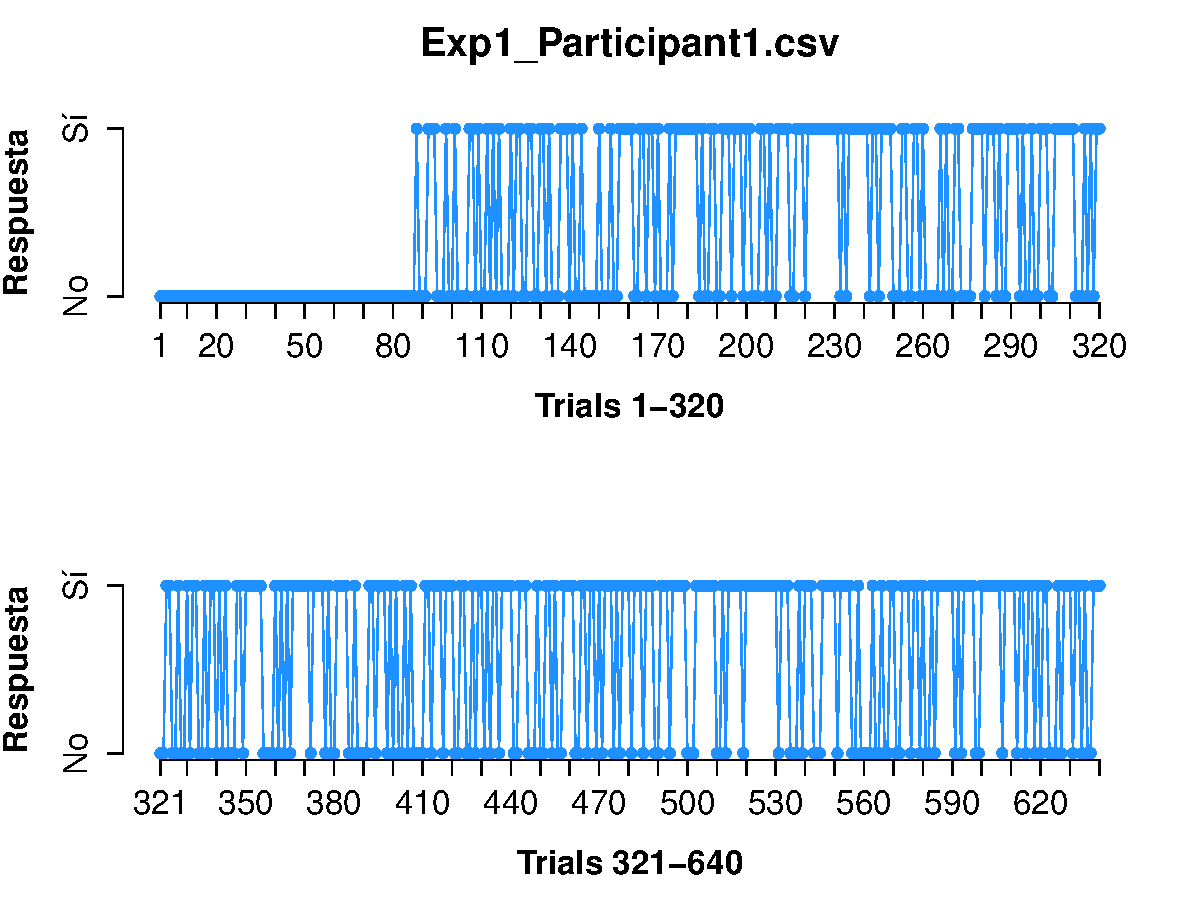
\includegraphics[width=0.50\textwidth]{Figures/Response_Exp1_P1} 
%\decoRule
\caption[Respuesta emitida por ensayo; ejemplo de participante sesgado]{Se muestran ls respuestas ('Sí/No') emitidas en cada uno de los ensayos por el Participante 1 del Experimento 1. La gráfica superior muestra las respuestas dadas durante los primeros 320 ensayos, y la gráfica inferior muestra el resto. Este gráfico delata un tren de respuesta que se extiende a lo largo de los primeros 80 ensayos, donde el participante sólo utilizó una de las opciones de respuesta.}
\label{fig:Resp_E1_P1}
\end{figure}

Las Figuras~\ref{fig:Response_P1} y \ref{fig:Response_E2} muestran las gráficas correspondientes al resto de los participantes en los Experimentos 1 y 2, respectivamente.\\

\item Correlación entre las respuestas 'Sí/No' emitidas y el tipo de estímulo presentado en cada ensayo.

Como una extensión de las gráficas ya mencionadas, se realizaron gráficos que además de señalar la respuesta dada por los participantes a la tarea de detección binaria ensayo a ensayo, permitiera identificar el tipo de estímulo al que se estaba dando respuesta. En concreto, por cada participante se graficaron las elecciones en la tarea de detección binaria en relación a tres posibles clasificaciones de los ensayos: Si se trataba de un ensayo con señal o con ruido; si se trataba de un ensayo fácil o difícil y el color del estímulo en pantalla (para descartar una preferencia a responder de cierta forma a un color en específico). La Figura~\ref{fig:BiasResp_E1_P1} explora la posible correlación entre las respuestas dadas por el participante previamente presentado y las características de los estímulos presentados en cada ensayo, con lo que parece evidente que la preseverancia de la respuesta 'No' no guarda relación con la condición (ya que la proporción de ensayos fáciles y difíciles parece ser la misma), la naturaleza del estímulo (ya que de hecho parece haber más señales que ruido en esos primeros 80 ensayos) ni con el color de las figuras. Con base en esta evidencia, se decidió eliminar al Participante 1 del Experimento 1 del análisis estadístico, dado que tenemos razones suficientes para dudar de la atención que el participante estaba prestando a la tarea al momento de responder al comienzo del experimento.\\

\begin{figure}[th]
\centering
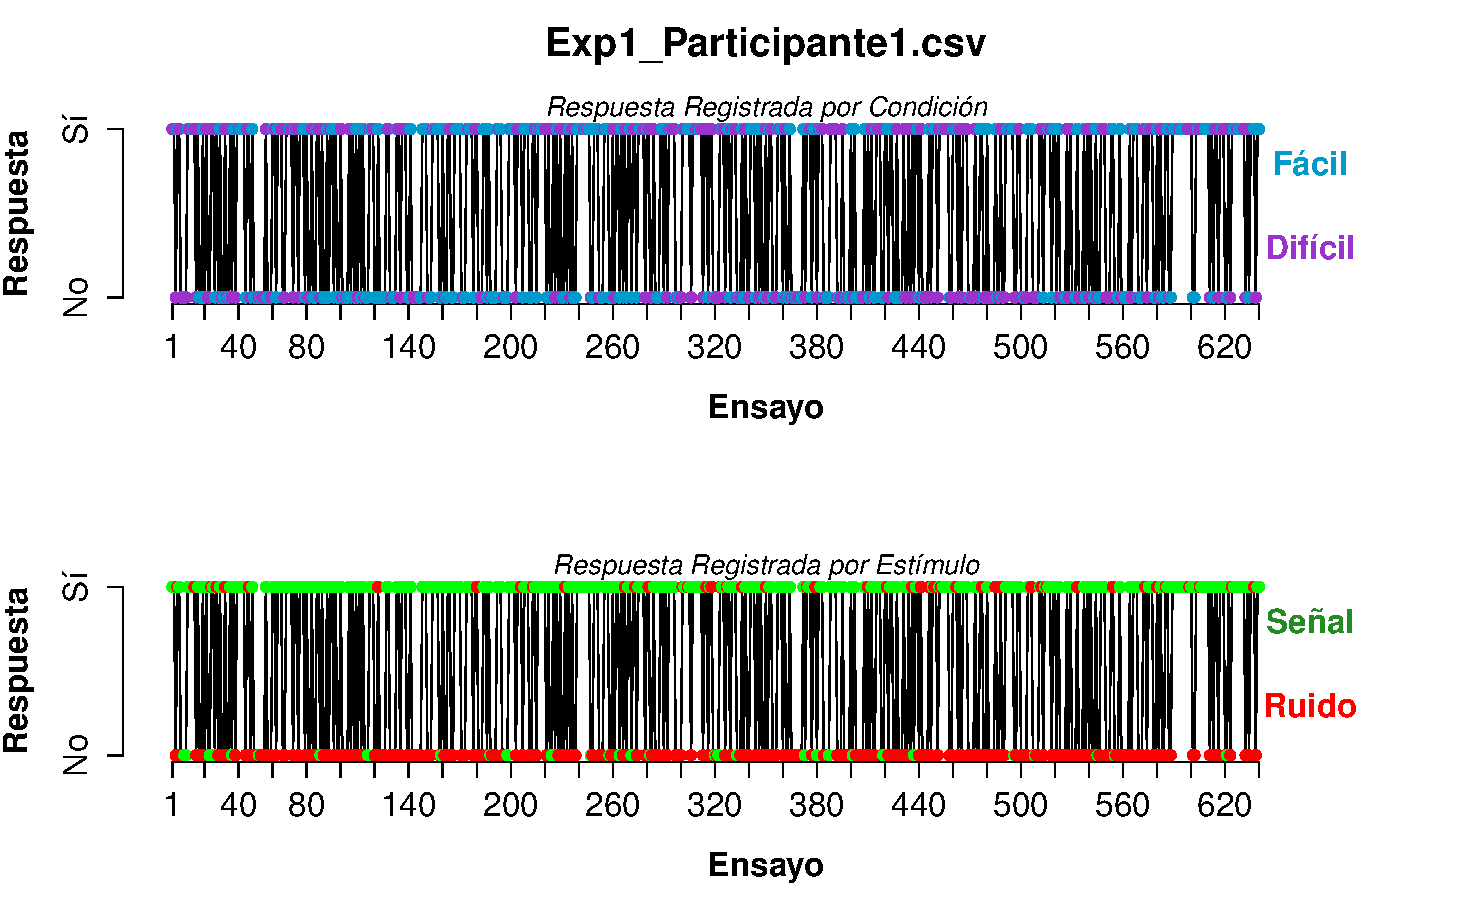
\includegraphics[width=0.60\textwidth]{Figures/BiasResp_Exp1_P1} 
%\decoRule
\caption[ParticipanteSesgado_Variables]{,}
\label{fig:BiasResp_E1_P1}
\end{figure}

Las Figuras~\ref{fig:BiasResp_E1} y () muestran las gráficas correspondientes al resto de los participantes en el Experimento 1 y 2, respectivamente.\\

\item Asignación de puntajes de confianza, ('1','2' y '3').

La segunda parte de la tarea de los participantes consistió en la asignación de un Puntaje de confianza que representara cuán seguros se sentían de la respuesta dada a la tarea principal. Un indicador de interés para determinar que los participantes respondieran a esta segunda tarea con atención fue el uso de todas las posibles opciones de respuesta. Por ello, realizamos un gráfico que identifica ensayo a ensayo, el puntaje de confianza asignado a la respuesta dada a cada uno de los estímulos evaluados. Durante la tarea, los participantes tenían que oprimir una tres posibles teclas ('1','2' y '3') para señalar qué tanta confianza tenían sobre su respuesta previa ('poco seguro', 'más o menos seguro' o 'muy seguro', respectivamente), respuestas que posteriormente el programa traduciría a una escala más larga, con valores del 1 al 6, que permite distinguir entre la confianza de haber rechazado correctamente un estímulo con ruido (e.g. '1, estoy seguro de que los círculos eran diferentes') y haber acertado en la detección de los casos de interes (e.g '6, estoy seguro de que los círculos son iguales'), dejando los valores intermedios de la escala para los puntajes de poca confianza (e.g. '3, poco seguro de que los círculos eran diferentes' y '4, poco seguro de que los círculos son iguales').\\


\begin{figure}[th]
\centering
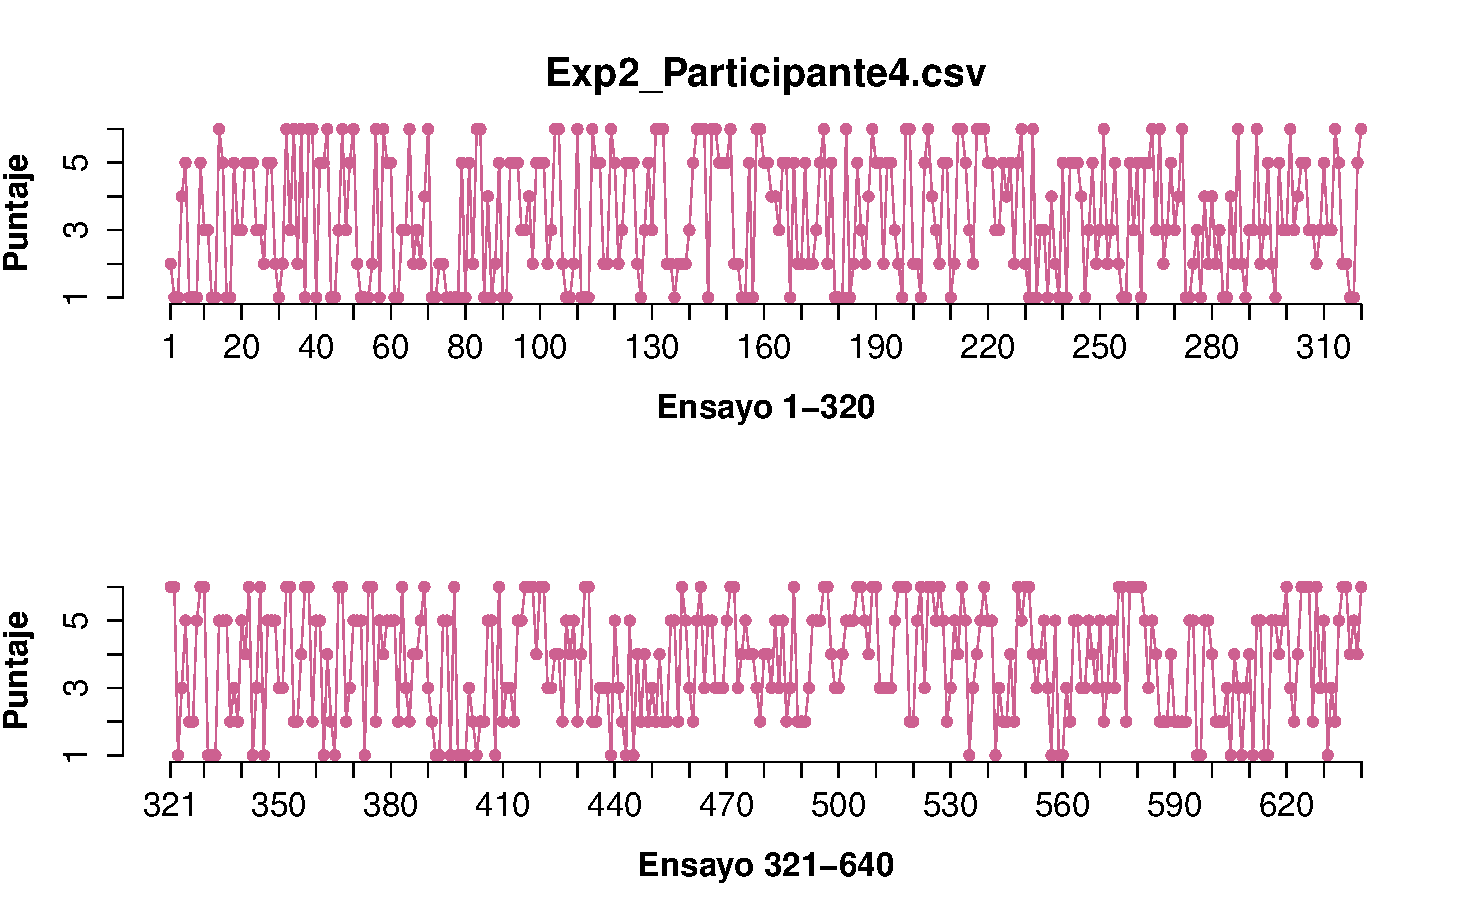
\includegraphics[width=0.50\textwidth]{Figures/Rating_Exp2_P4} 
%\decoRule
\caption[Asignacion Puntaje de confianza: Participante con multiples elecciones]{,}
\label{fig:Rating_E2_P4}
\end{figure}

La Figura~\ref{fig:Rating_E2_P4} muestra los puntajes emitidos por el Participante 4 del Experimento 2 a lo largo de los 640 ensayos que componen la tarea, sirviéndonos como un ejemplo de variabilidad en el uso de todas las opciones de respuesta. Debido a la conversión que el programa realizó sobre las respuestas emitidas para obtener puntajes en un intervalo de confianza, este tipo de gráfico nos permite evaluar el uso de todas las teclas de respuesta (i.e. puntajes de 3 y 4, señalan el uso de la tecla 1; 2 y 5, la tecla 2 y 1 y 6, la tecla 3) e informarnos simultáneamente sobre la respuesta que el participante emitió previamente en la tarea de detección binaria.

.Los gráficos correspondientes a los participantes restantes en los Experimentos 1 y 2, se muestran en las Figuras~\ref{fig:Rating_E2}, respectivamente.\\

\end{itemize}

\begin{figure}[th]
\centering
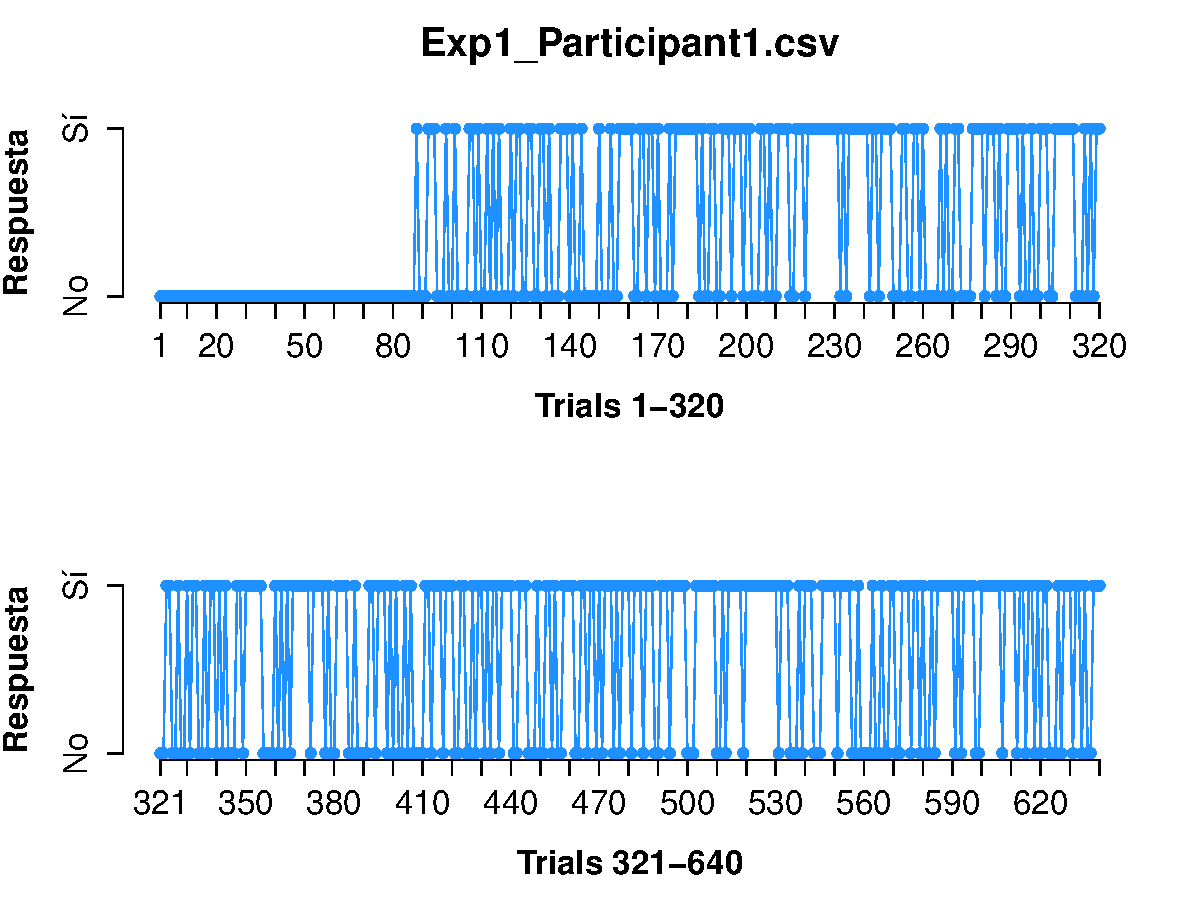
\includegraphics[width=0.30\textwidth]{Figures/Response_Exp1_P1} 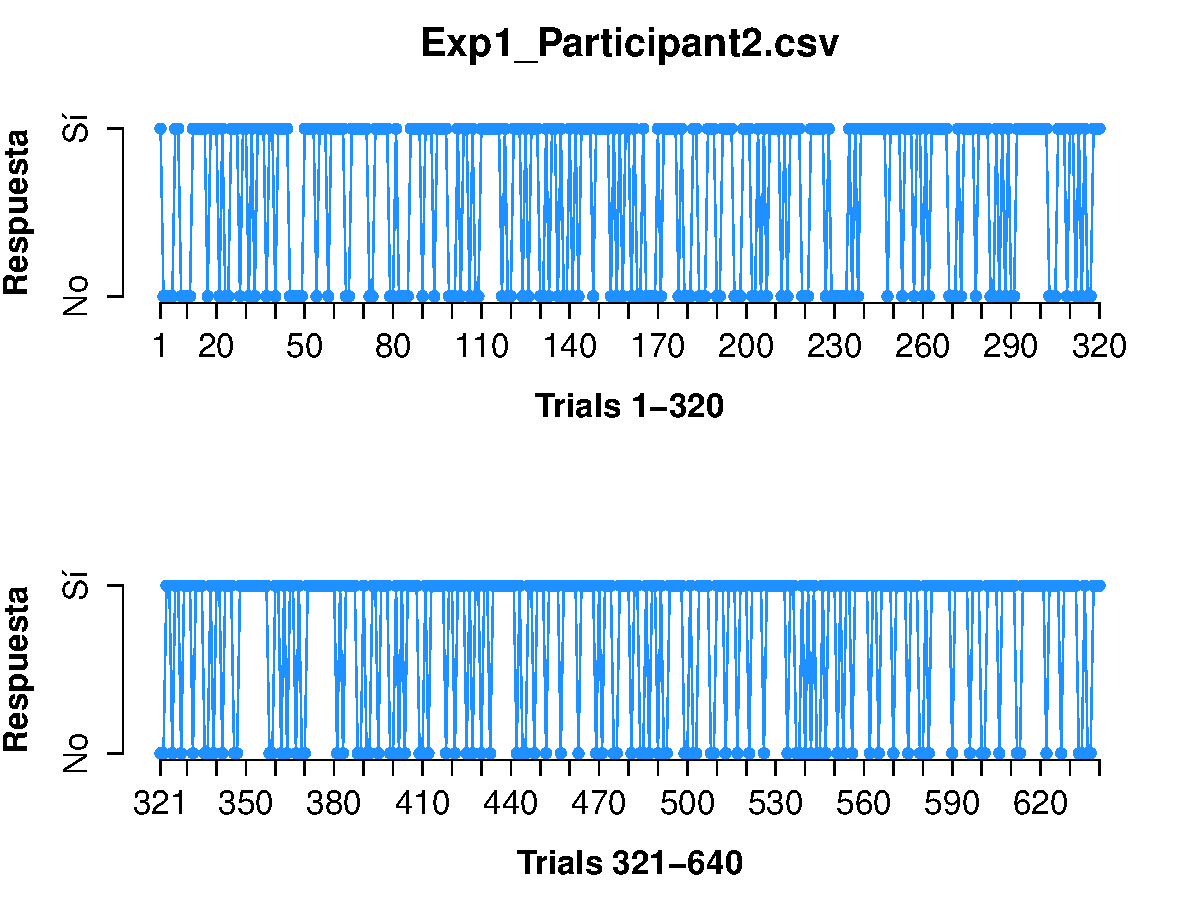
\includegraphics[width=0.30\textwidth]{Figures/Response_Exp1_P2} 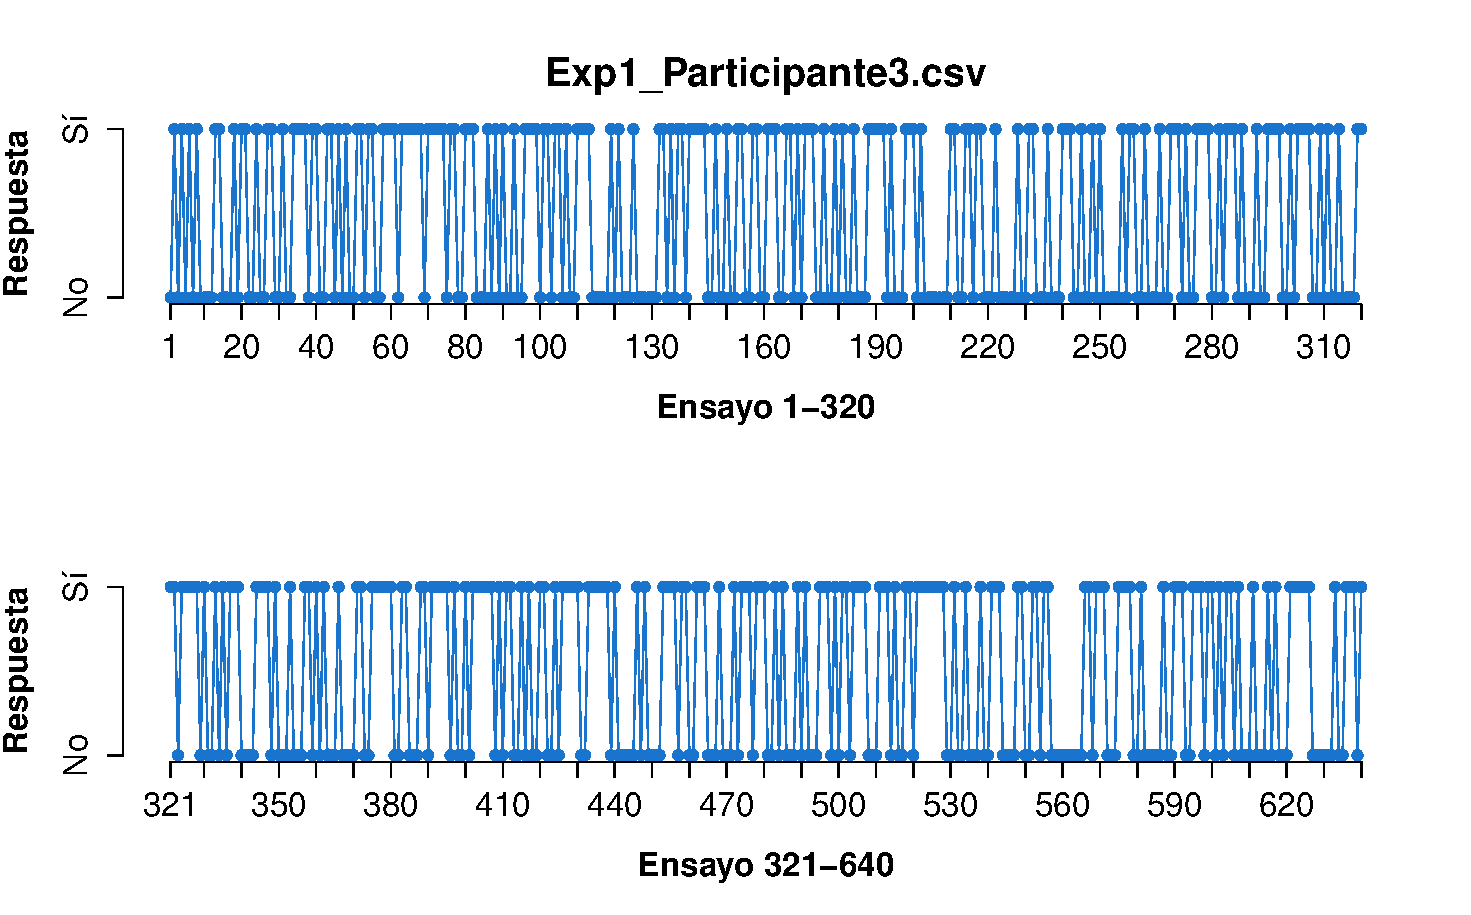
\includegraphics[width=0.30\textwidth]{Figures/Response_Exp1_P3}
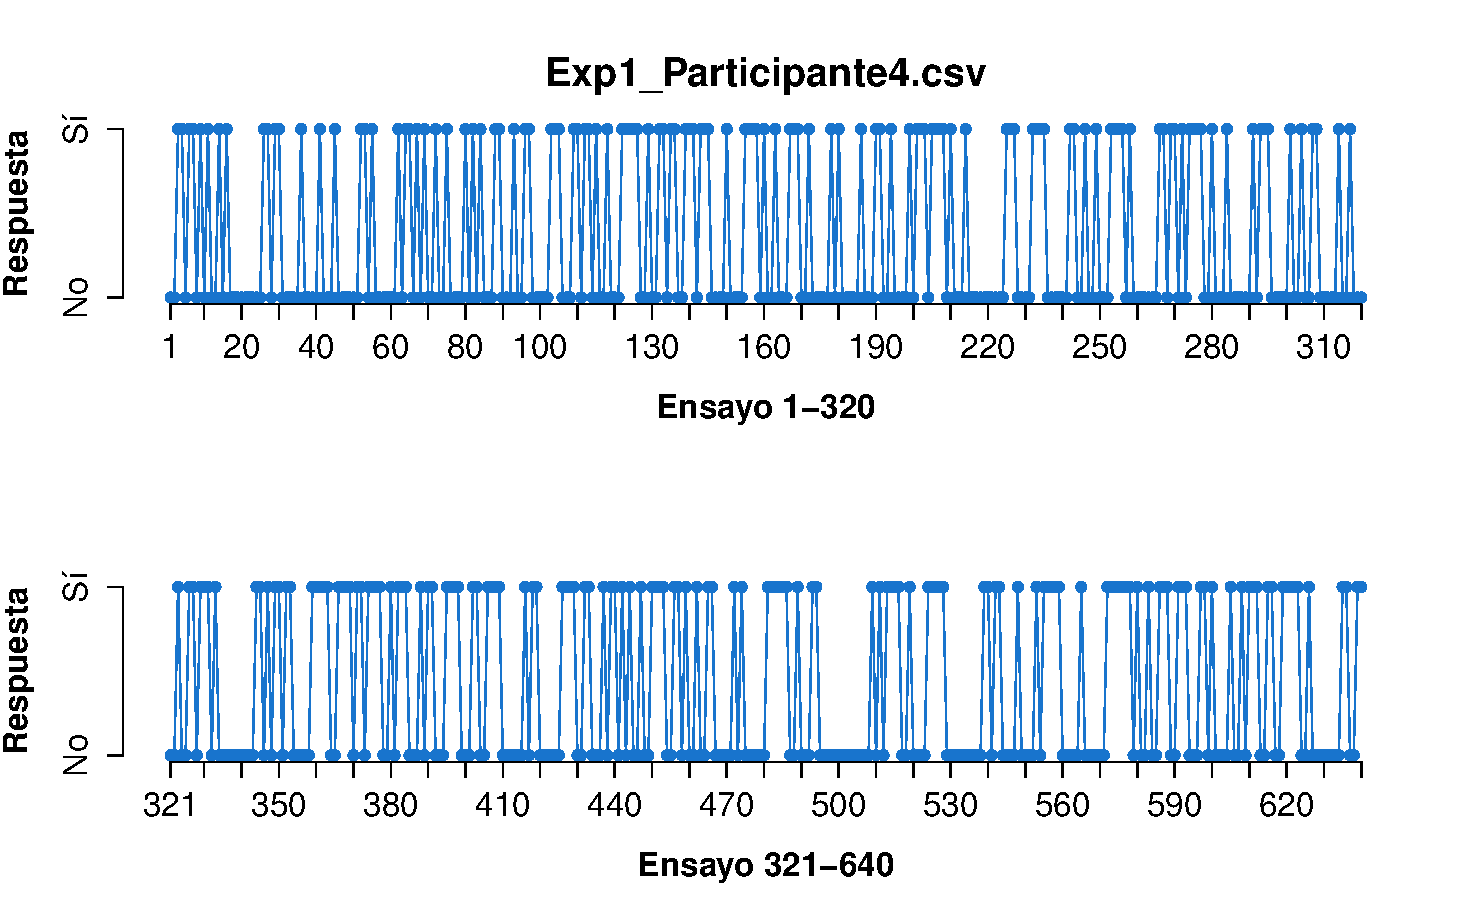
\includegraphics[width=0.30\textwidth]{Figures/Response_Exp1_P4} 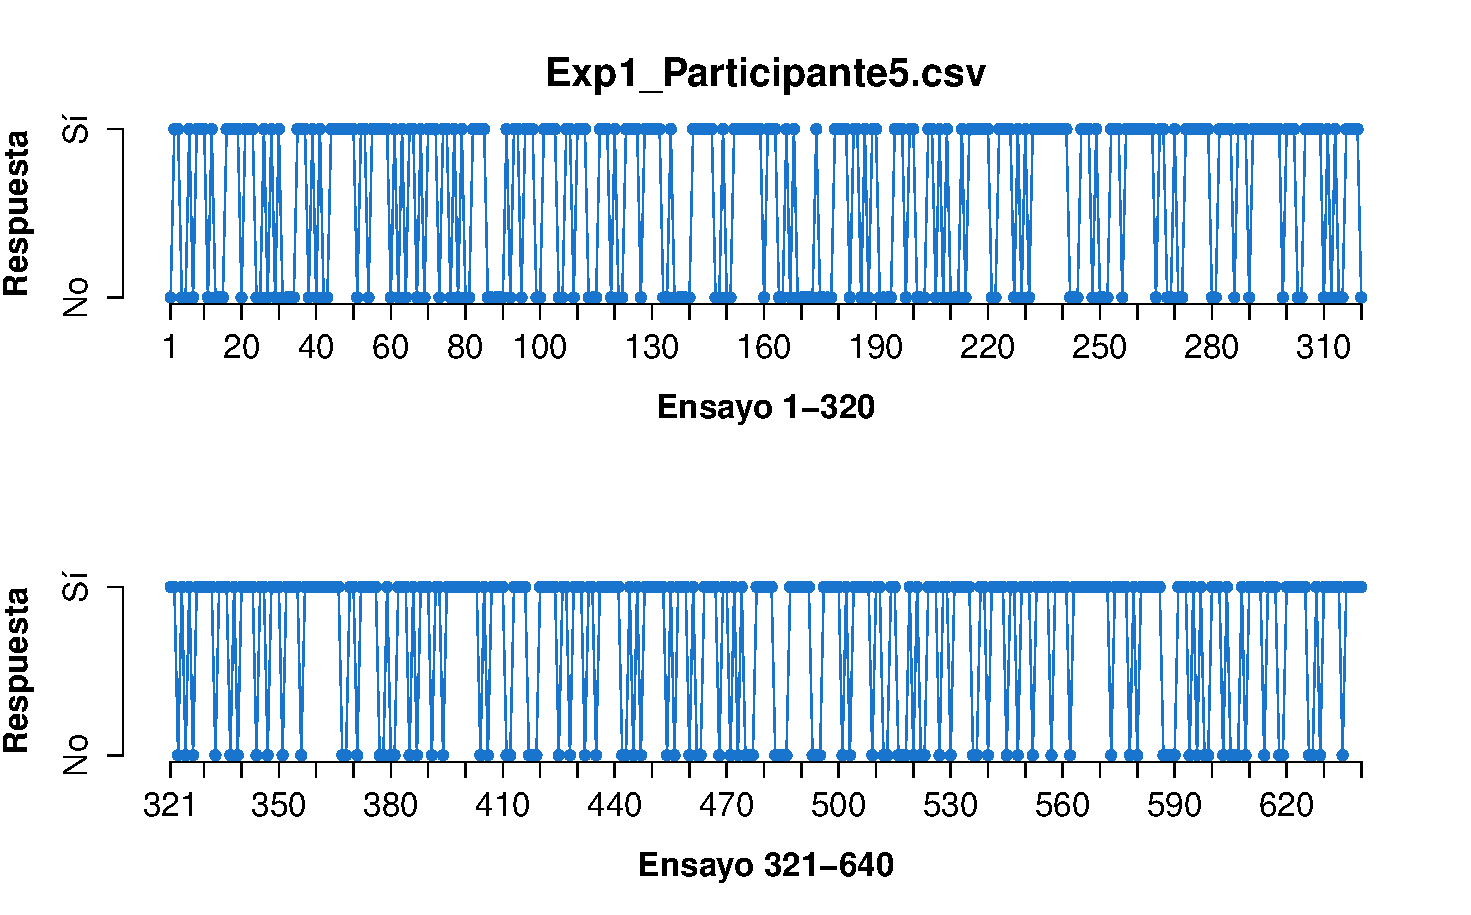
\includegraphics[width=0.30\textwidth]{Figures/Response_Exp1_P5} 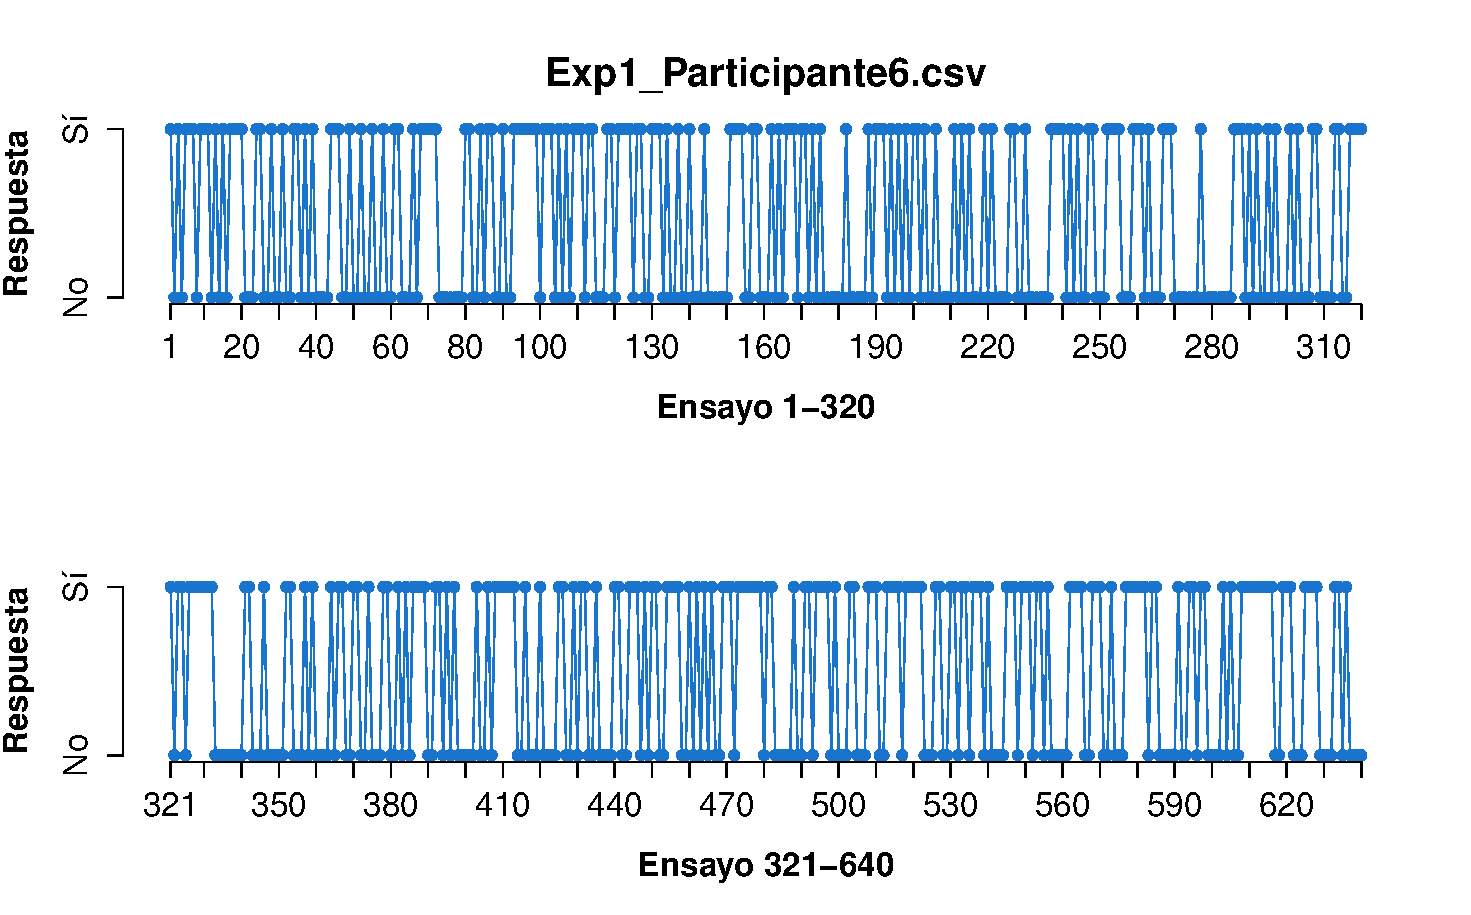
\includegraphics[width=0.30\textwidth]{Figures/Response_Exp1_P6}
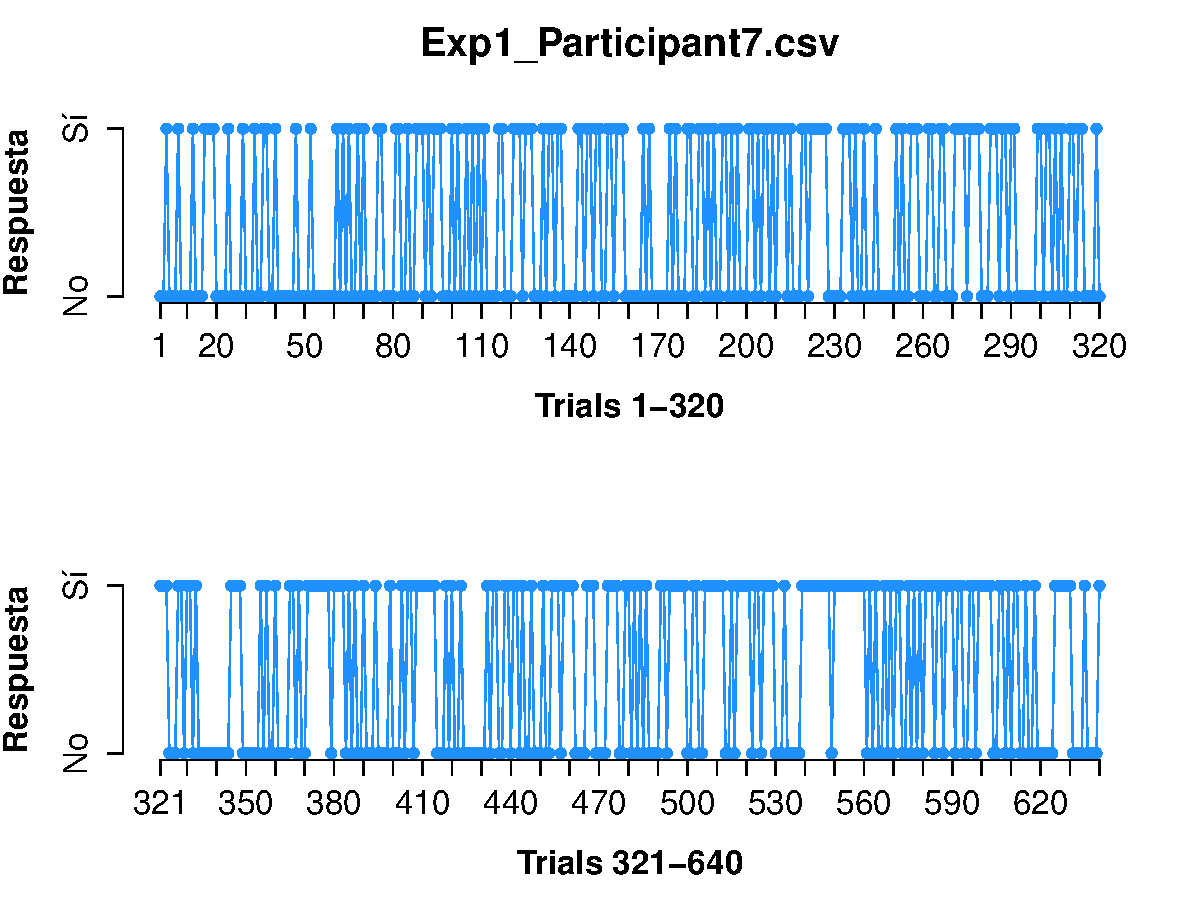
\includegraphics[width=0.30\textwidth]{Figures/Response_Exp1_P7} 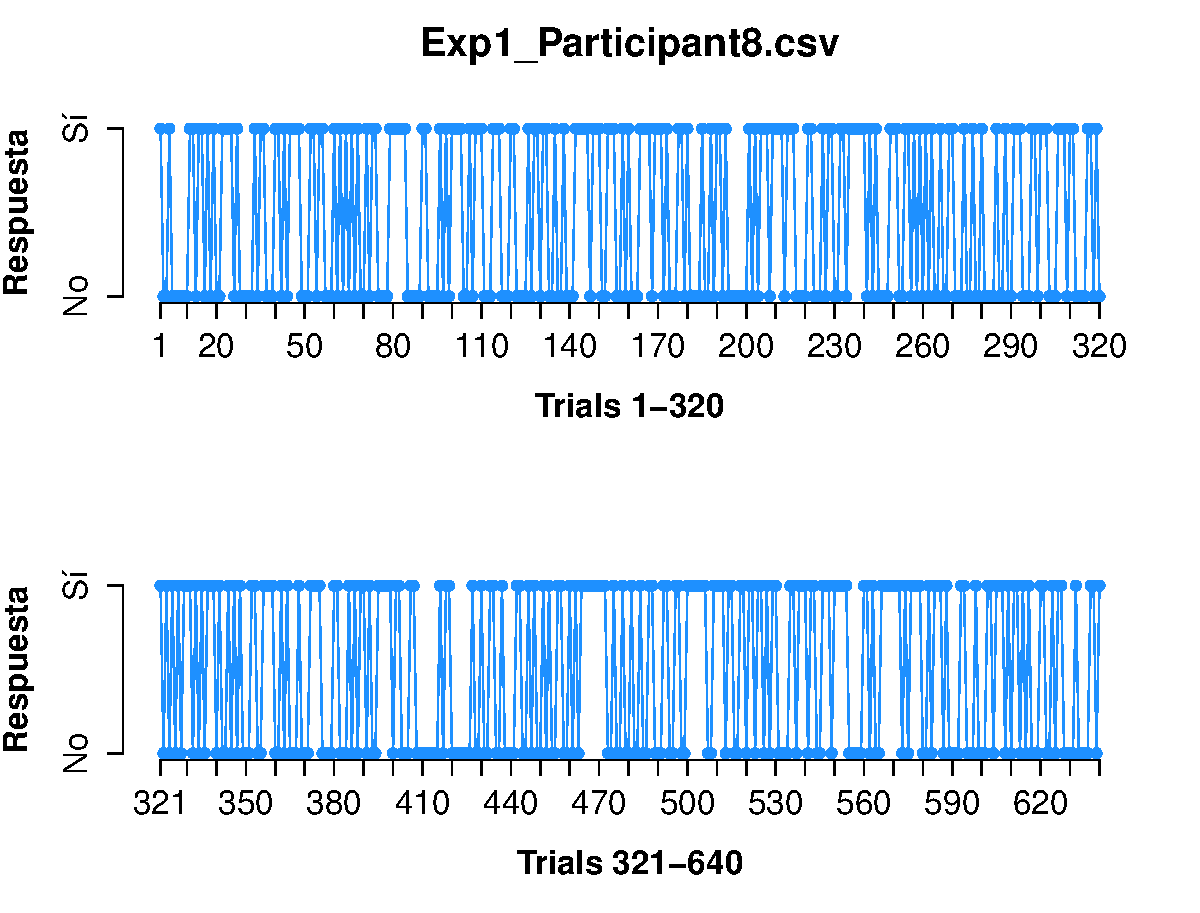
\includegraphics[width=0.30\textwidth]{Figures/Response_Exp1_P8} 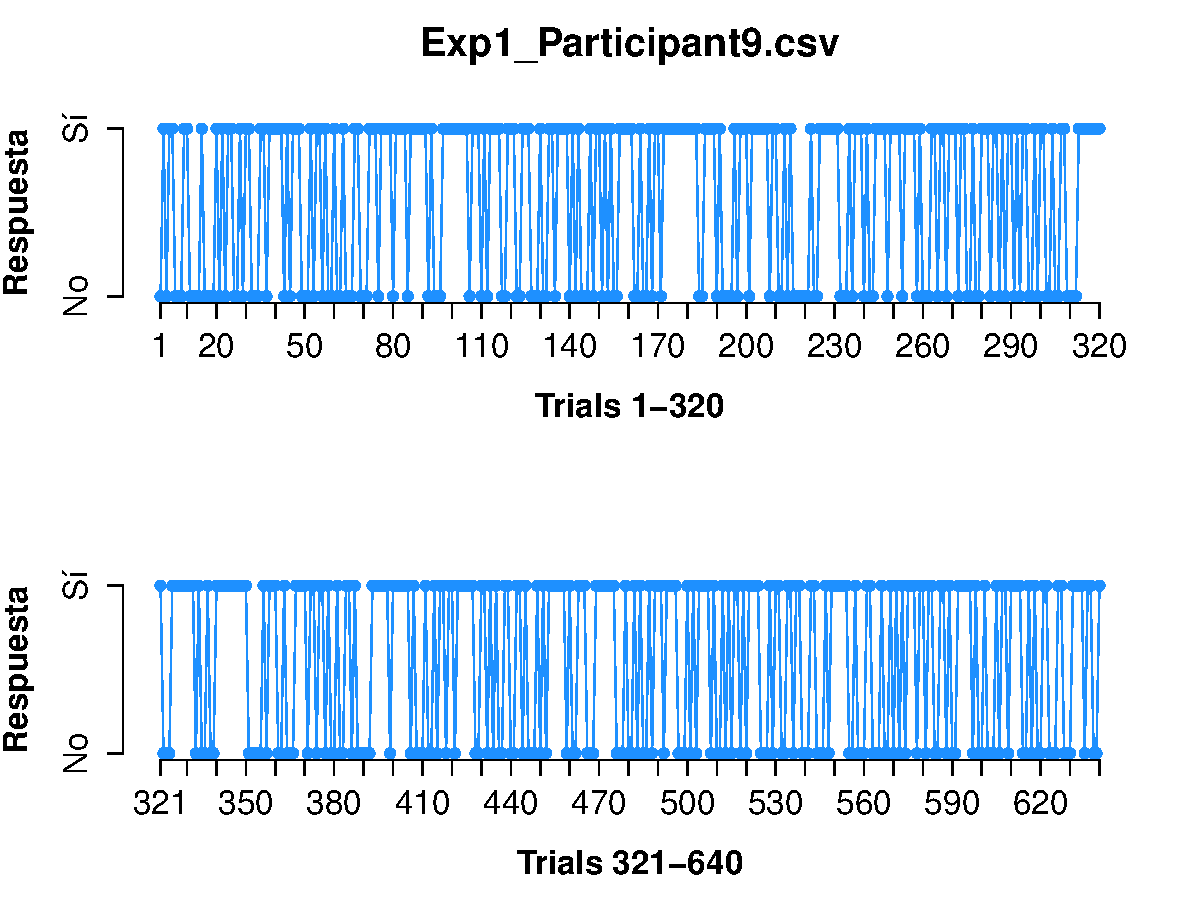
\includegraphics[width=0.30\textwidth]{Figures/Response_Exp1_P9}
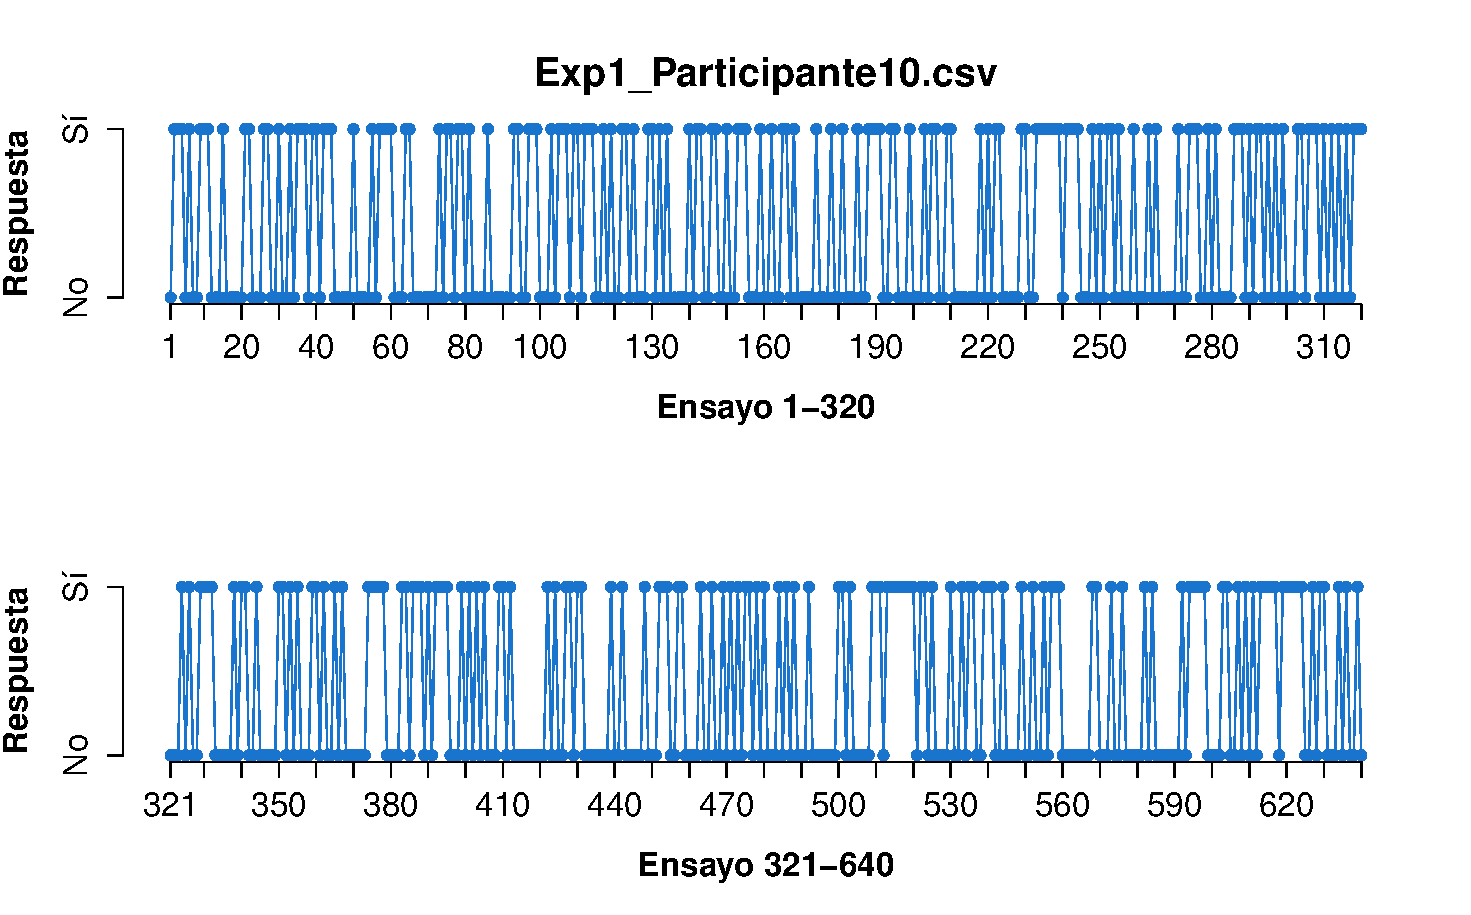
\includegraphics[width=0.30\textwidth]{Figures/Response_Exp1_P10} 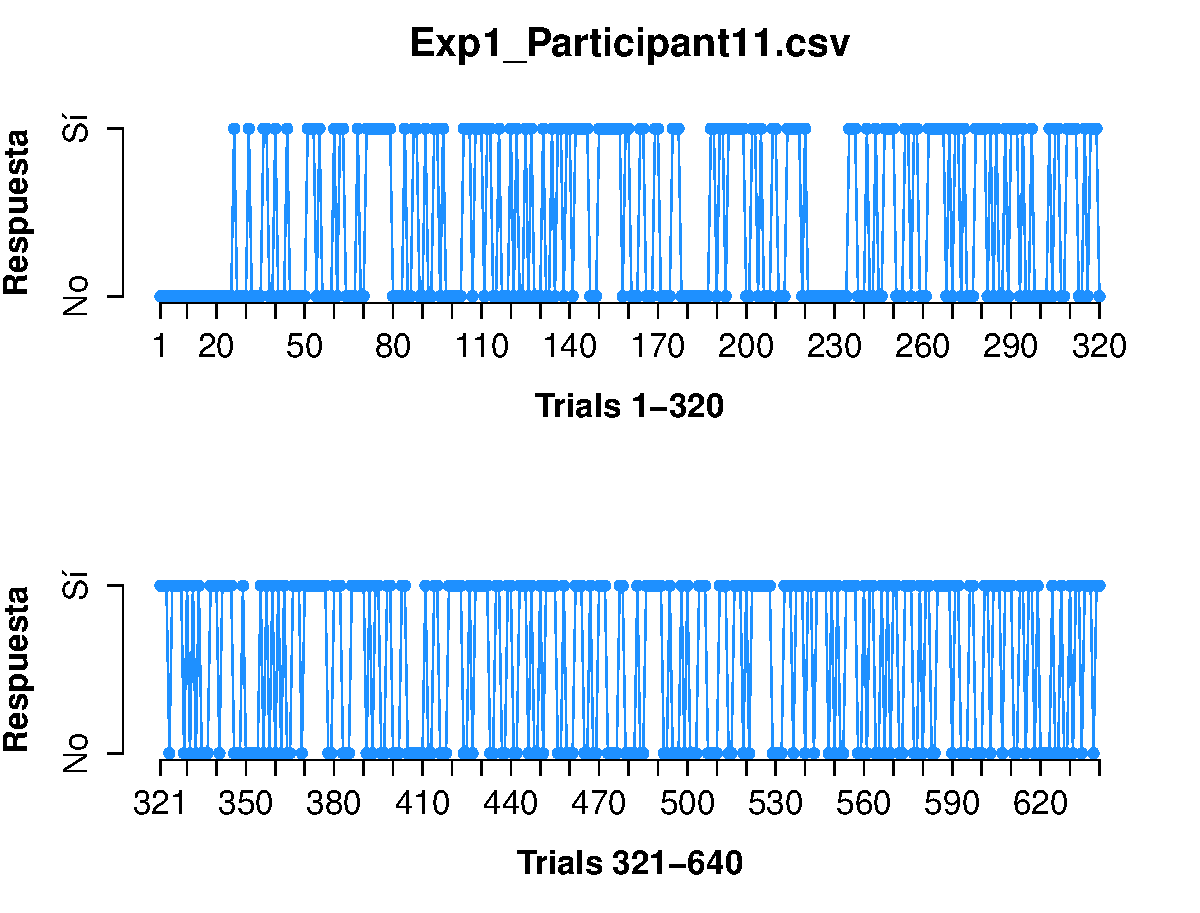
\includegraphics[width=0.30\textwidth]{Figures/Response_Exp1_P11} 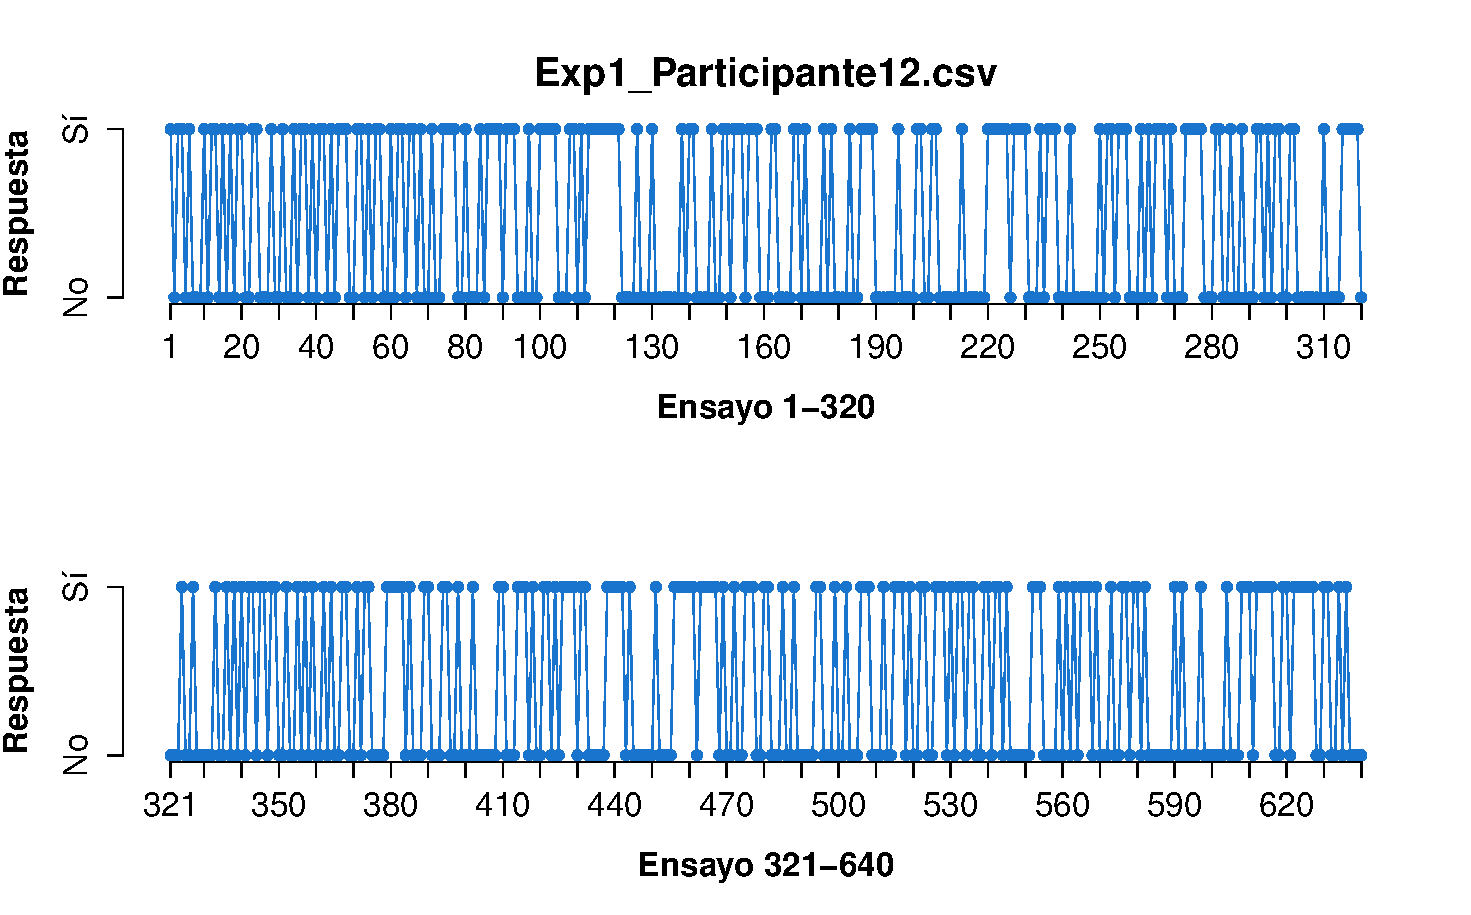
\includegraphics[width=0.30\textwidth]{Figures/Response_Exp1_P12}
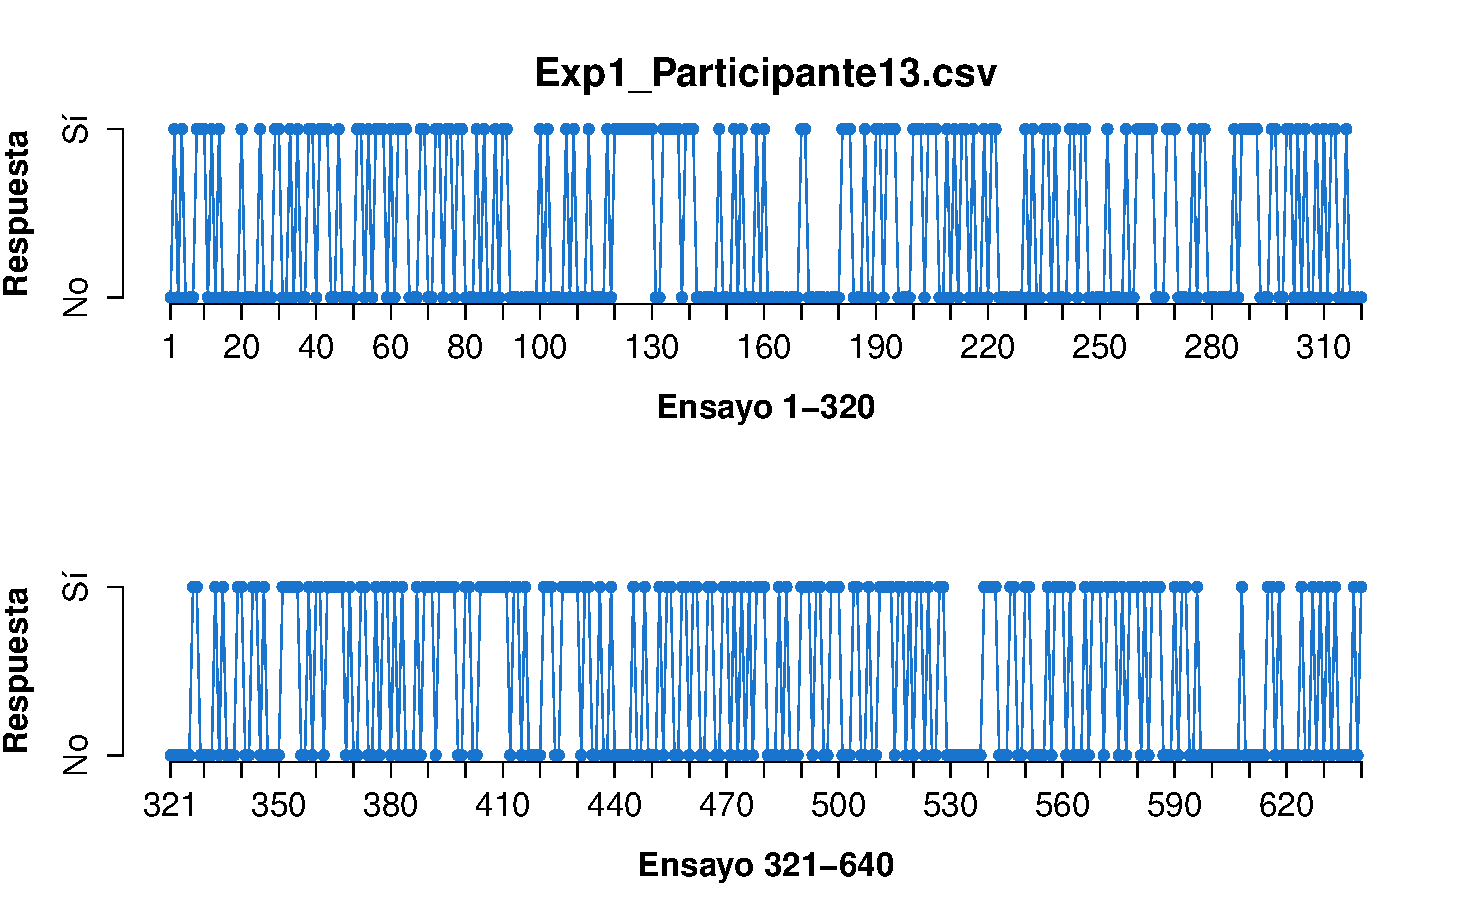
\includegraphics[width=0.30\textwidth]{Figures/Response_Exp1_P13} 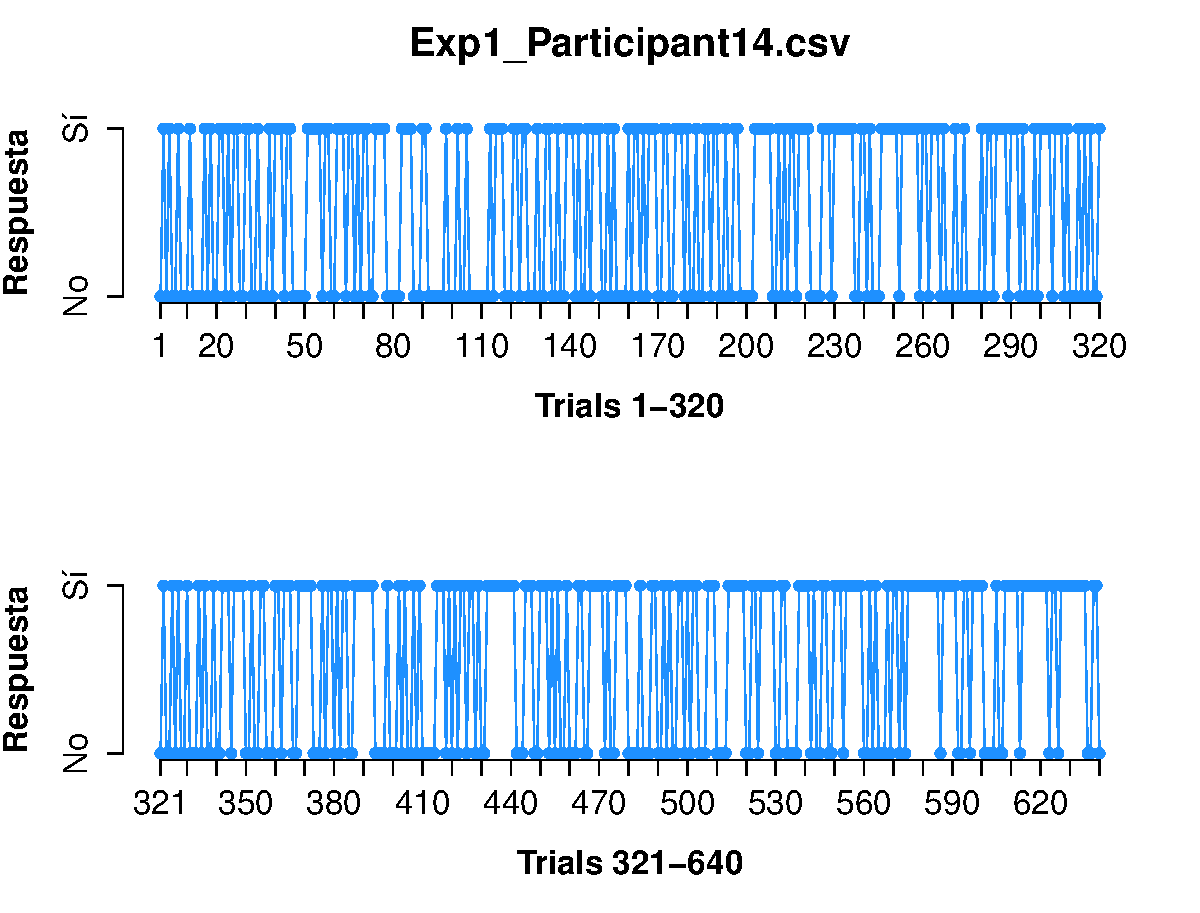
\includegraphics[width=0.30\textwidth]{Figures/Response_Exp1_P14} 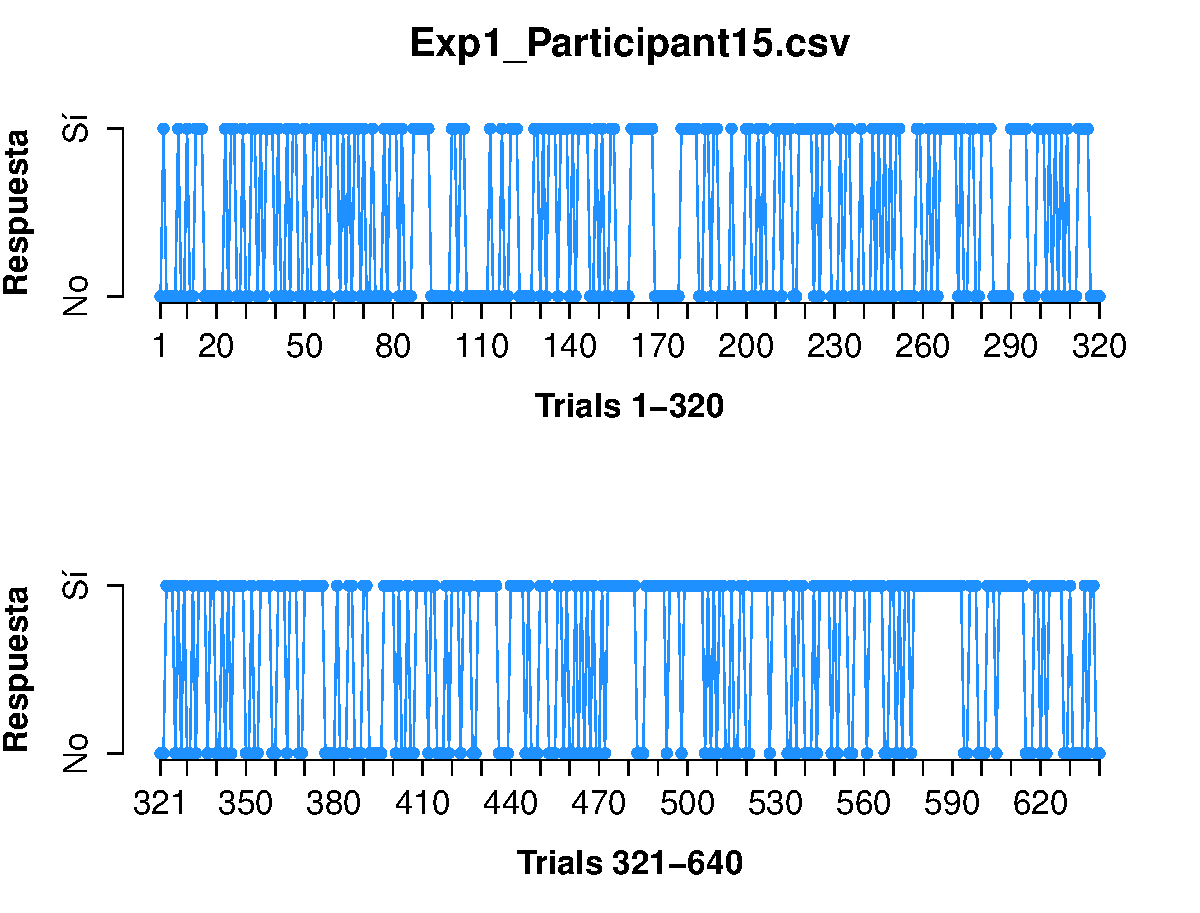
\includegraphics[width=0.30\textwidth]{Figures/Response_Exp1_P15}
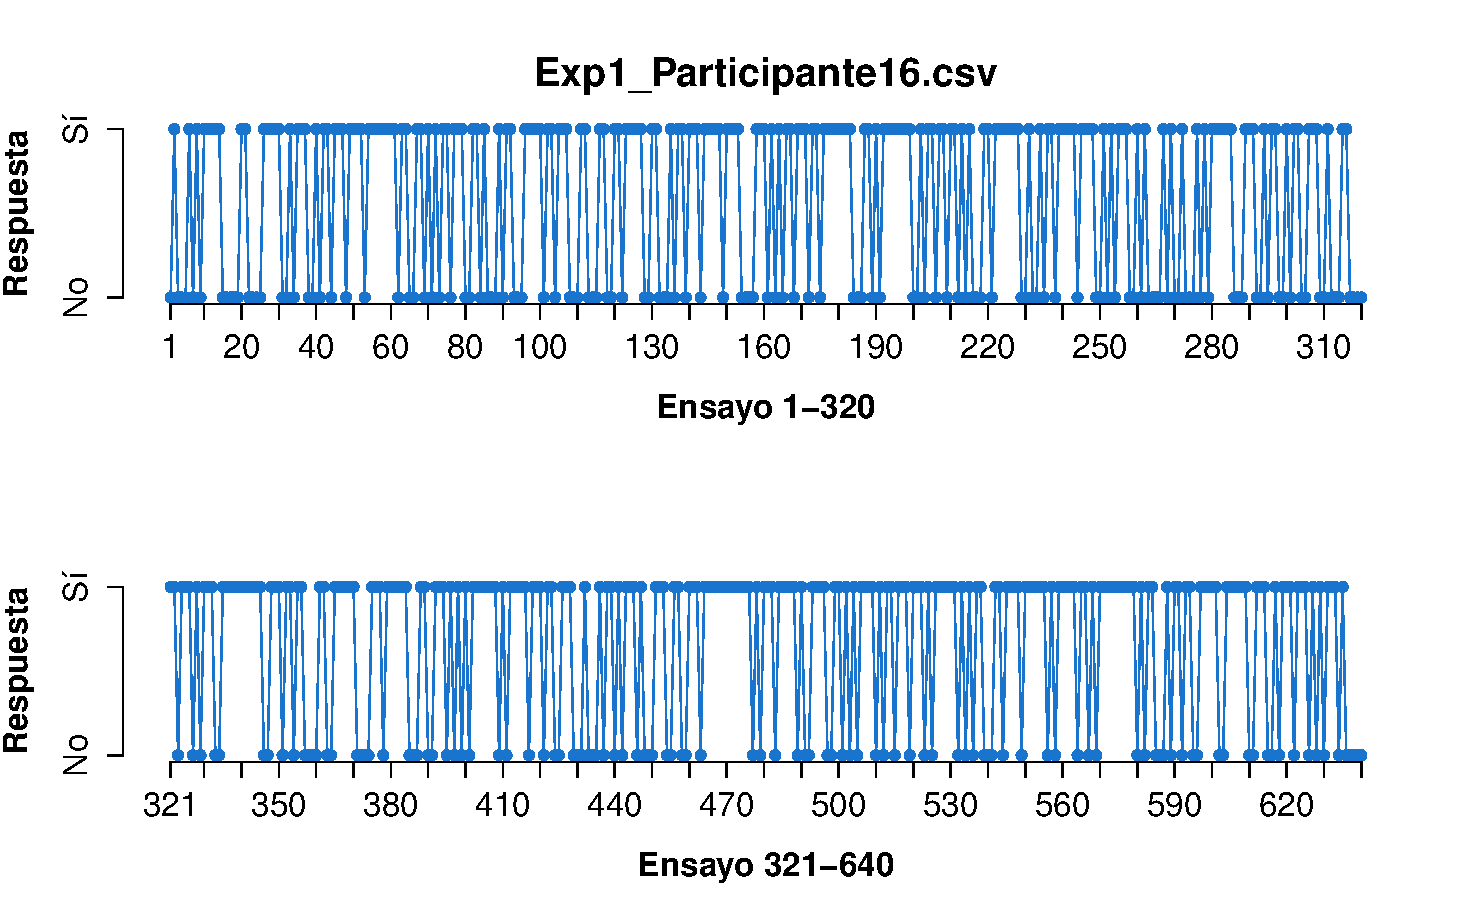
\includegraphics[width=0.30\textwidth]{Figures/Response_Exp1_P16} 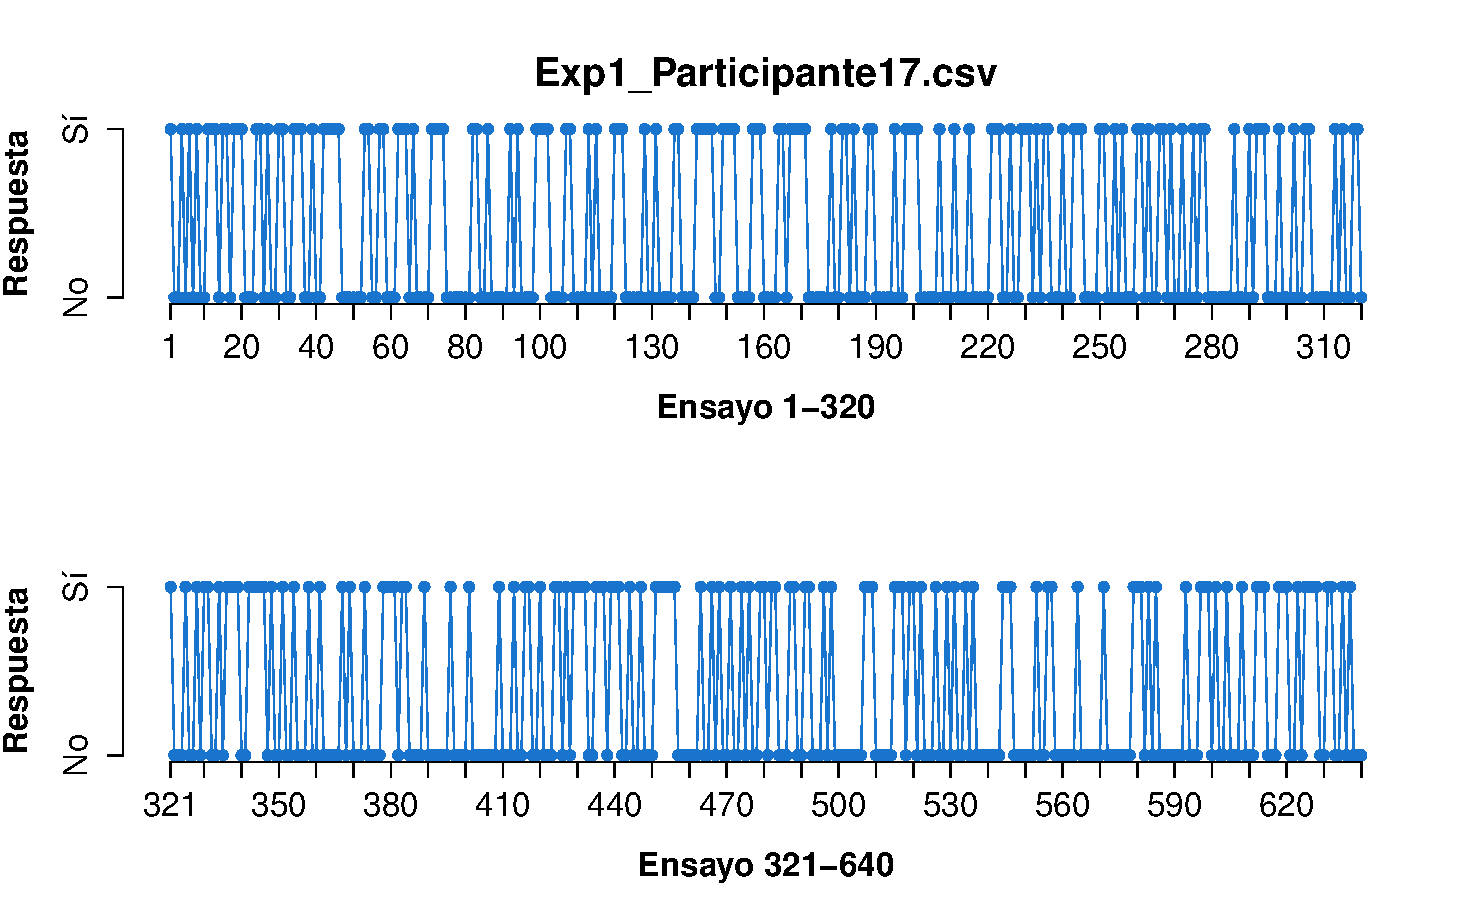
\includegraphics[width=0.30\textwidth]{Figures/Response_Exp1_P17} 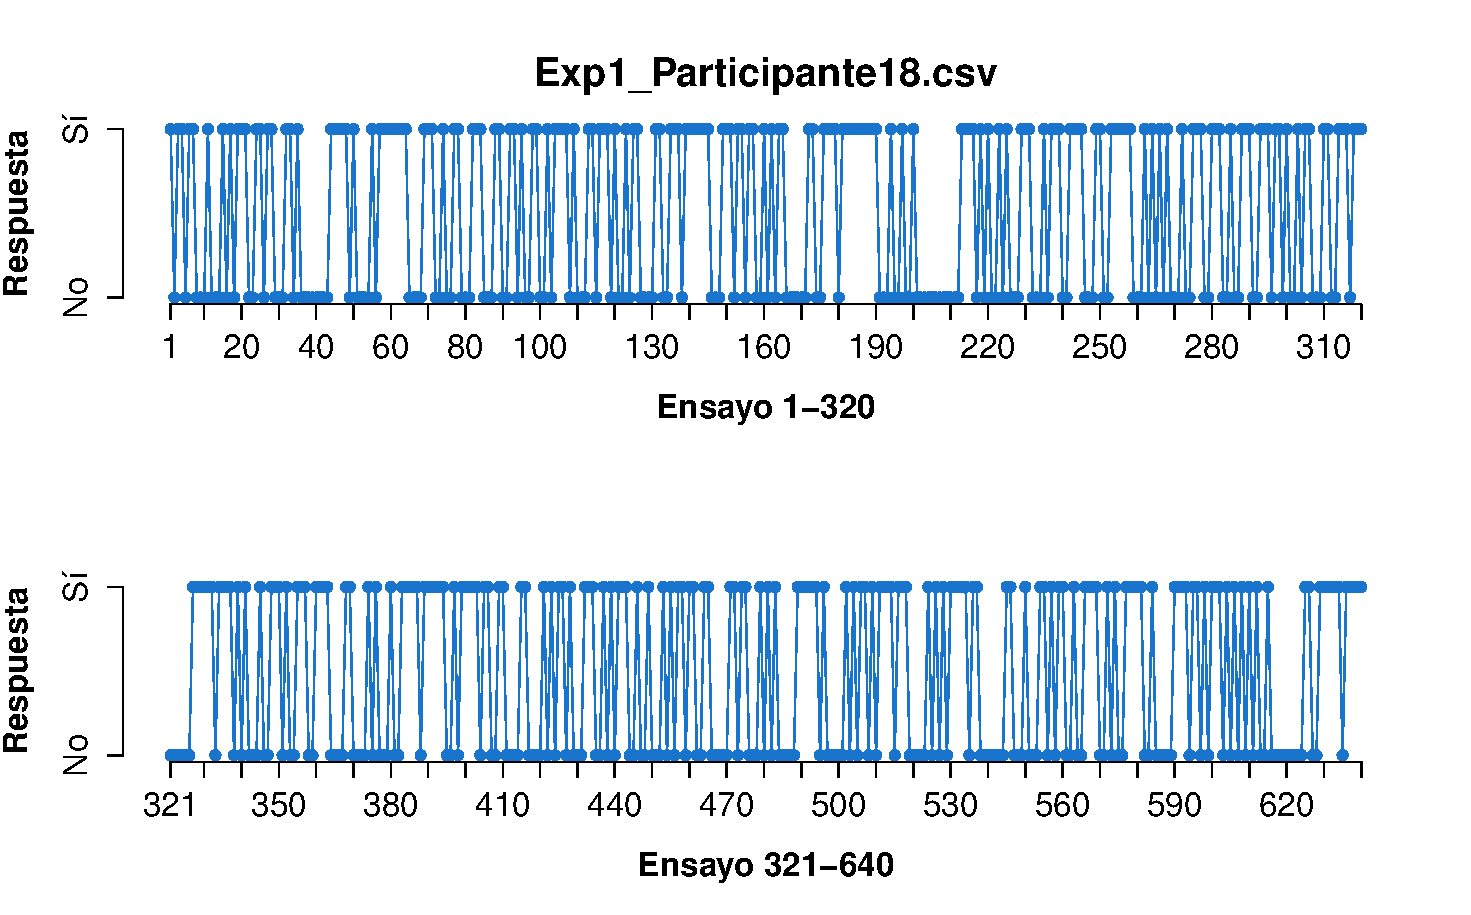
\includegraphics[width=0.30\textwidth]{Figures/Response_Exp1_P18}
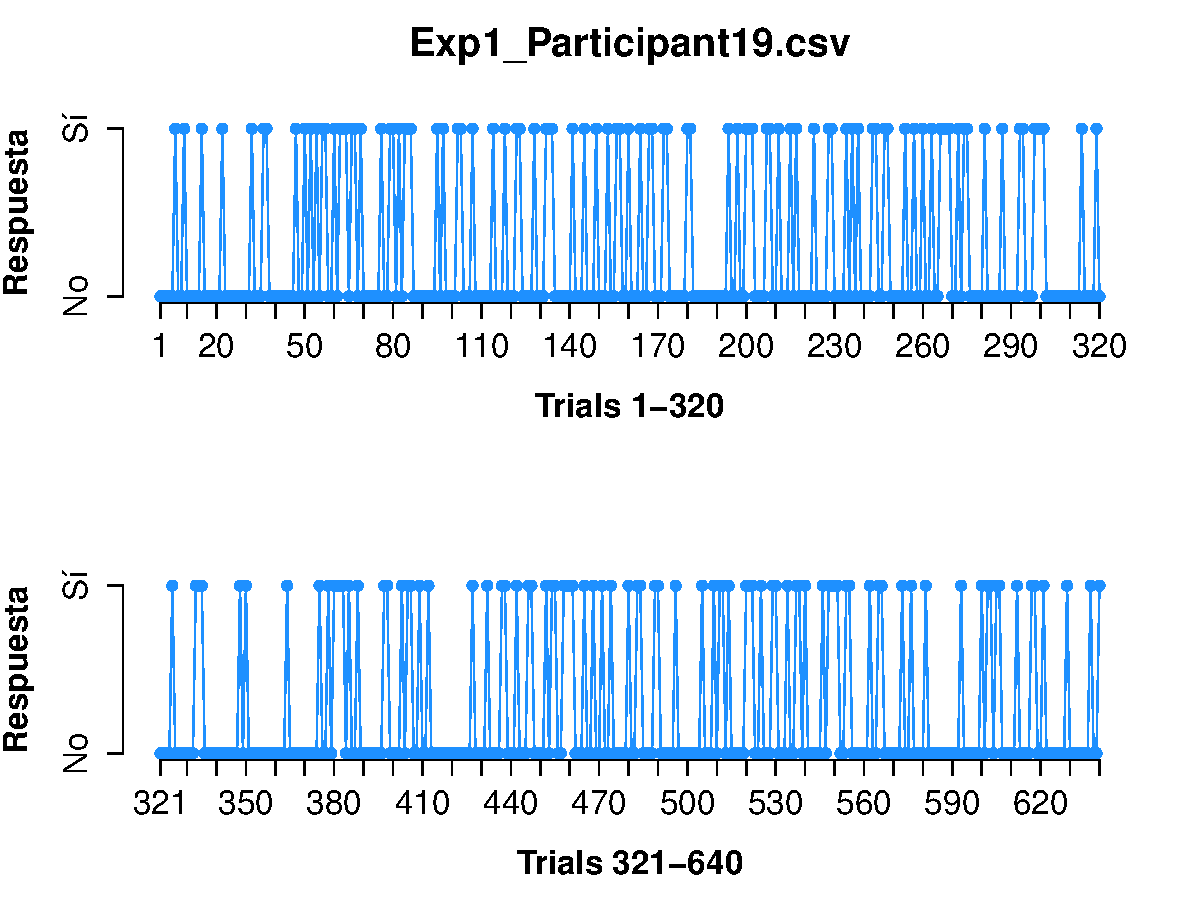
\includegraphics[width=0.30\textwidth]{Figures/Response_Exp1_P19} 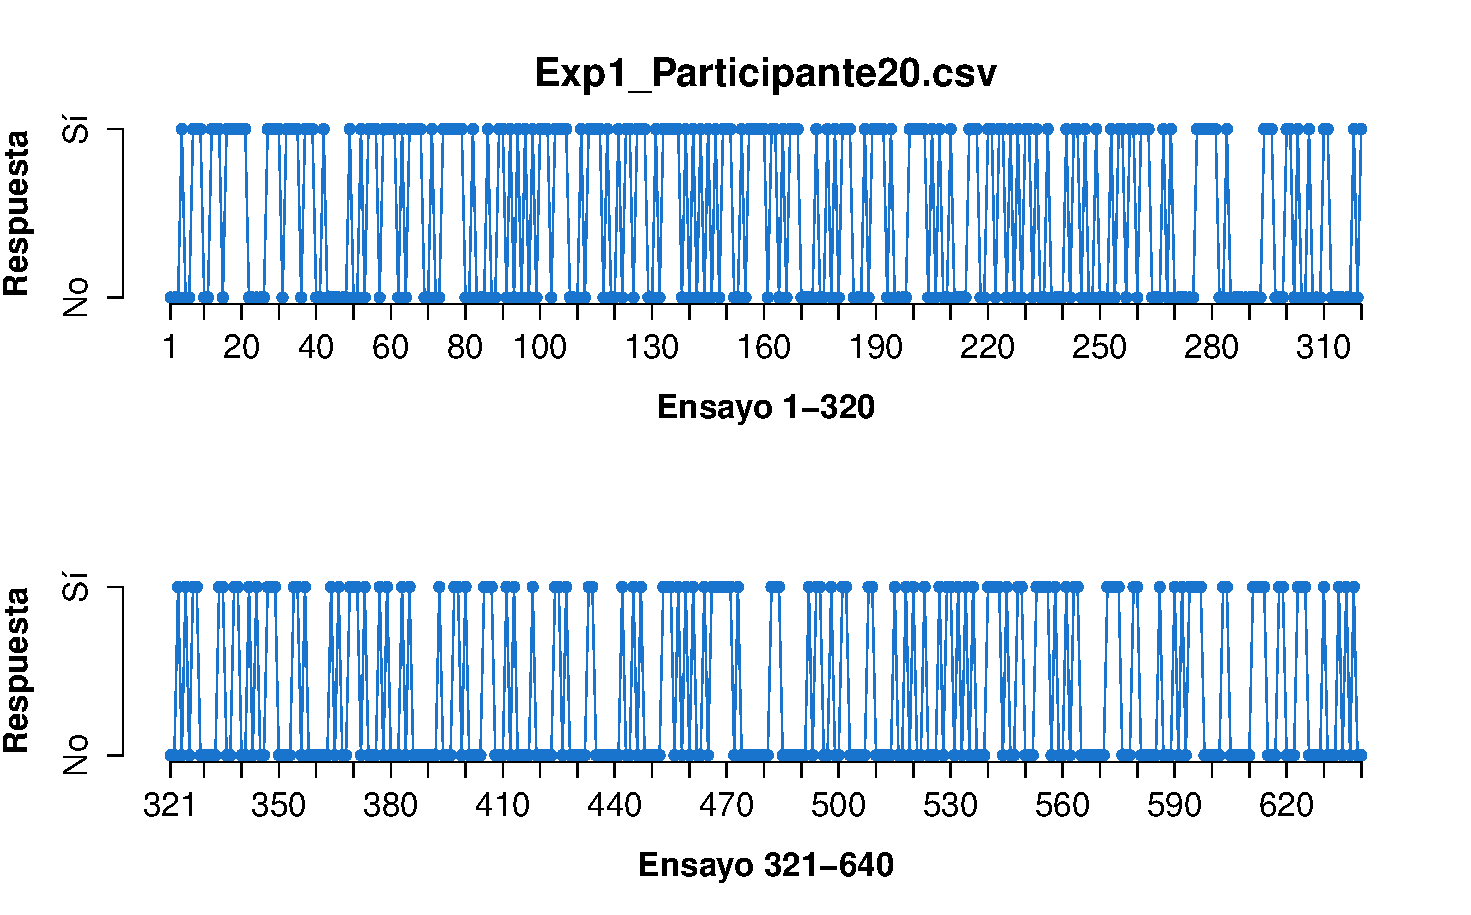
\includegraphics[width=0.30\textwidth]{Figures/Response_Exp1_P20} 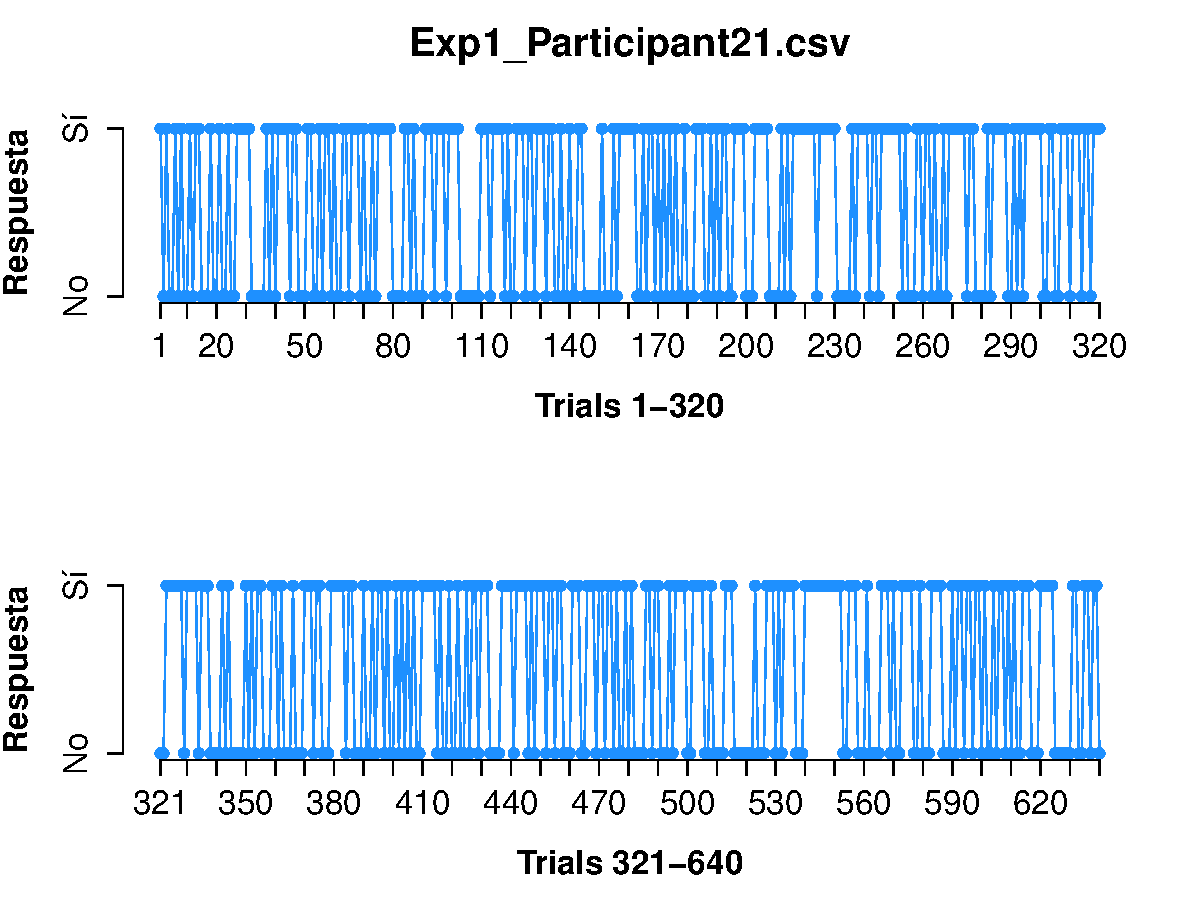
\includegraphics[width=0.30\textwidth]{Figures/Response_Exp1_P21} 
%\decoRule
\caption[Response_Exp1]{Respuesta registrada, ensayo a ensayo, durante la tarea de detección binaria por cada uno de los veintiun paticipantes del Experimento 1. Por cada participante, se presentan dos gráficas que ilustran las elecciones realizadas durante la primera y la segunda mitad del experimento, (panel superior e inferior, respectivamente).}
\label{fig:Response_E1}
\end{figure}

\begin{figure}[th]
\centering
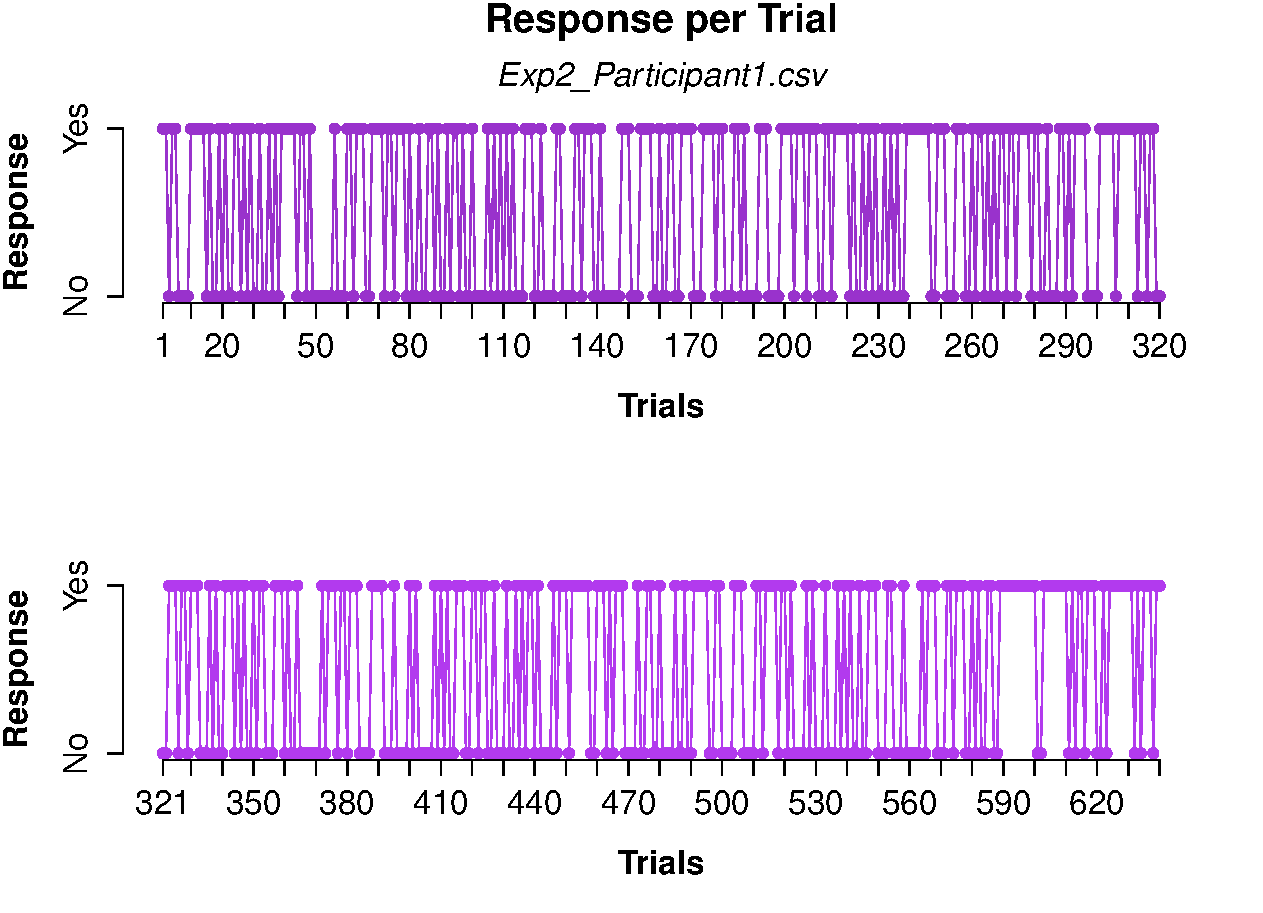
\includegraphics[width=0.30\textwidth]{Figures/Response_Exp2_P1} 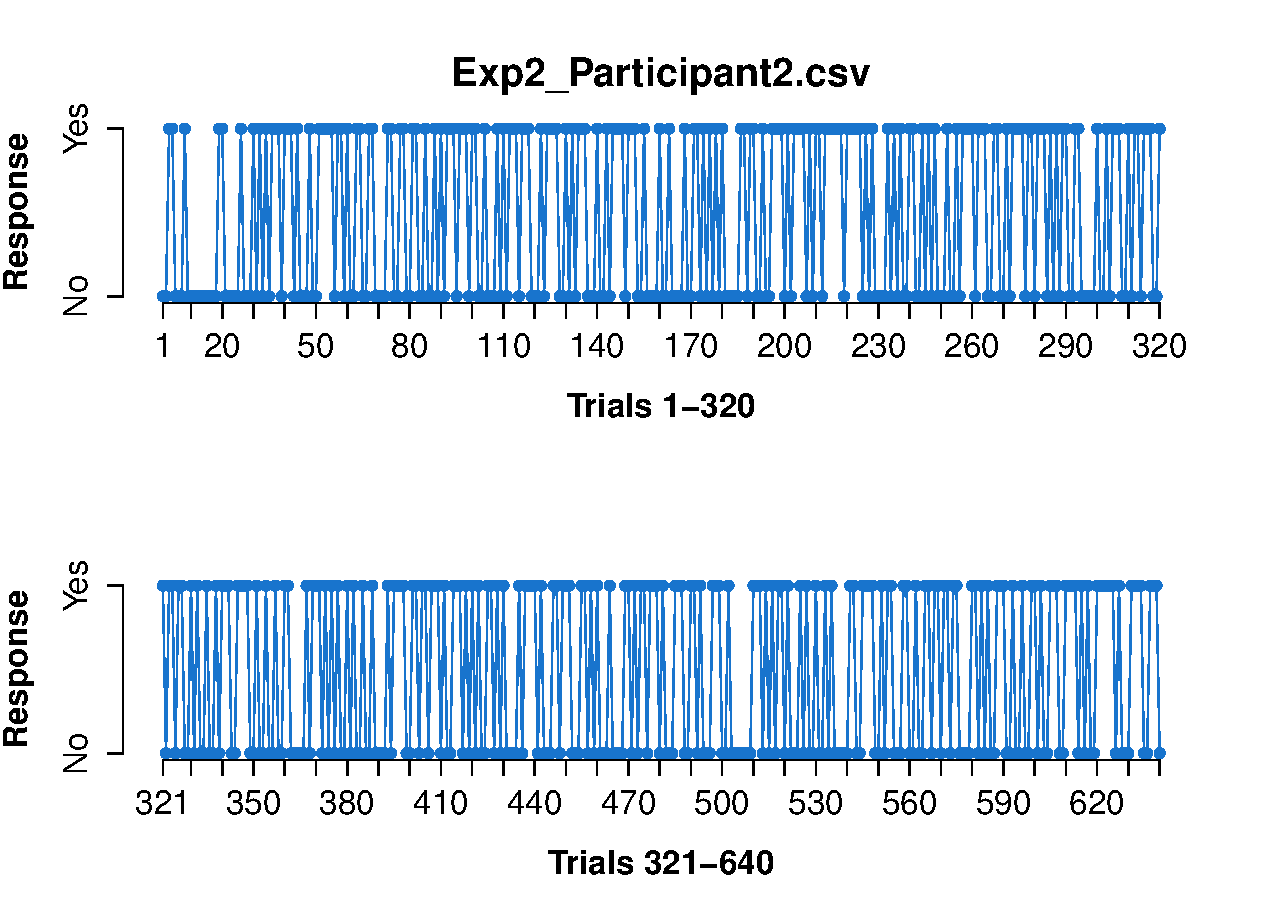
\includegraphics[width=0.30\textwidth]{Figures/Response_Exp2_P2} 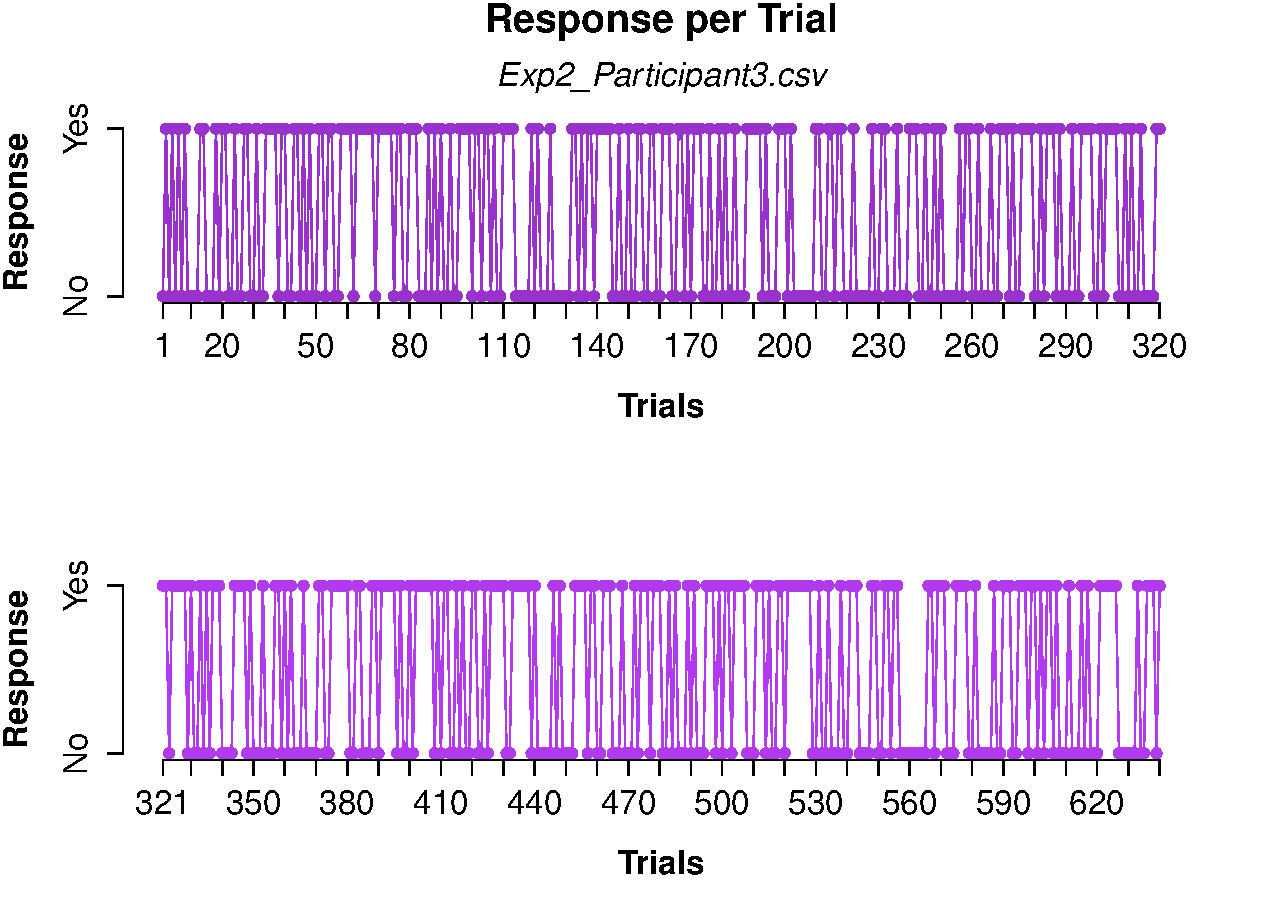
\includegraphics[width=0.30\textwidth]{Figures/Response_Exp2_P3}
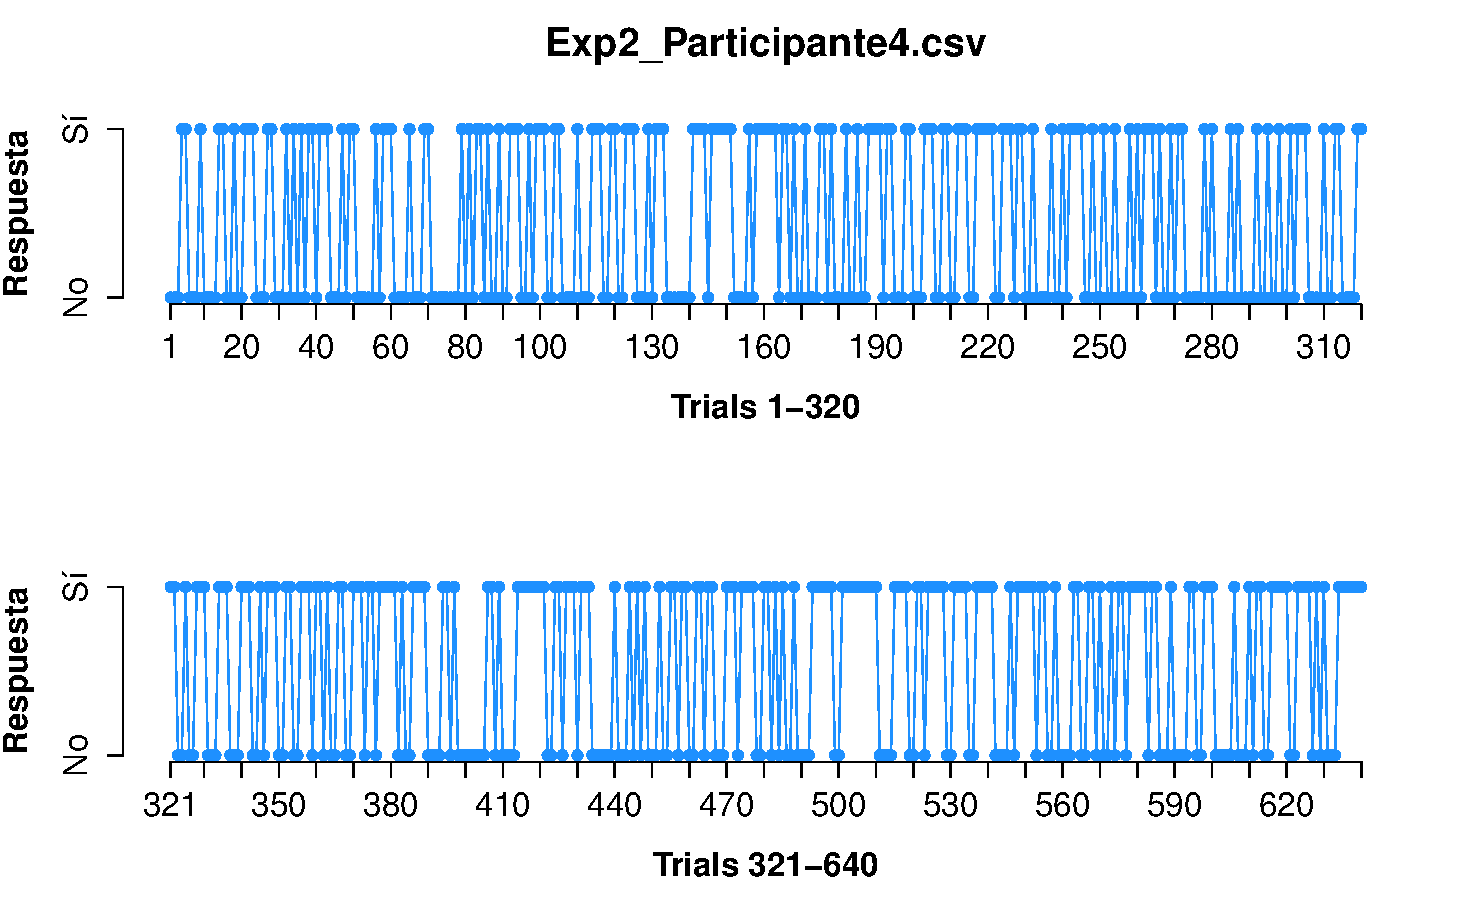
\includegraphics[width=0.30\textwidth]{Figures/Response_Exp2_P4} 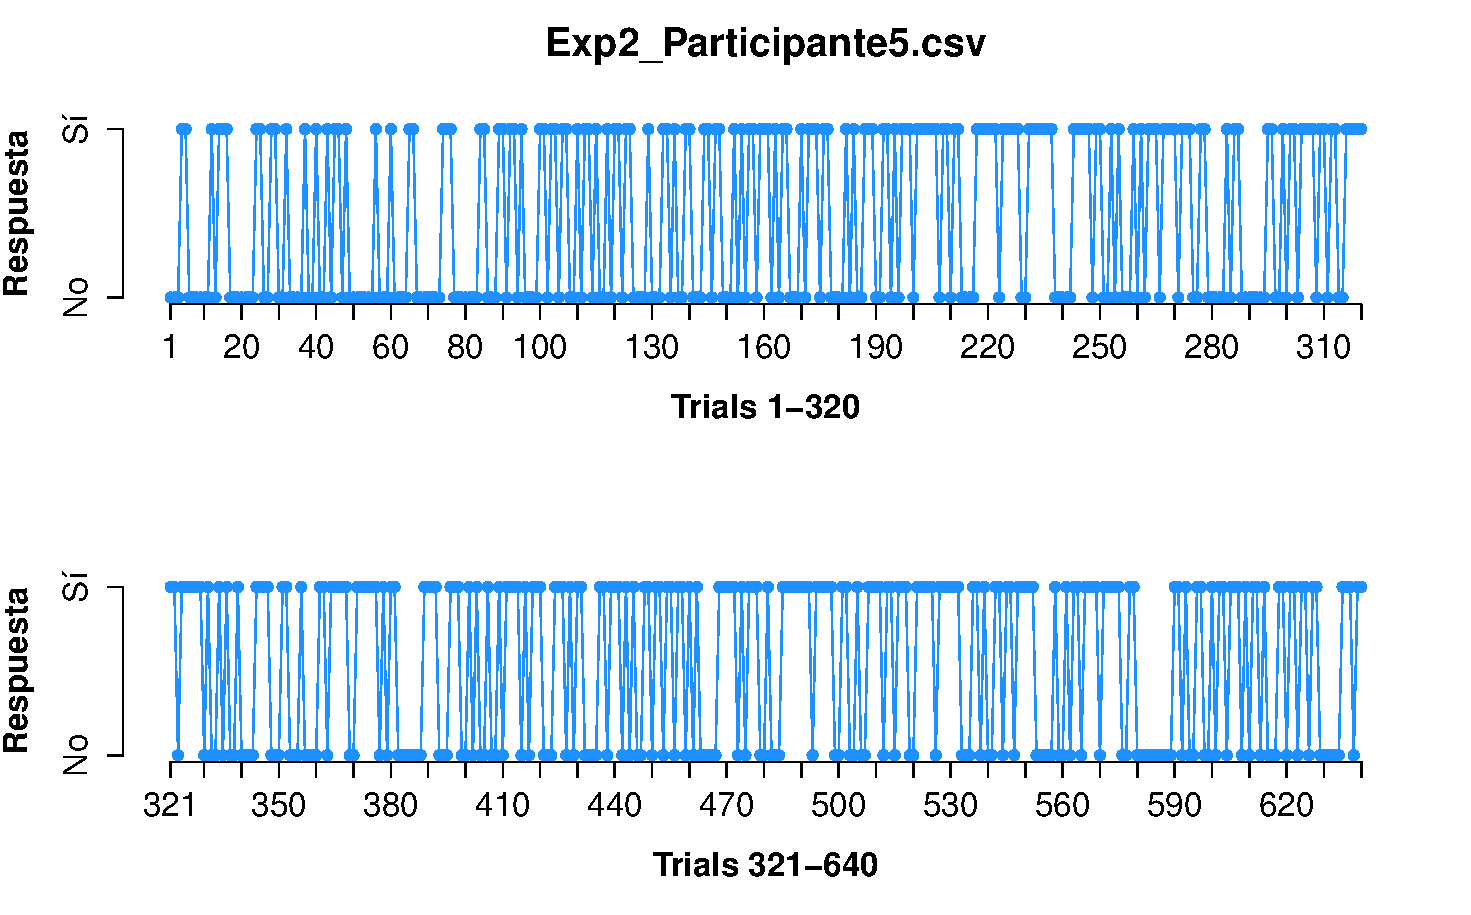
\includegraphics[width=0.30\textwidth]{Figures/Response_Exp2_P5} 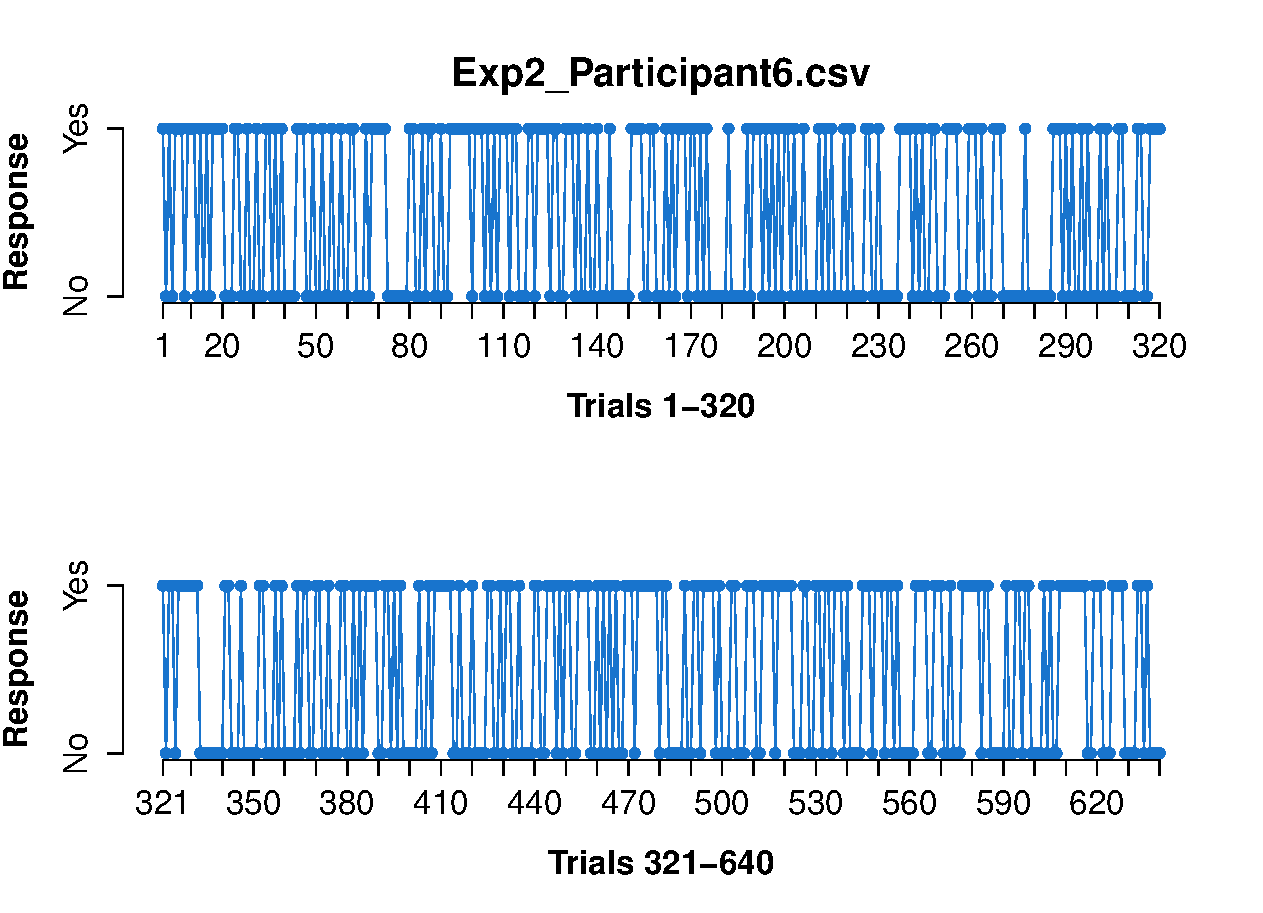
\includegraphics[width=0.30\textwidth]{Figures/Response_Exp2_P6}
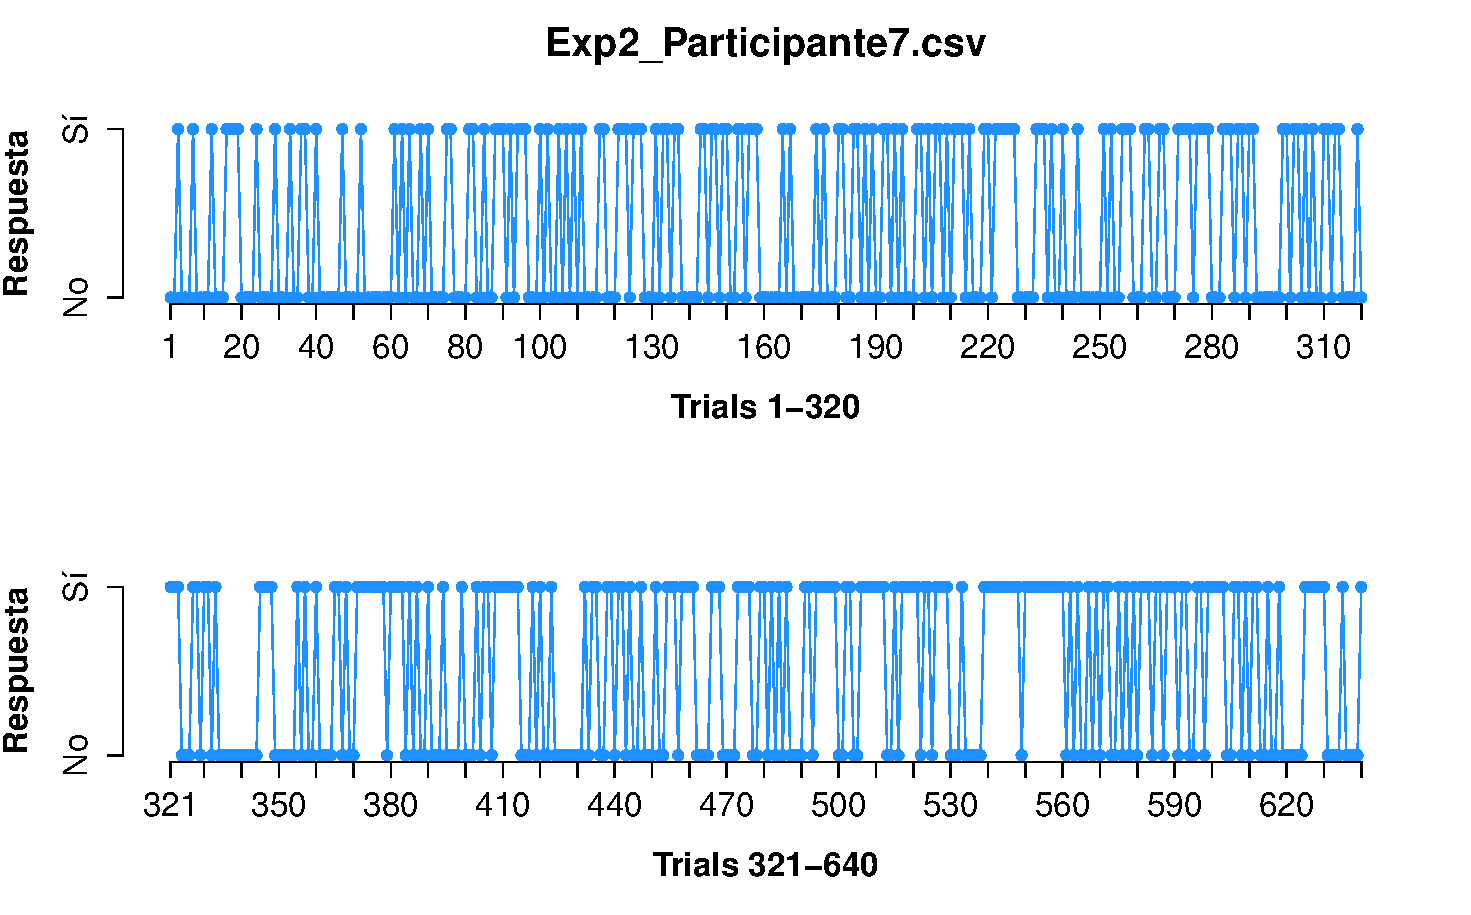
\includegraphics[width=0.30\textwidth]{Figures/Response_Exp2_P7} 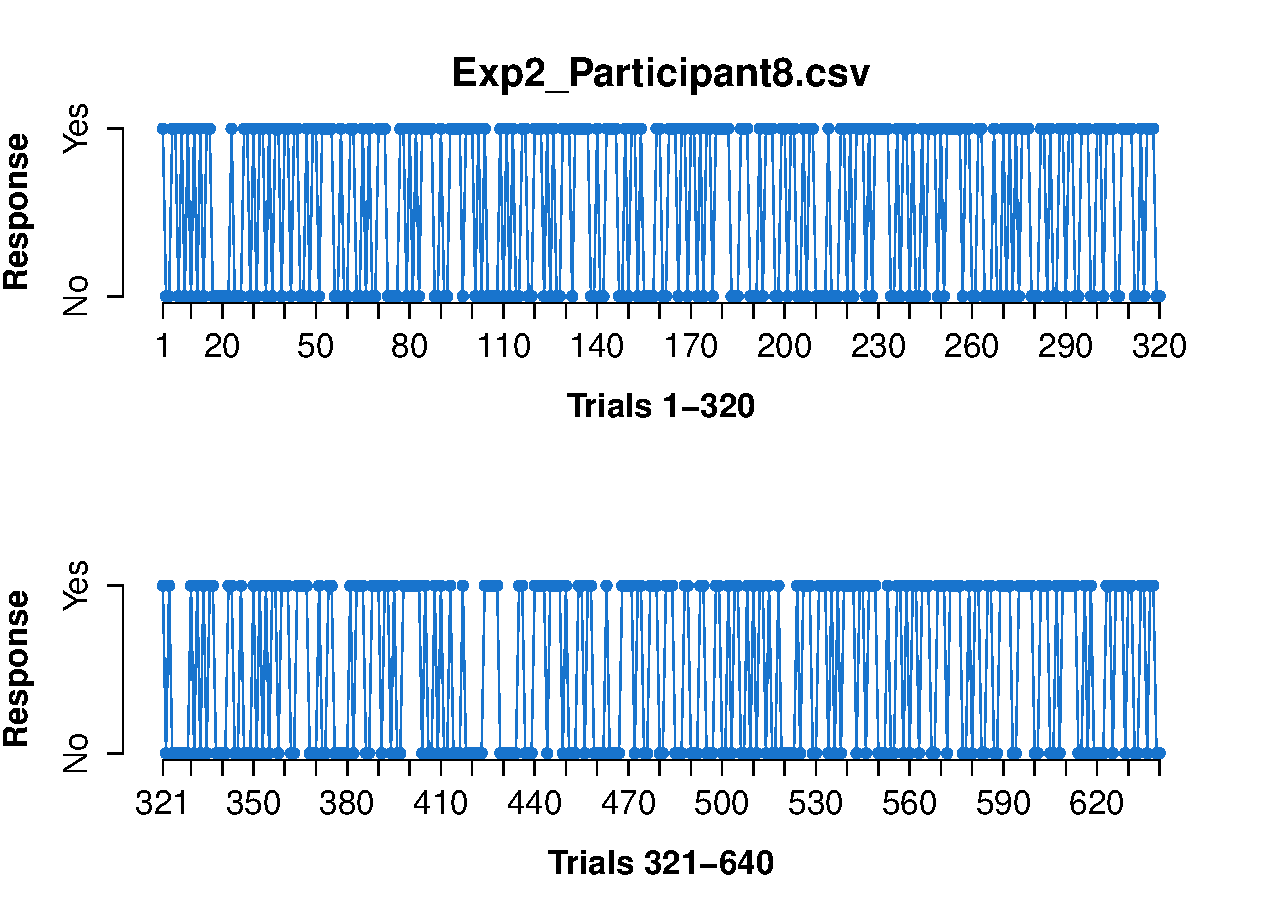
\includegraphics[width=0.30\textwidth]{Figures/Response_Exp2_P8} 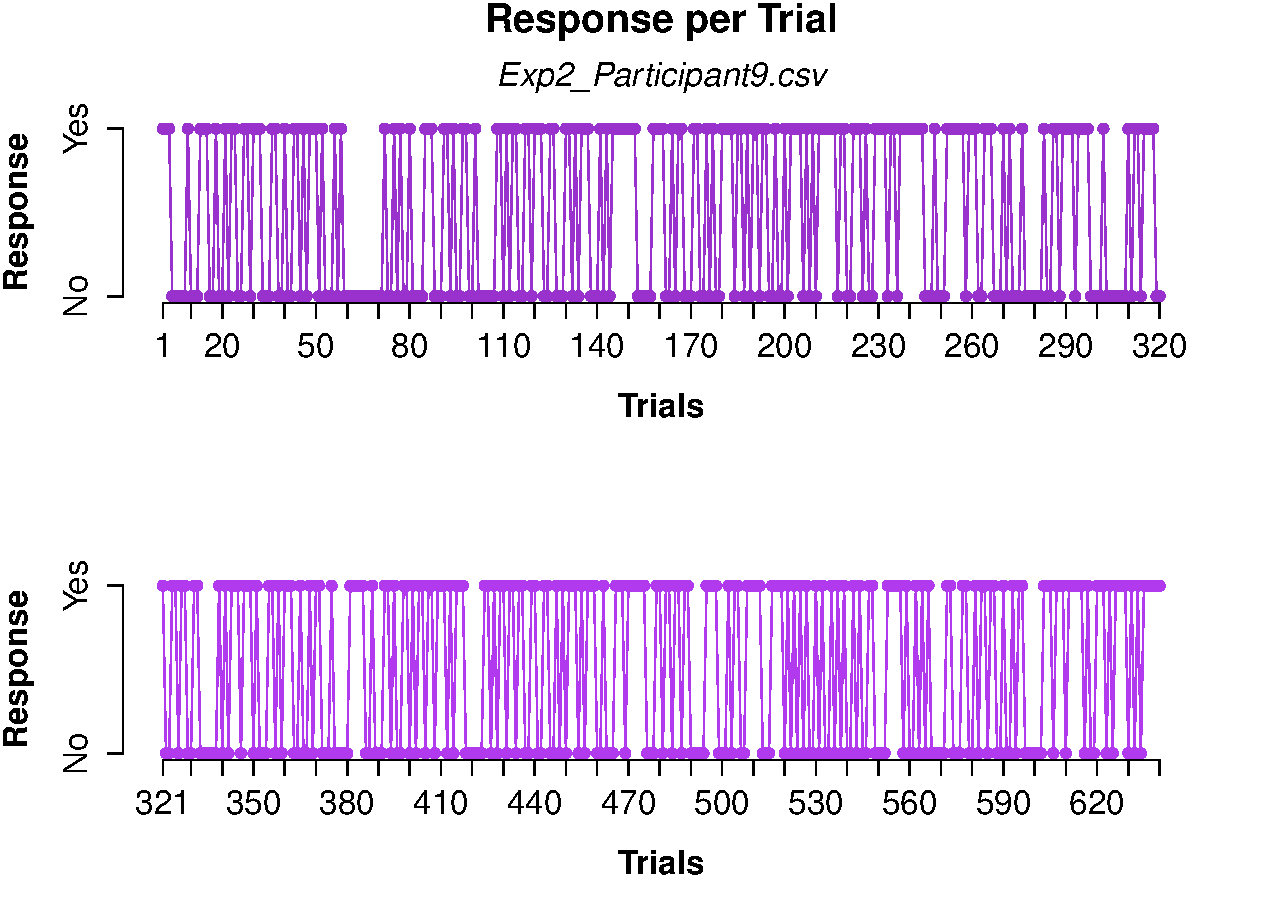
\includegraphics[width=0.30\textwidth]{Figures/Response_Exp2_P9}
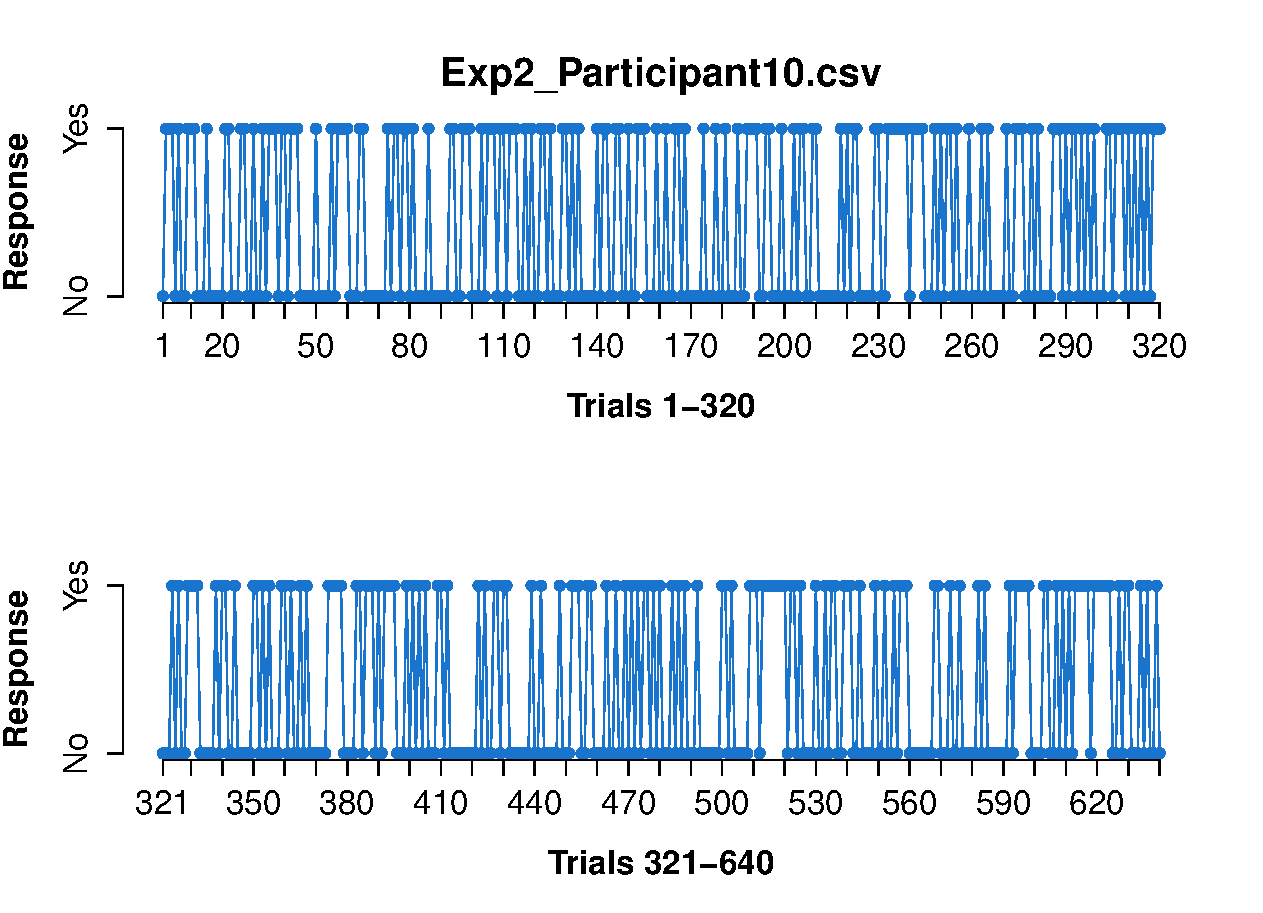
\includegraphics[width=0.30\textwidth]{Figures/Response_Exp2_P10} 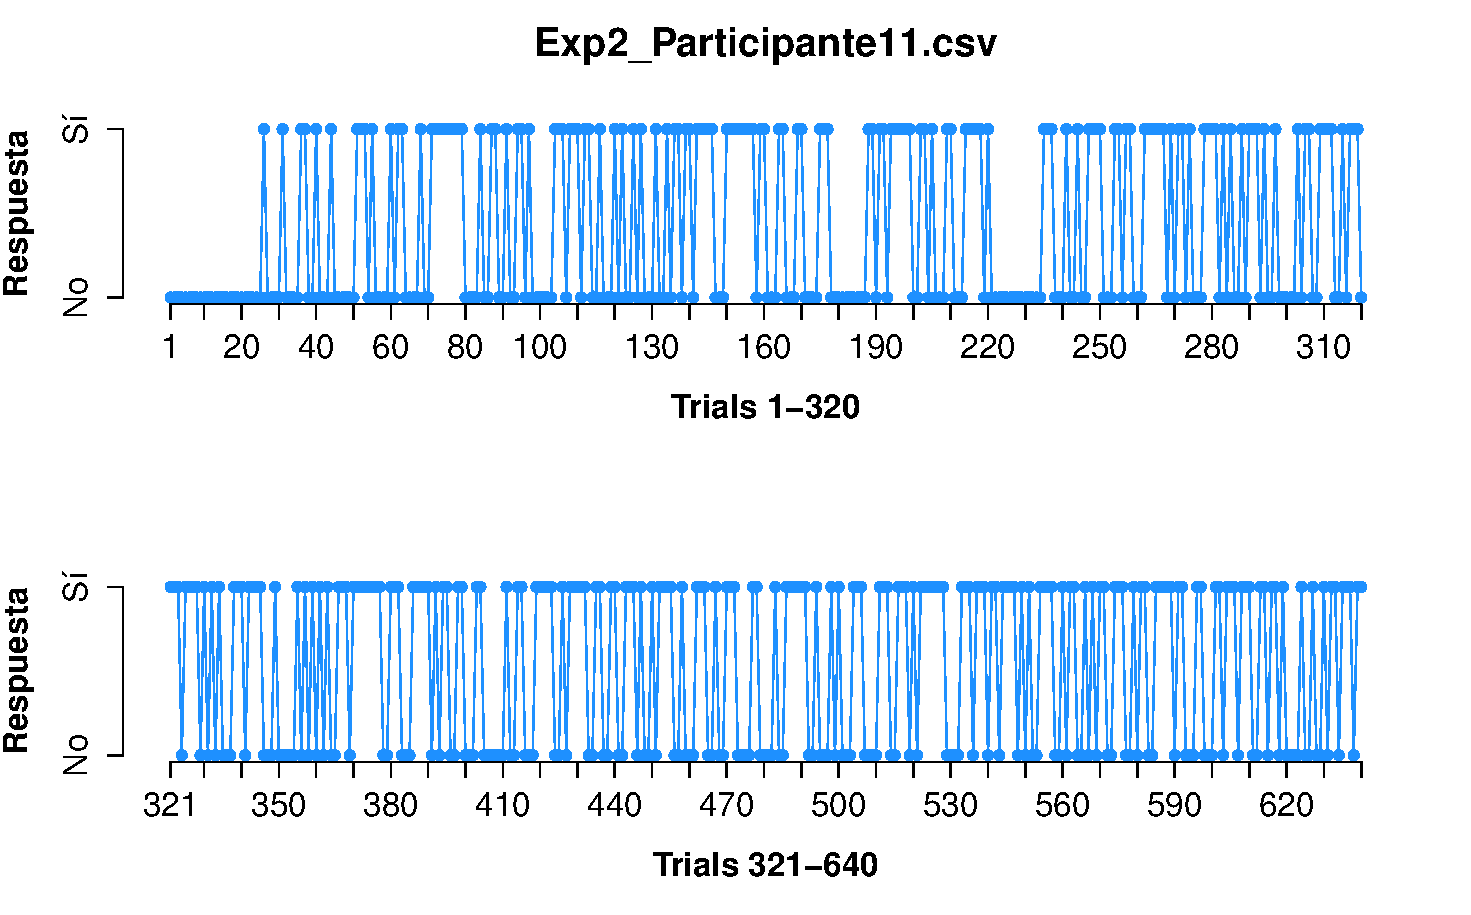
\includegraphics[width=0.30\textwidth]{Figures/Response_Exp2_P11} 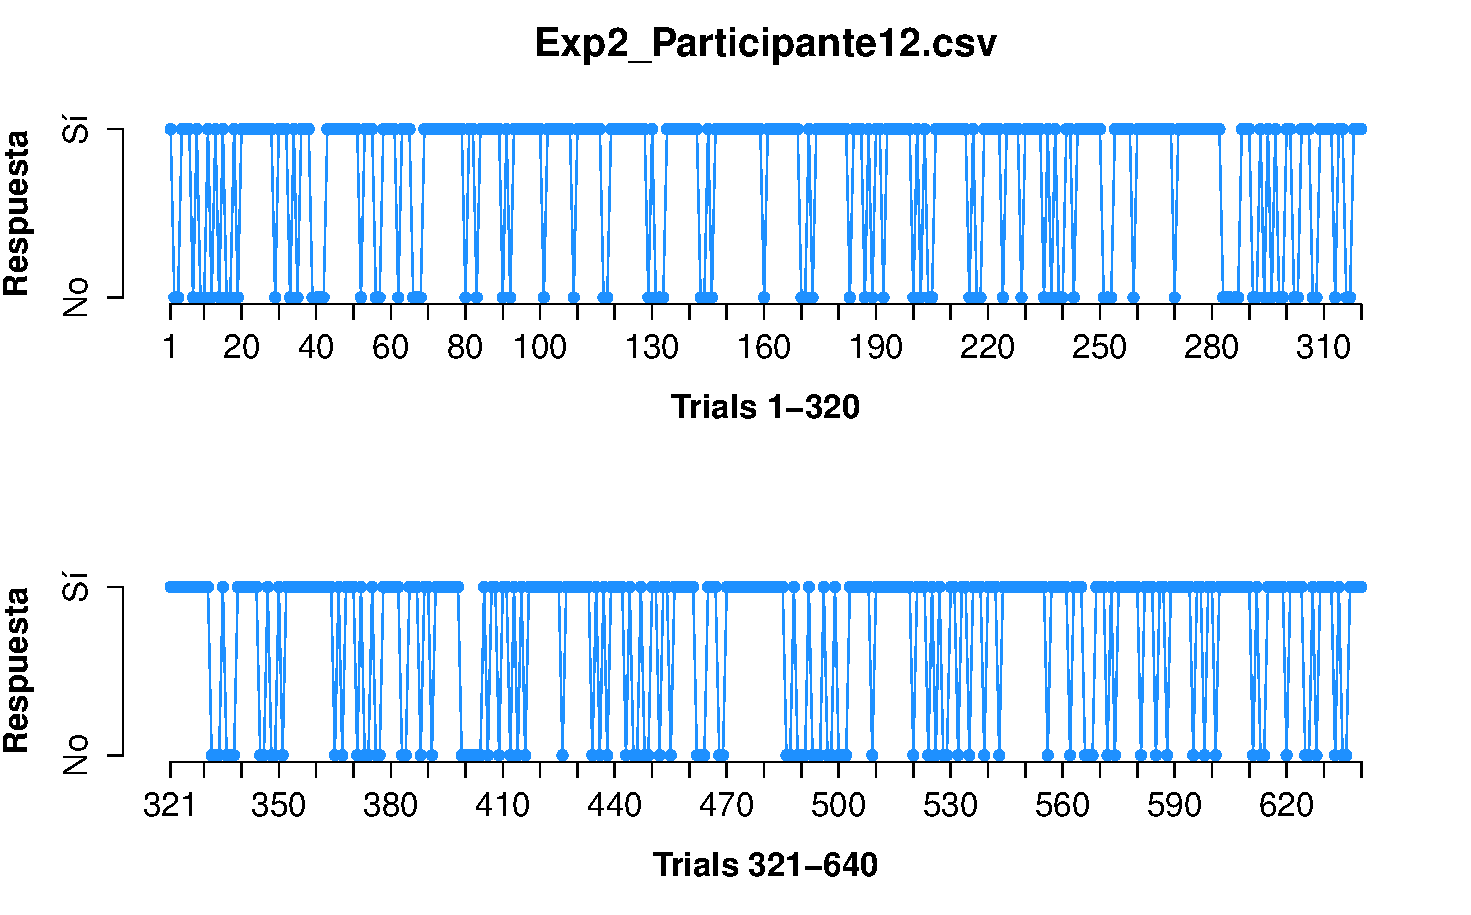
\includegraphics[width=0.30\textwidth]{Figures/Response_Exp2_P12}
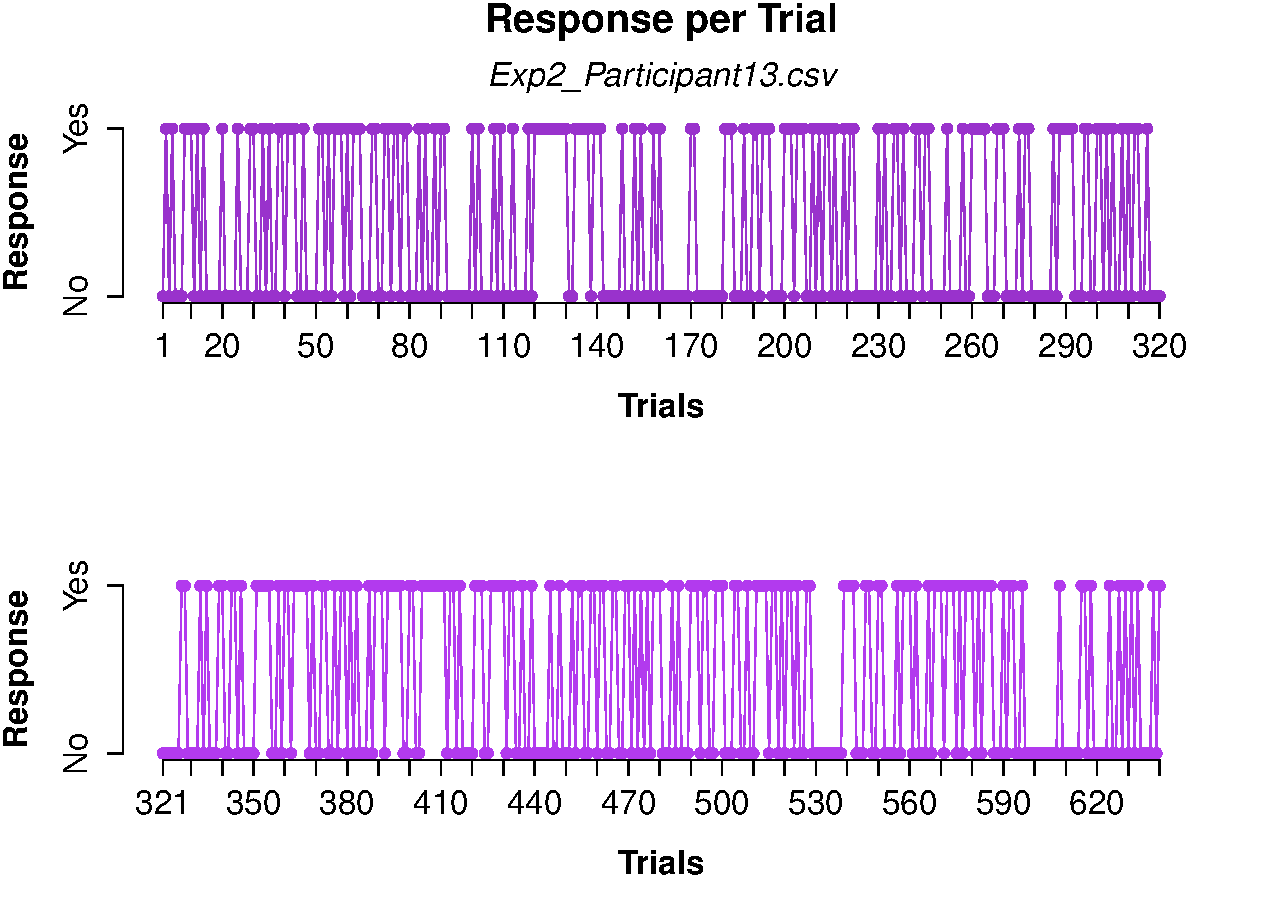
\includegraphics[width=0.30\textwidth]{Figures/Response_Exp2_P13} 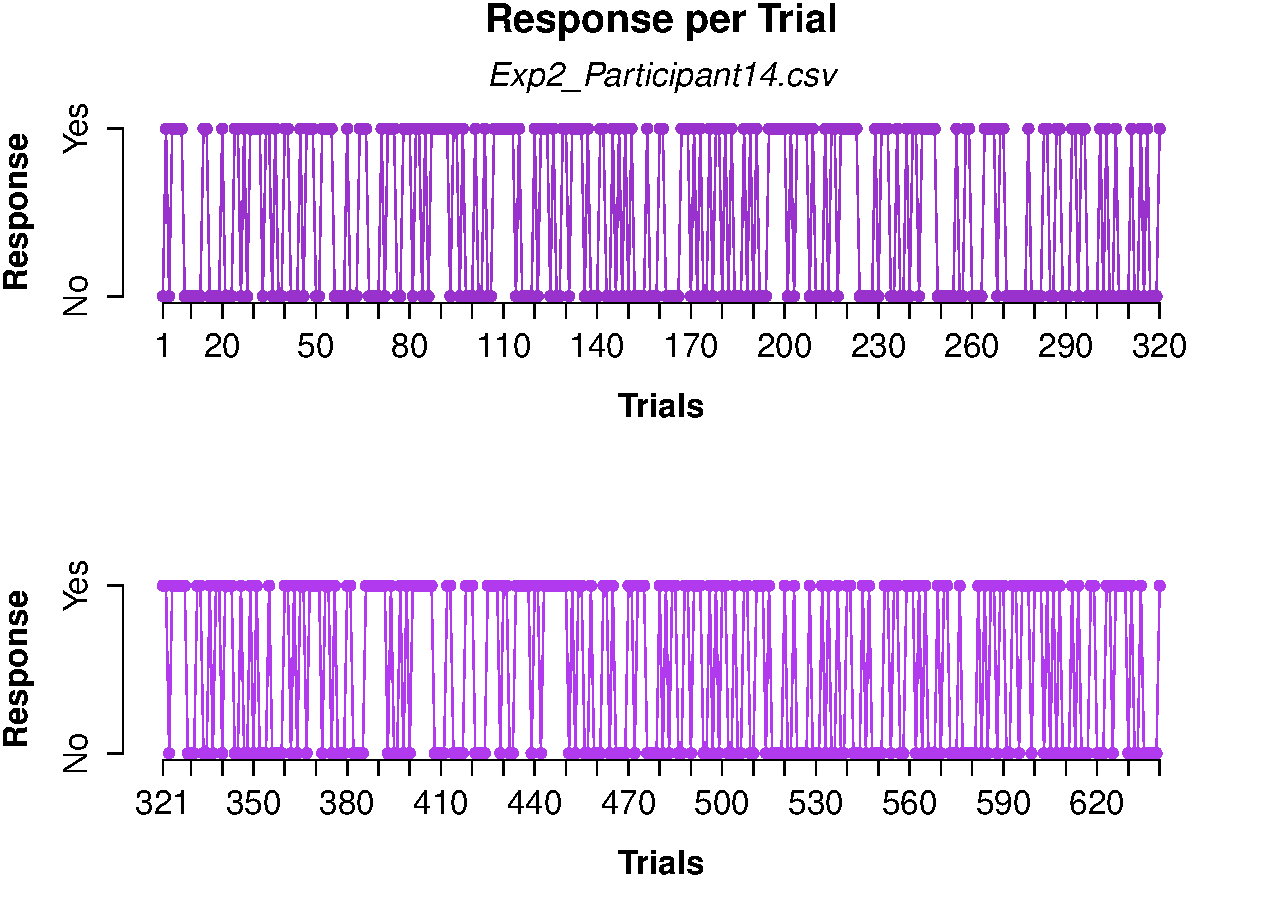
\includegraphics[width=0.30\textwidth]{Figures/Response_Exp2_P14} 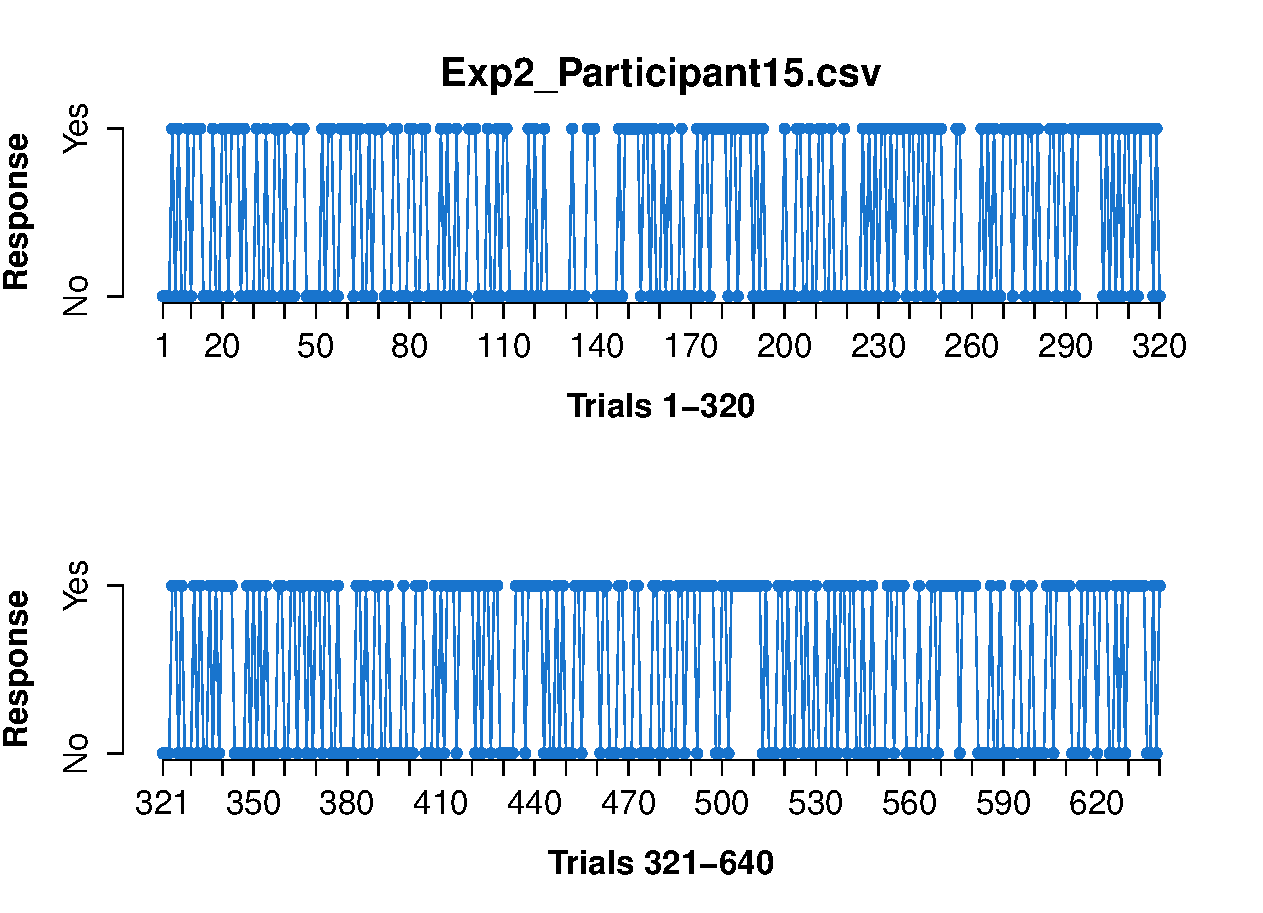
\includegraphics[width=0.30\textwidth]{Figures/Response_Exp2_P15}
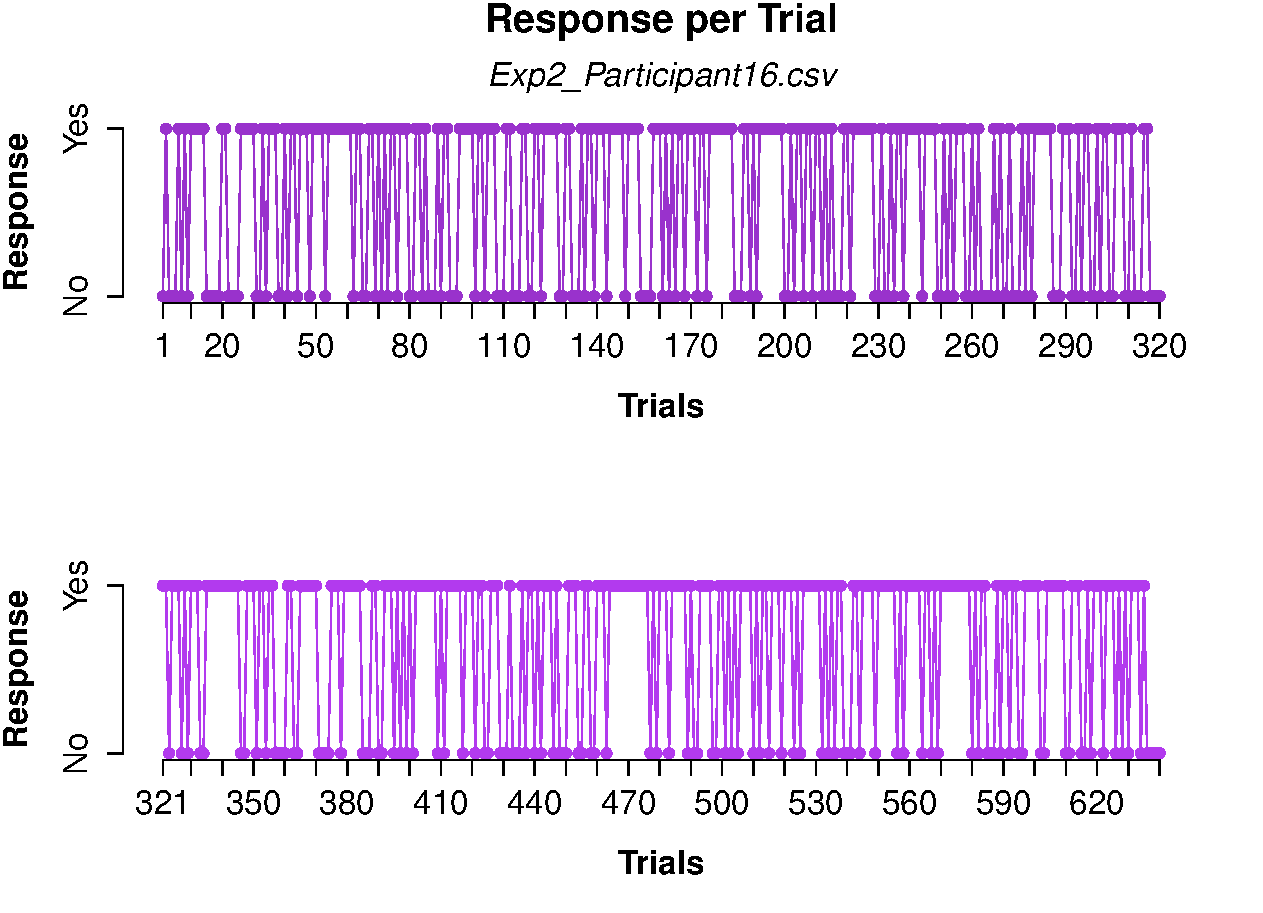
\includegraphics[width=0.30\textwidth]{Figures/Response_Exp2_P16} 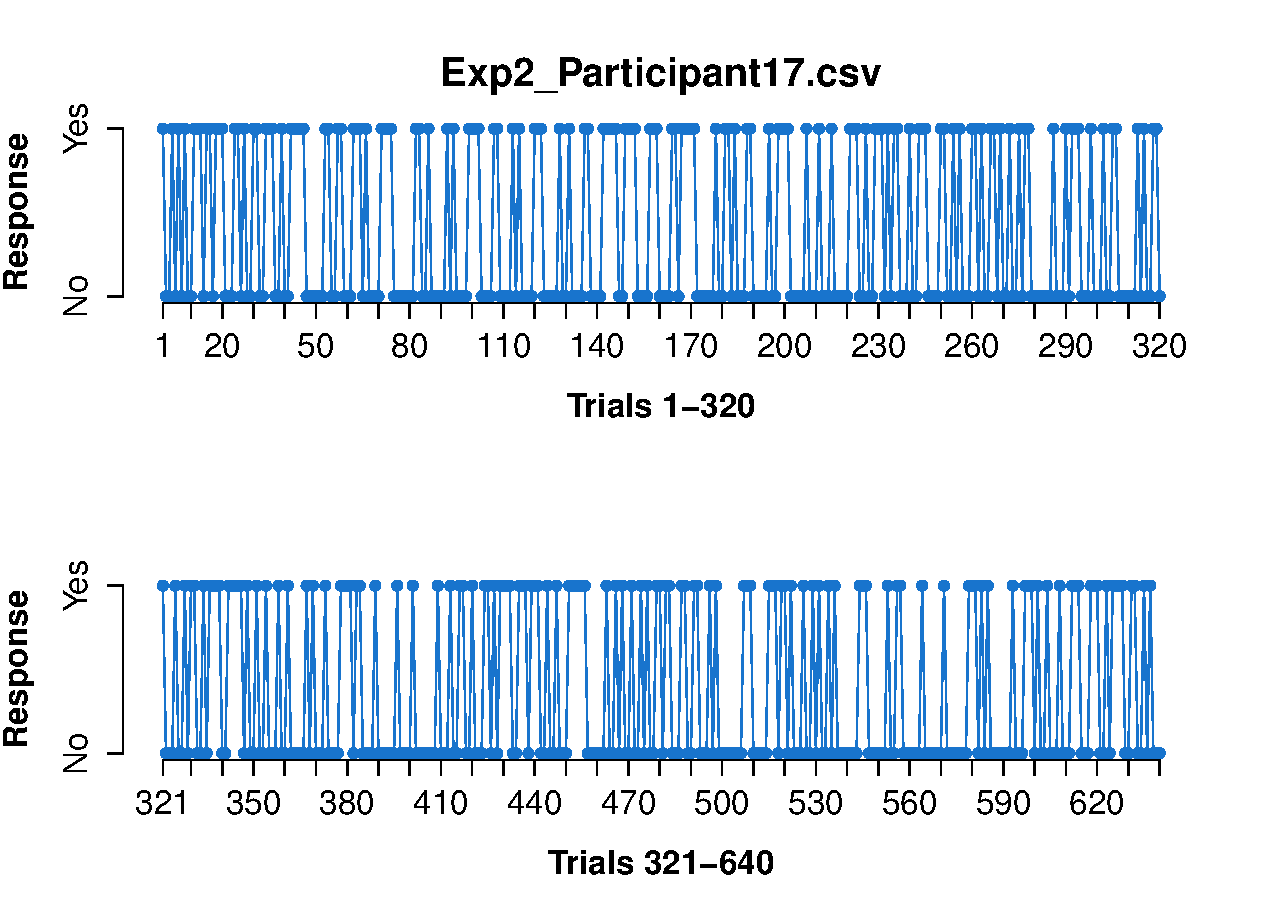
\includegraphics[width=0.30\textwidth]{Figures/Response_Exp2_P17} 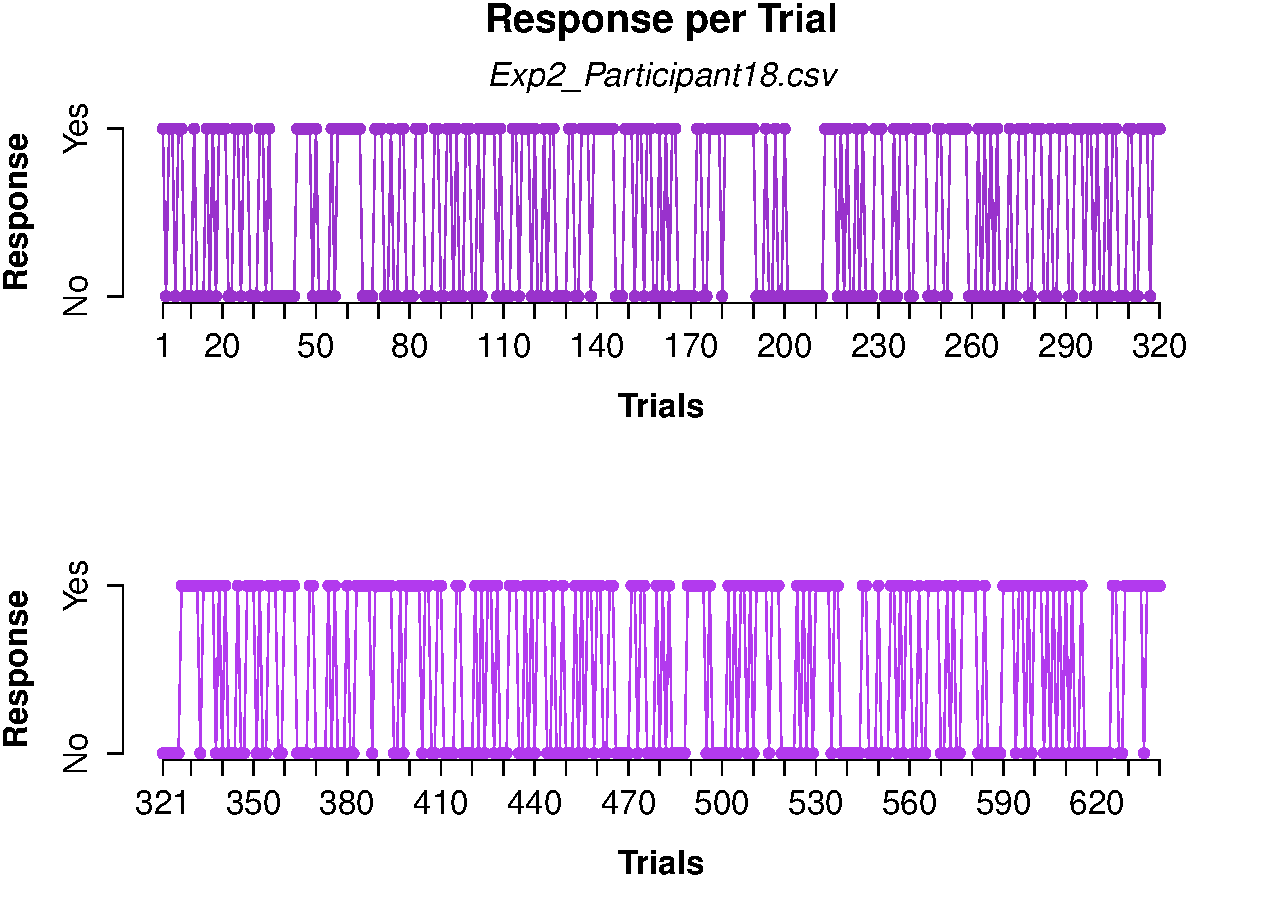
\includegraphics[width=0.30\textwidth]{Figures/Response_Exp2_P18}
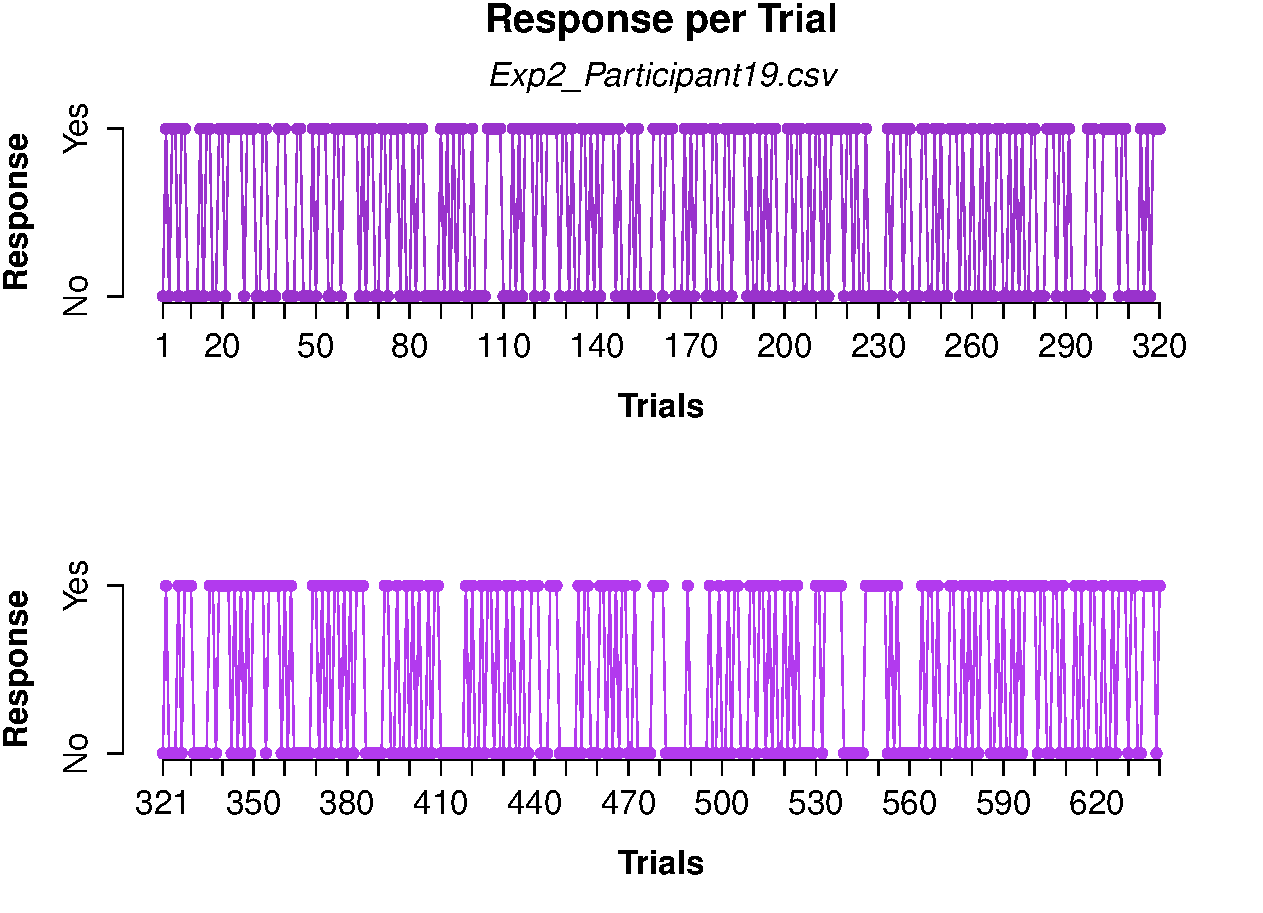
\includegraphics[width=0.30\textwidth]{Figures/Response_Exp2_P19} 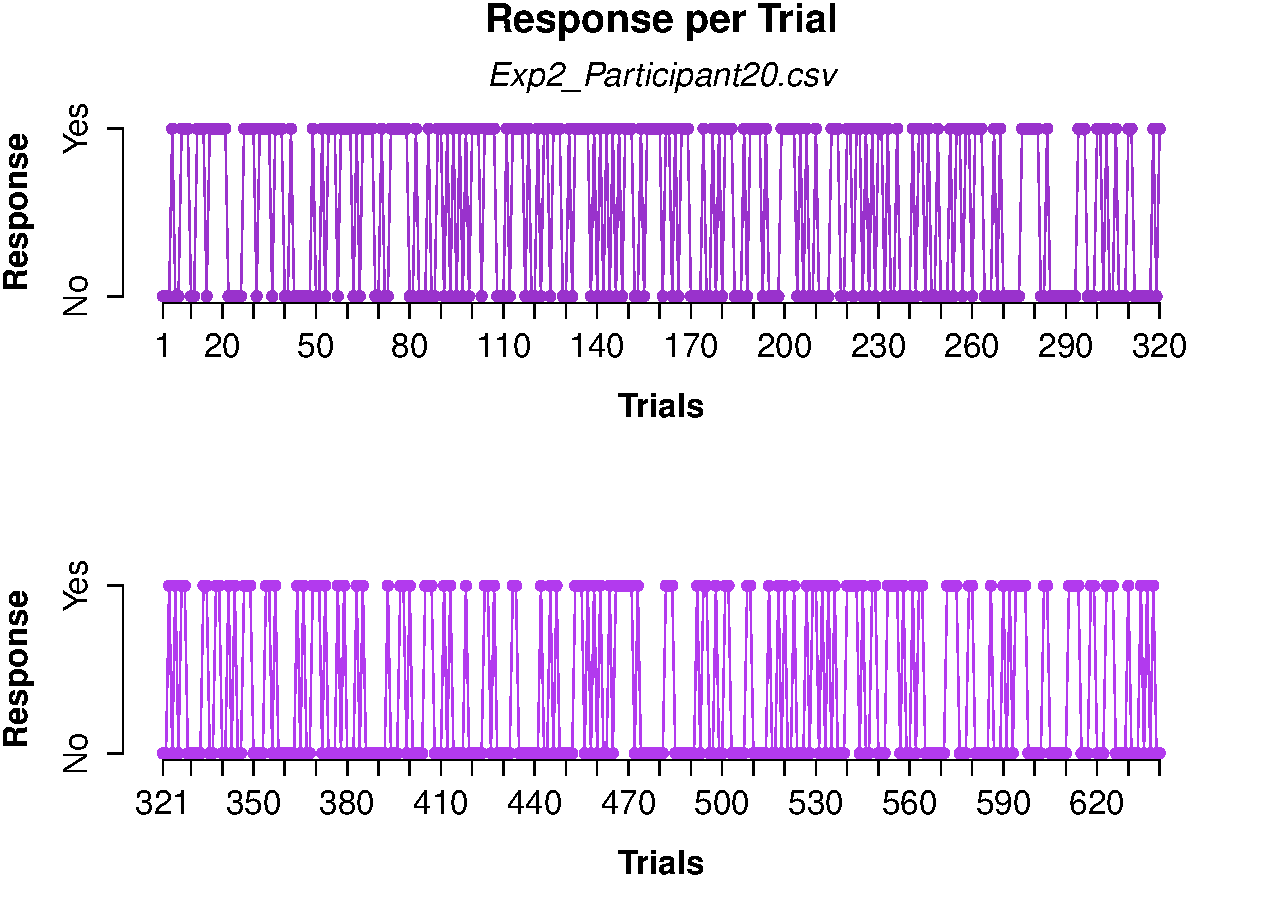
\includegraphics[width=0.30\textwidth]{Figures/Response_Exp2_P20} 
%\decoRule
\caption[Response_Exp2]{Respuesta registrada, ensayo a ensayo, durante la tarea de detección binaria por cada uno de los veinte participantes del Experimento 2. Las elecciones de cada participante se muestran a lo largo de dos gráficas que representan los primeros y los últimos 320 ensayos del experimento (panel superior e inferior, respectivamente).}
\label{fig:Response_E2}
\end{figure}

\begin{figure}[th]
\centering
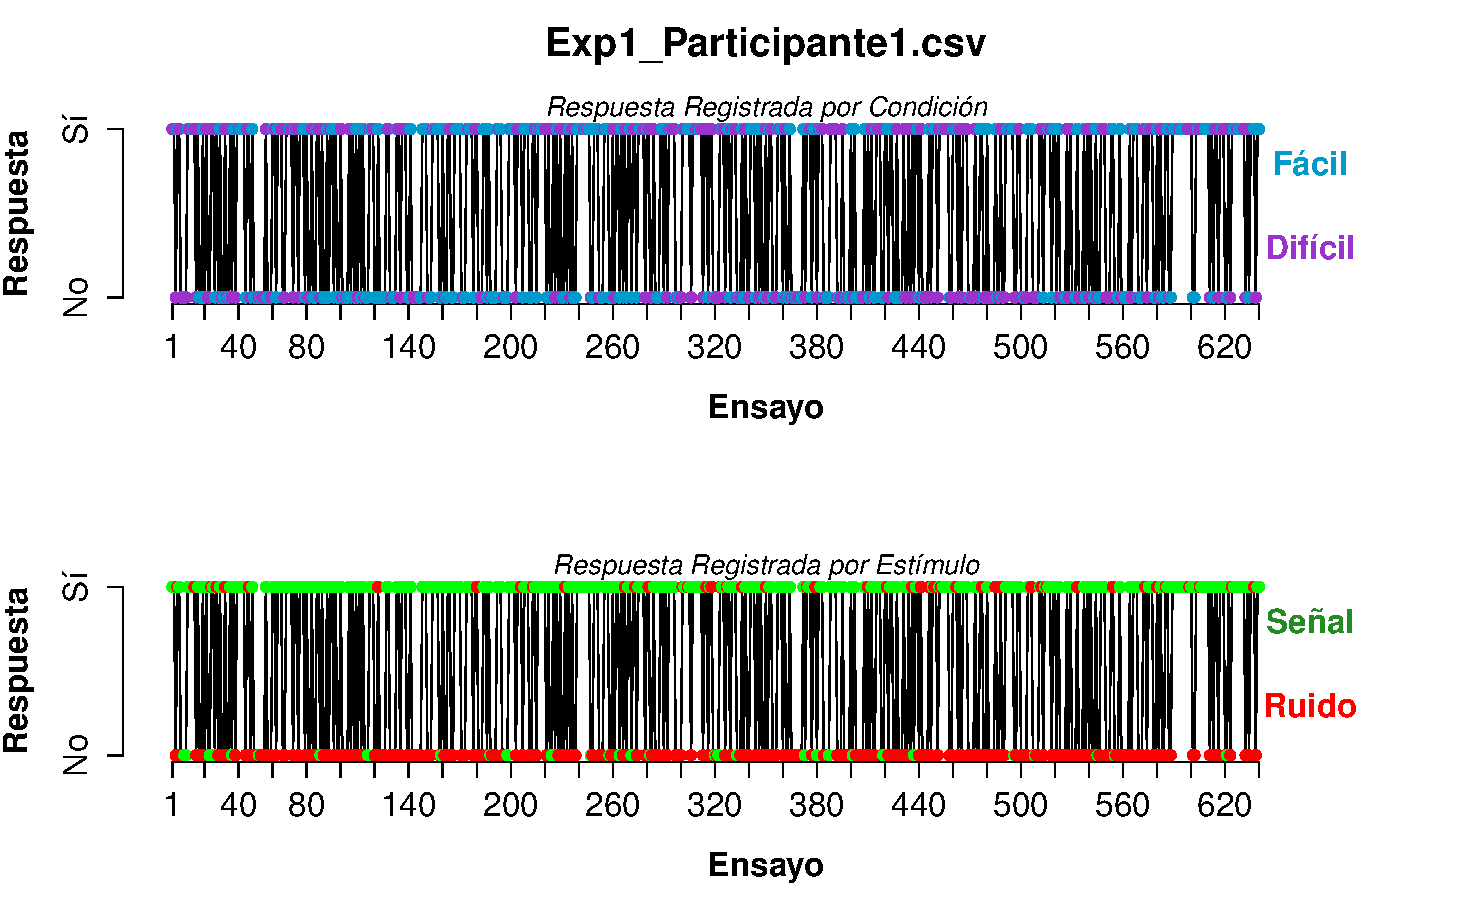
\includegraphics[width=0.30\textwidth]{Figures/BiasResp_Exp1_P1} 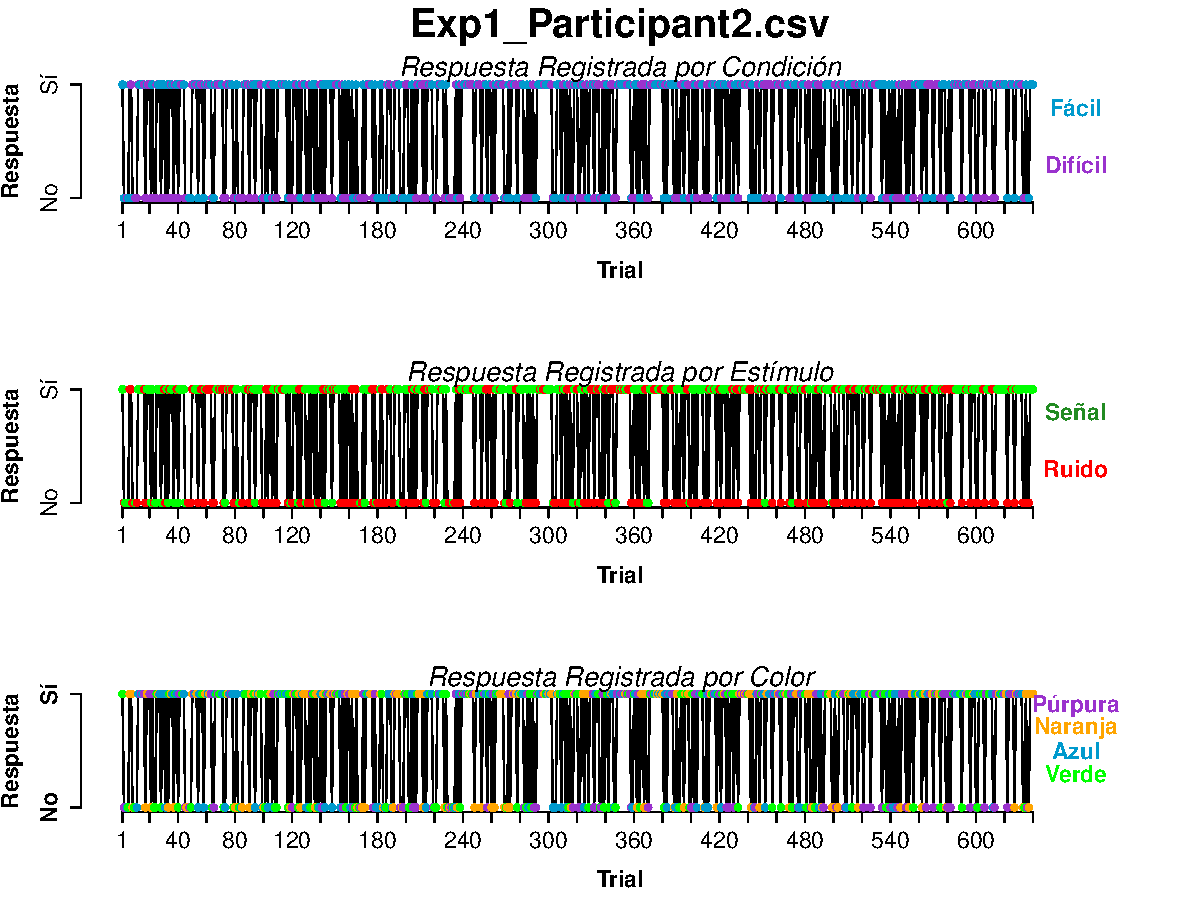
\includegraphics[width=0.30\textwidth]{Figures/BiasResp_Exp1_P2} 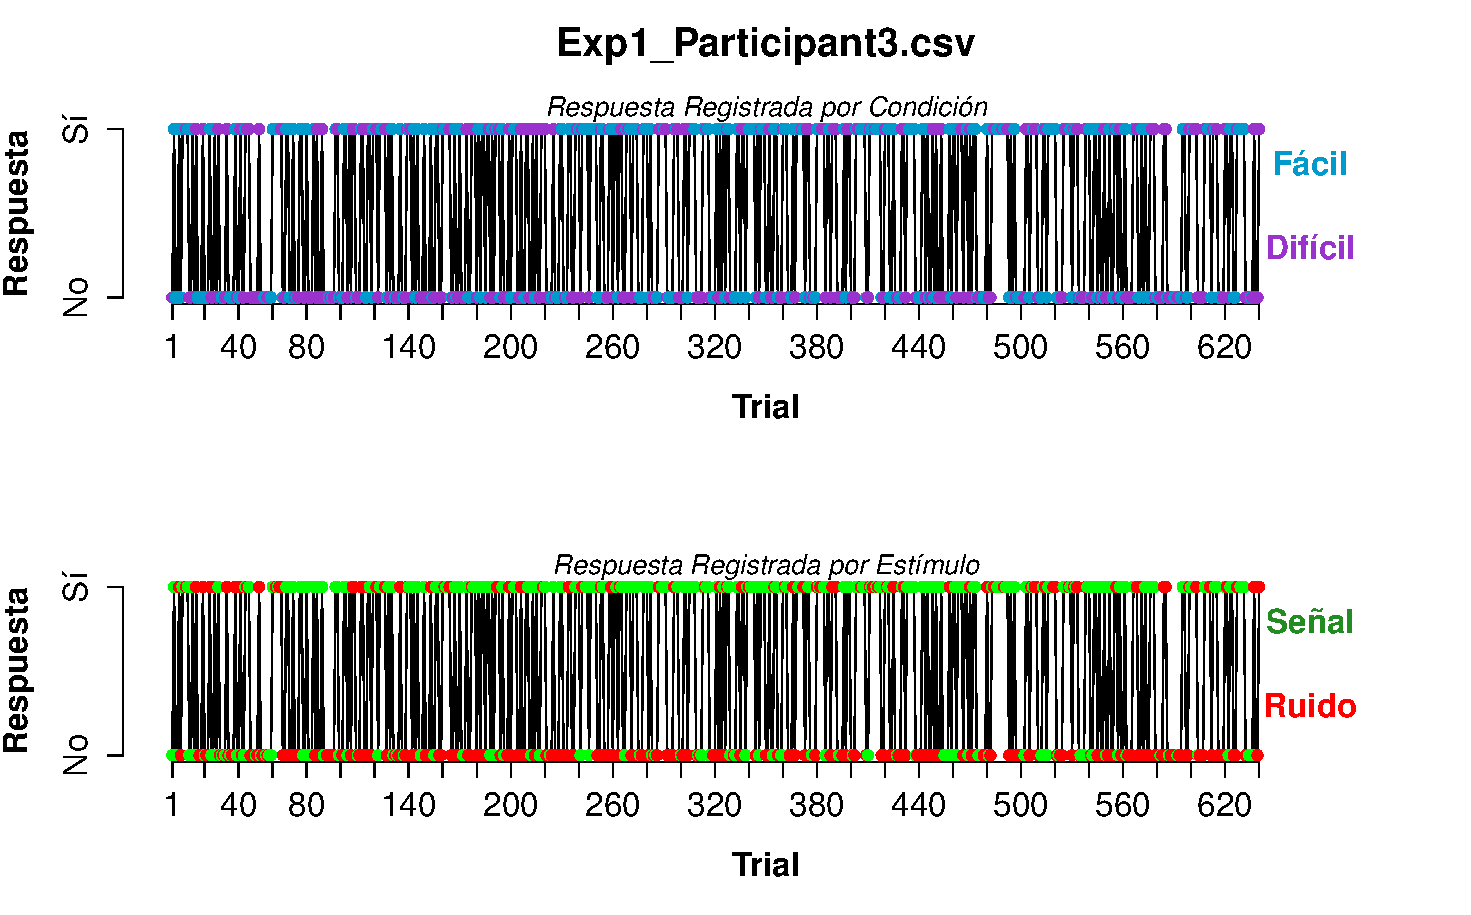
\includegraphics[width=0.30\textwidth]{Figures/BiasResp_Exp1_P3}
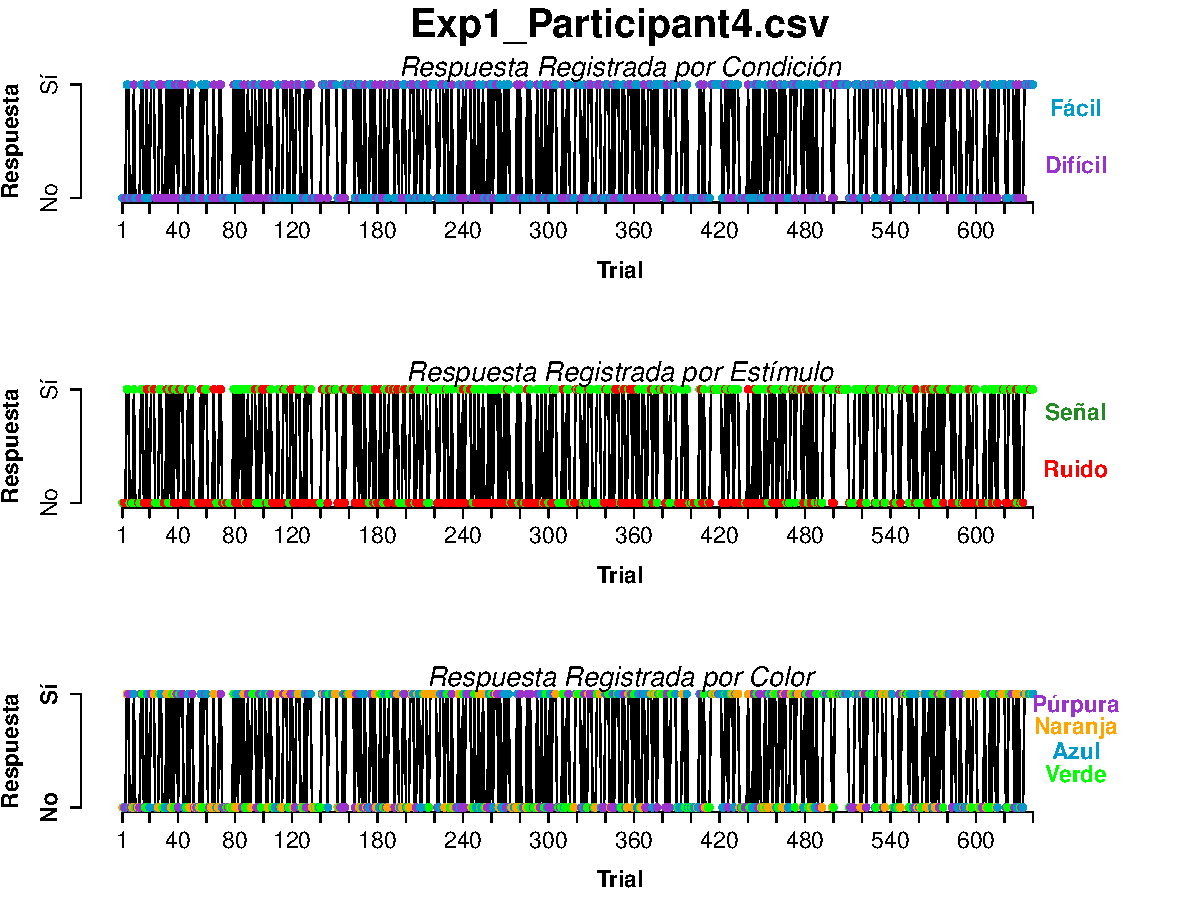
\includegraphics[width=0.30\textwidth]{Figures/BiasResp_Exp1_P4} 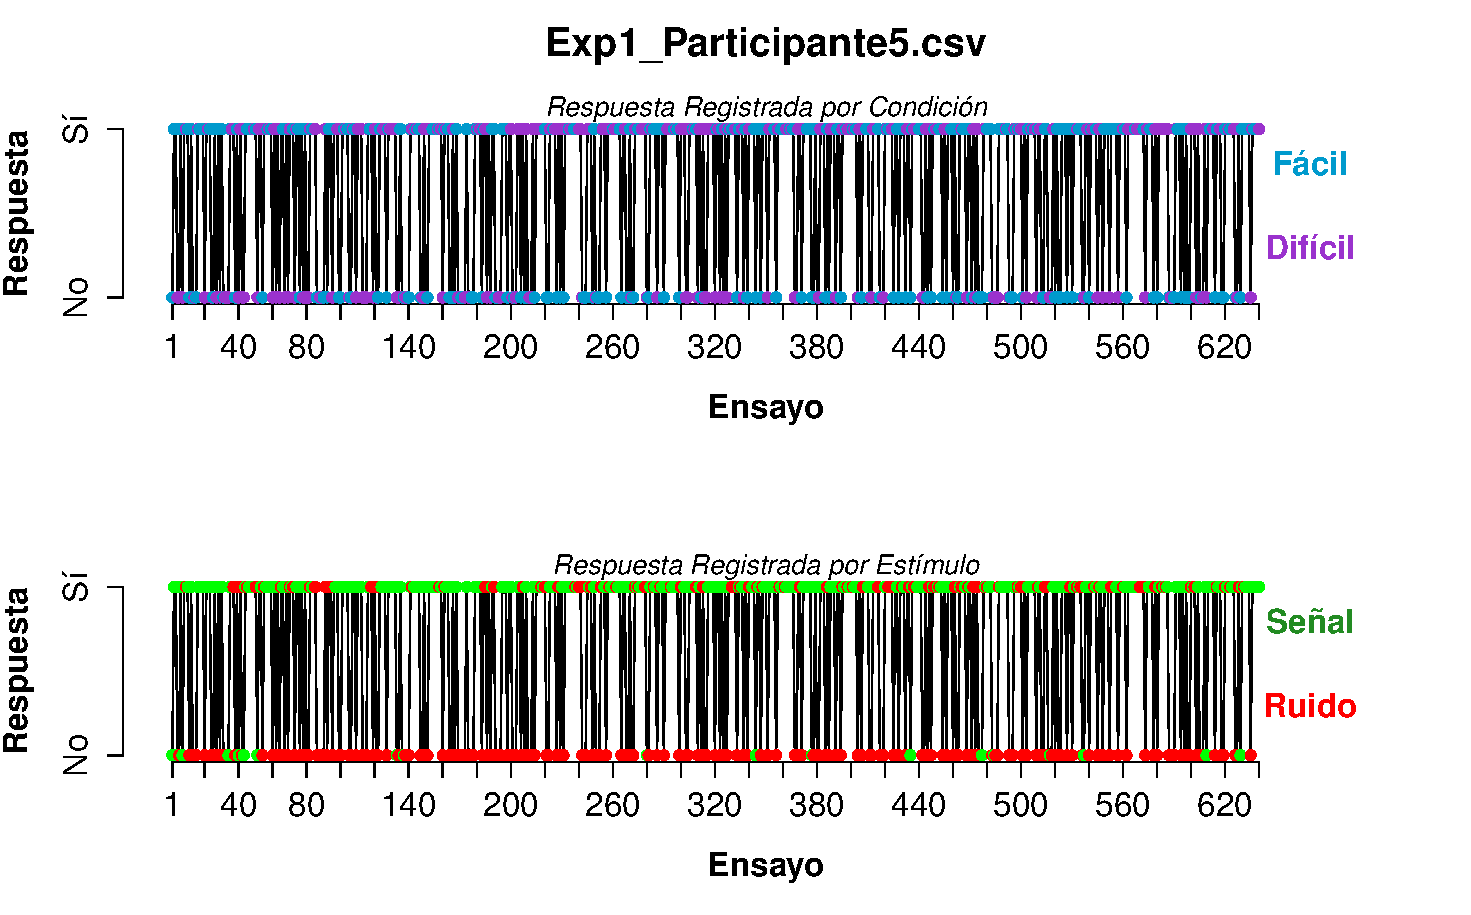
\includegraphics[width=0.30\textwidth]{Figures/BiasResp_Exp1_P5} 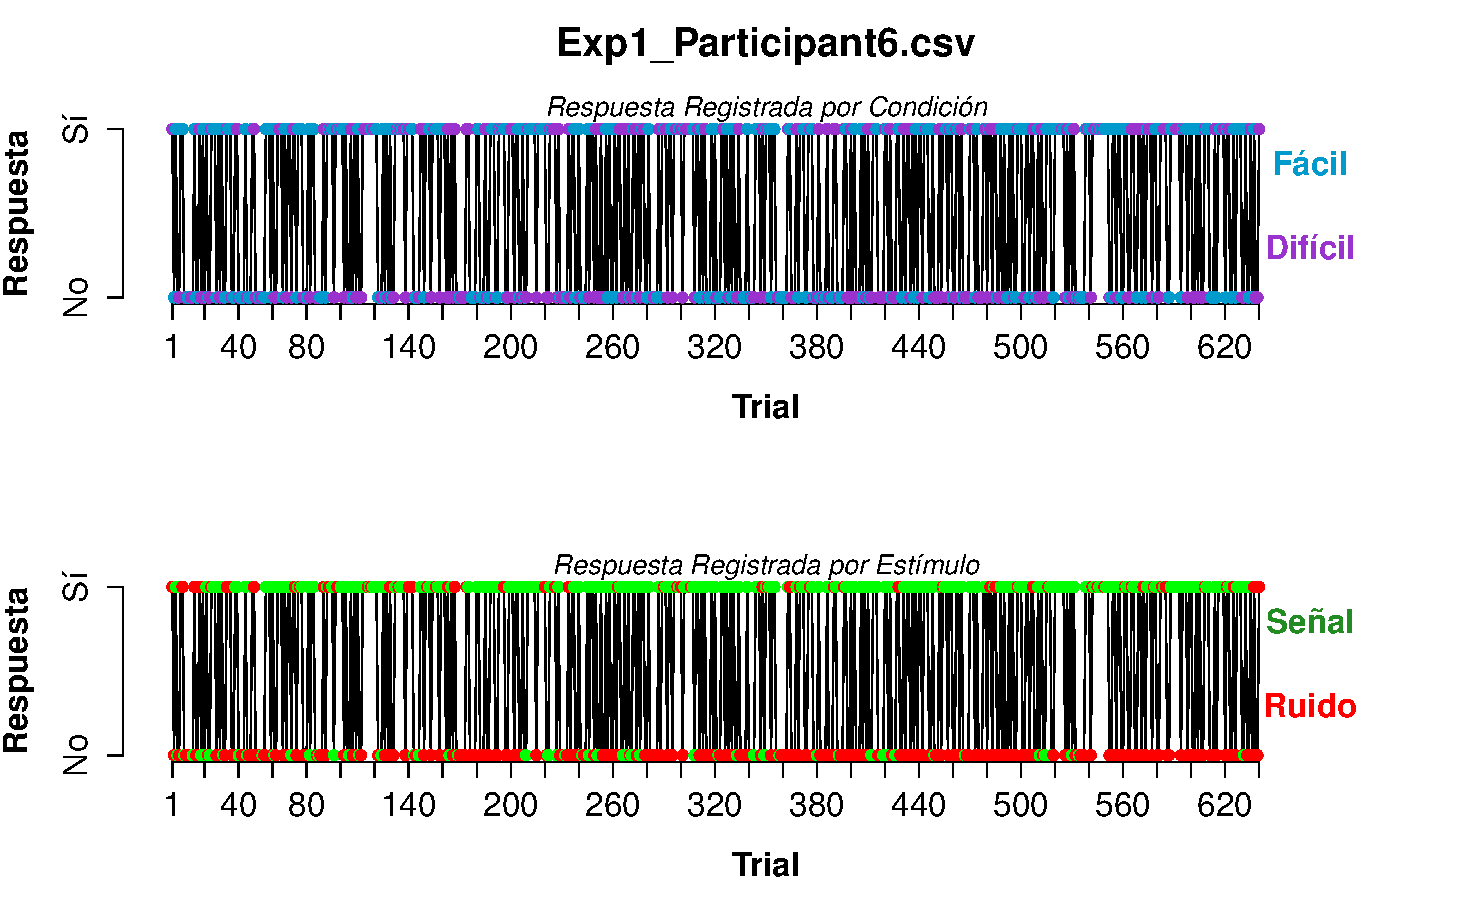
\includegraphics[width=0.30\textwidth]{Figures/BiasResp_Exp1_P6}
\includegraphics[width=0.30\textwidth]{Figures/BiasResp_Exp1_P7} \includegraphics[width=0.30\textwidth]{Figures/BiasResp_Exp1_P8} \includegraphics[width=0.30\textwidth]{Figures/BiasResp_Exp1_P9}
\includegraphics[width=0.30\textwidth]{Figures/BiasResp_Exp1_P10} \includegraphics[width=0.30\textwidth]{Figures/BiasResp_Exp1_P11} \includegraphics[width=0.30\textwidth]{Figures/BiasResp_Exp1_P12}
\includegraphics[width=0.30\textwidth]{Figures/BiasResp_Exp1_P13} \includegraphics[width=0.30\textwidth]{Figures/BiasResp_Exp1_P14} \includegraphics[width=0.30\textwidth]{Figures/BiasResp_Exp1_P15}
\includegraphics[width=0.30\textwidth]{Figures/BiasResp_Exp1_P16} \includegraphics[width=0.30\textwidth]{Figures/BiasResp_Exp1_P17} \includegraphics[width=0.30\textwidth]{Figures/BiasResp_Exp1_P18}
\includegraphics[width=0.30\textwidth]{Figures/BiasResp_Exp1_P19} \includegraphics[width=0.30\textwidth]{Figures/BiasResp_Exp1_P20} \includegraphics[width=0.30\textwidth]{Figures/BiasResp_Exp1_P21}
%\decoRule
\caption[ _Ex1]{Respuesta registrada por cada ensayo durante la tarea de detección binaria por cada uno de los veintiun participantes del Experimento 1. Por cada participante, se muestran tres gráficos distintos que relacionan la respuesta emitida en cada ensayo con la naturaleza del estímulo en cuestión; en el gráfico superior, se señalan con color púrpura los ensayos en que se mostró un estímulo difícil y en azul, los fáciles; en el panel intermedio se muestran en verde los estímulos donde los círculos a comparar eran del mismo tamaño (señal), y en rojo los ensayos en que esto no era el caso (ruido); el panel inferior muestra el color del estímulo en pantalla.}
\label{fig:BiasResp_E1}
\end{figure}

\begin{figure}[th]
\centering
\includegraphics[width=0.30\textwidth]{Figures/Rating_Exp2_P1} \includegraphics[width=0.30\textwidth]{Figures/Rating_Exp2_P2} \includegraphics[width=0.30\textwidth]{Figures/Rating_Exp2_P3}
\includegraphics[width=0.30\textwidth]{Figures/Rating_Exp2_P4} \includegraphics[width=0.30\textwidth]{Figures/Rating_Exp2_P5} \includegraphics[width=0.30\textwidth]{Figures/Rating_Exp2_P6}
\includegraphics[width=0.30\textwidth]{Figures/Rating_Exp2_P7} \includegraphics[width=0.30\textwidth]{Figures/Rating_Exp2_P8} \includegraphics[width=0.30\textwidth]{Figures/Rating_Exp2_P9}
\includegraphics[width=0.30\textwidth]{Figures/Rating_Exp2_P10} \includegraphics[width=0.30\textwidth]{Figures/Rating_Exp2_P11} \includegraphics[width=0.30\textwidth]{Figures/Rating_Exp2_P12}
\includegraphics[width=0.30\textwidth]{Figures/Rating_Exp2_P13} \includegraphics[width=0.30\textwidth]{Figures/Rating_Exp2_P14} \includegraphics[width=0.30\textwidth]{Figures/Rating_Exp2_P15}
\includegraphics[width=0.30\textwidth]{Figures/Rating_Exp2_P16} \includegraphics[width=0.30\textwidth]{Figures/Rating_Exp2_P17} \includegraphics[width=0.30\textwidth]{Figures/Rating_Exp2_P18}
\includegraphics[width=0.30\textwidth]{Figures/Rating_Exp2_P19} \includegraphics[width=0.30\textwidth]{Figures/Rating_Exp2_P20} 
%\decoRule
\caption[Rating_Exp2]{Puntaje asignado, ensayo a ensayo, a las respuestas emitidas durante la tarea de detección binaria por cada uno de los veinte participantes del Experimento 2. Las elecciones de cada participante se muestran en dos gráficos diferentes, donde se despliegan las respuestas dadas en la primer y segunda mitad del experimento (paneles superior e inferior, respectivamente). Durante el experimento, los participantes únicamente tuvieron que oprimir las teclas '1', '2' y '3', posteriormente el programa traducía estas respuestas en una escala mayor que distingue la certidumbre en la ausencia de la señal (i.e. '1' como 'muy seguro de que no') y la certidumbre de su presencia (i.e. '6' como 'muy seguro de que sí').}
\label{fig:Rating_E2}
\end{figure}
















\section{Control 2: Evaluando tiempos de respuesta a lo largo del experimento}

\begin{itemize}
\item Tiempos de Respuesta a 
\end{itemize}

\begin{figure}[th]
\centering
\includegraphics[width=0.30\textwidth]{Figures/RTs_Exp2_P1} \includegraphics[width=0.30\textwidth]{Figures/RTs_Exp2_P2} \includegraphics[width=0.30\textwidth]{Figures/RTs_Exp2_P3}
\includegraphics[width=0.30\textwidth]{Figures/RTs_Exp2_P4} \includegraphics[width=0.30\textwidth]{Figures/RTs_Exp2_P5} \includegraphics[width=0.30\textwidth]{Figures/RTs_Exp2_P6}
\includegraphics[width=0.30\textwidth]{Figures/RTs_Exp2_P7} \includegraphics[width=0.30\textwidth]{Figures/RTs_Exp2_P8} \includegraphics[width=0.30\textwidth]{Figures/RTs_Exp2_P9}
\includegraphics[width=0.30\textwidth]{Figures/RTs_Exp2_P10} \includegraphics[width=0.30\textwidth]{Figures/RTs_Exp2_P11} \includegraphics[width=0.30\textwidth]{Figures/RTs_Exp2_P12}
\includegraphics[width=0.30\textwidth]{Figures/RTs_Exp2_P13} \includegraphics[width=0.30\textwidth]{Figures/RTs_Exp2_P14} \includegraphics[width=0.30\textwidth]{Figures/RTs_Exp2_P15}
\includegraphics[width=0.30\textwidth]{Figures/RTs_Exp2_P16} \includegraphics[width=0.30\textwidth]{Figures/RTs_Exp2_P17} \includegraphics[width=0.30\textwidth]{Figures/RTs_Exp2_P18}
\includegraphics[width=0.30\textwidth]{Figures/RTs_Exp2_P19} \includegraphics[width=0.30\textwidth]{Figures/RTs_Exp2_P20} 
%\decoRule
\caption[TRs_Exp2]{Tiempos de Respuesta por ensayo (Experimento 2). Se muestran simultáneamente el tiempo de respuesta a la tarea principal (Color X) y a la escala de confianza (Color Y).}
\label{fig:RTs_E2}
\end{figure}

\begin{figure}[th]
\centering
\includegraphics[width=0.30\textwidth]{Figures/RT1_Exp2_P1} \includegraphics[width=0.30\textwidth]{Figures/RT1_Exp2_P2} \includegraphics[width=0.30\textwidth]{Figures/RT1_Exp2_P3}
\includegraphics[width=0.30\textwidth]{Figures/RT1_Exp2_P4} \includegraphics[width=0.30\textwidth]{Figures/RT1_Exp2_P5} \includegraphics[width=0.30\textwidth]{Figures/RT1_Exp2_P6}
\includegraphics[width=0.30\textwidth]{Figures/RT1_Exp2_P7} \includegraphics[width=0.30\textwidth]{Figures/RT1_Exp2_P8} \includegraphics[width=0.30\textwidth]{Figures/RT1_Exp2_P9}
\includegraphics[width=0.30\textwidth]{Figures/RT1_Exp2_P10} \includegraphics[width=0.30\textwidth]{Figures/RT1_Exp2_P11} \includegraphics[width=0.30\textwidth]{Figures/RT1_Exp2_P12}
\includegraphics[width=0.30\textwidth]{Figures/RT1_Exp2_P13} \includegraphics[width=0.30\textwidth]{Figures/RT1_Exp2_P14} \includegraphics[width=0.30\textwidth]{Figures/RT1_Exp2_P15}
\includegraphics[width=0.30\textwidth]{Figures/RT1_Exp2_P16} \includegraphics[width=0.30\textwidth]{Figures/RT1_Exp2_P17} \includegraphics[width=0.30\textwidth]{Figures/RT1_Exp2_P18}
\includegraphics[width=0.30\textwidth]{Figures/RT1_Exp2_P19} \includegraphics[width=0.30\textwidth]{Figures/RT1_Exp2_P20} 
%\decoRule
\caption[TR1_Exp2]{Tiempo de Respuesta a la tarea perceptual por ensayo (Experimento 2).}
\label{fig:RT1_E2}
\end{figure}

\begin{figure}[th]
\centering
\includegraphics[width=0.30\textwidth]{Figures/RT2_Exp2_P1} \includegraphics[width=0.30\textwidth]{Figures/RT2_Exp2_P2} \includegraphics[width=0.30\textwidth]{Figures/RT2_Exp2_P3}
\includegraphics[width=0.30\textwidth]{Figures/RT2_Exp2_P4} \includegraphics[width=0.30\textwidth]{Figures/RT2_Exp2_P5} \includegraphics[width=0.30\textwidth]{Figures/RT2_Exp2_P6}
\includegraphics[width=0.30\textwidth]{Figures/RT2_Exp2_P7} \includegraphics[width=0.30\textwidth]{Figures/RT2_Exp2_P8} \includegraphics[width=0.30\textwidth]{Figures/RT2_Exp2_P9}
\includegraphics[width=0.30\textwidth]{Figures/RT2_Exp2_P10} \includegraphics[width=0.30\textwidth]{Figures/RT2_Exp2_P11} \includegraphics[width=0.30\textwidth]{Figures/RT2_Exp2_P12}
\includegraphics[width=0.30\textwidth]{Figures/RT2_Exp2_P13} \includegraphics[width=0.30\textwidth]{Figures/RT2_Exp2_P14} \includegraphics[width=0.30\textwidth]{Figures/RT2_Exp2_P15}
\includegraphics[width=0.30\textwidth]{Figures/RT2_Exp2_P16} \includegraphics[width=0.30\textwidth]{Figures/RT2_Exp2_P17} \includegraphics[width=0.30\textwidth]{Figures/RT2_Exp2_P18}
\includegraphics[width=0.30\textwidth]{Figures/RT2_Exp2_P19} \includegraphics[width=0.30\textwidth]{Figures/RT2_Exp2_P20} 
%\decoRule
\caption[TR2_Exp2]{Tiempo de respuesta a la escala de confianza por ensayo (Experimento 2).}
\label{fig:RT2_E2}
\end{figure}
















\section{Control 3: ¿La duración del experimento tuvo un impacto en la ejecución de los participantes?}

\begin{itemize}
\item
\item
\end{itemize}

\begin{figure}[th]
\centering
\includegraphics[width=0.30\textwidth]{Figures/Success_Exp1_P1} \includegraphics[width=0.30\textwidth]{Figures/Success_Exp1_P2} \includegraphics[width=0.30\textwidth]{Figures/Success_Exp1_P3}
\includegraphics[width=0.30\textwidth]{Figures/Success_Exp1_P4} \includegraphics[width=0.30\textwidth]{Figures/Success_Exp1_P5} \includegraphics[width=0.30\textwidth]{Figures/Success_Exp1_P6}
\includegraphics[width=0.30\textwidth]{Figures/Success_Exp1_P7} \includegraphics[width=0.30\textwidth]{Figures/Success_Exp1_P8} \includegraphics[width=0.30\textwidth]{Figures/Success_Exp1_P9}
\includegraphics[width=0.30\textwidth]{Figures/Success_Exp1_P10} \includegraphics[width=0.30\textwidth]{Figures/Success_Exp1_P11} \includegraphics[width=0.30\textwidth]{Figures/Success_Exp1_P12}
\includegraphics[width=0.30\textwidth]{Figures/Success_Exp1_P13} \includegraphics[width=0.30\textwidth]{Figures/Success_Exp1_P14} \includegraphics[width=0.30\textwidth]{Figures/Success_Exp1_P15}
\includegraphics[width=0.30\textwidth]{Figures/Success_Exp1_P16} \includegraphics[width=0.30\textwidth]{Figures/Success_Exp1_P17} \includegraphics[width=0.30\textwidth]{Figures/Success_Exp1_P18}
\includegraphics[width=0.30\textwidth]{Figures/Success_Exp1_P19} \includegraphics[width=0.30\textwidth]{Figures/Success_Exp1_P20} \includegraphics[width=0.30\textwidth]{Figures/Success_Exp1_P21} 
%\decoRule
\caption[Success_Exp1]{Desempeño del participante a lo largo del experimento (Experimento 1).}
\label{fig:Success_E1}
\end{figure}

\begin{figure}[th]
\centering
\includegraphics[width=0.30\textwidth]{Figures/Success_Exp2_P1} \includegraphics[width=0.30\textwidth]{Figures/Success_Exp2_P2} \includegraphics[width=0.30\textwidth]{Figures/Success_Exp2_P3}
\includegraphics[width=0.30\textwidth]{Figures/Success_Exp2_P4} \includegraphics[width=0.30\textwidth]{Figures/Success_Exp2_P5} \includegraphics[width=0.30\textwidth]{Figures/Success_Exp2_P6}
\includegraphics[width=0.30\textwidth]{Figures/Success_Exp2_P7} \includegraphics[width=0.30\textwidth]{Figures/Success_Exp2_P8} \includegraphics[width=0.30\textwidth]{Figures/Success_Exp2_P9}
\includegraphics[width=0.30\textwidth]{Figures/Success_Exp2_P10} \includegraphics[width=0.30\textwidth]{Figures/Success_Exp2_P11} \includegraphics[width=0.30\textwidth]{Figures/Success_Exp2_P12}
\includegraphics[width=0.30\textwidth]{Figures/Success_Exp2_P13} \includegraphics[width=0.30\textwidth]{Figures/Success_Exp2_P14} \includegraphics[width=0.30\textwidth]{Figures/Success_Exp2_P15}
\includegraphics[width=0.30\textwidth]{Figures/Success_Exp2_P16} \includegraphics[width=0.30\textwidth]{Figures/Success_Exp2_P17} \includegraphics[width=0.30\textwidth]{Figures/Success_Exp2_P18}
\includegraphics[width=0.30\textwidth]{Figures/Success_Exp2_P19} \includegraphics[width=0.30\textwidth]{Figures/Success_Exp2_P20} 
%\decoRule
\caption[Success_Exp2]{Desempeño del participante a lo largo del experimento (Experimento 2).}
\label{fig:Success_E2}
\end{figure}

\begin{figure}[th]
\centering
\includegraphics[width=0.30\textwidth]{Figures/Outcome_Exp1_P1} \includegraphics[width=0.30\textwidth]{Figures/Outcome_Exp1_P2} \includegraphics[width=0.30\textwidth]{Figures/Outcome_Exp1_P3}
\includegraphics[width=0.30\textwidth]{Figures/Outcome_Exp1_P4} \includegraphics[width=0.30\textwidth]{Figures/Outcome_Exp1_P5} \includegraphics[width=0.30\textwidth]{Figures/Outcome_Exp1_P6}
\includegraphics[width=0.30\textwidth]{Figures/Outcome_Exp1_P7} \includegraphics[width=0.30\textwidth]{Figures/Outcome_Exp1_P8} \includegraphics[width=0.30\textwidth]{Figures/Outcome_Exp1_P9}
\includegraphics[width=0.30\textwidth]{Figures/Outcome_Exp1_P10} \includegraphics[width=0.30\textwidth]{Figures/Outcome_Exp1_P11} \includegraphics[width=0.30\textwidth]{Figures/Outcome_Exp1_P12}
\includegraphics[width=0.30\textwidth]{Figures/Outcome_Exp1_P13} \includegraphics[width=0.30\textwidth]{Figures/Outcome_Exp1_P14} \includegraphics[width=0.30\textwidth]{Figures/Outcome_Exp1_P15}
\includegraphics[width=0.30\textwidth]{Figures/Outcome_Exp1_P16} \includegraphics[width=0.30\textwidth]{Figures/Outcome_Exp1_P17} \includegraphics[width=0.30\textwidth]{Figures/Outcome_Exp1_P18}
\includegraphics[width=0.30\textwidth]{Figures/Outcome_Exp1_P19} \includegraphics[width=0.30\textwidth]{Figures/Outcome_Exp1_P20} \includegraphics[width=0.30\textwidth]{Figures/Outcome_Exp1_P21} 
%\decoRule
\caption[Outcome_Exp1]{Resultado obtenido por ensayo (discerniendo entre tipos de acierto y errores) (Experimento 1).}
\label{fig:Outcome_E1}
\end{figure}

\begin{figure}[th]
\centering
\includegraphics[width=0.30\textwidth]{Figures/Outcome_Exp2_P1} \includegraphics[width=0.30\textwidth]{Figures/Outcome_Exp2_P2} \includegraphics[width=0.30\textwidth]{Figures/Outcome_Exp2_P3}
\includegraphics[width=0.30\textwidth]{Figures/Outcome_Exp2_P4} \includegraphics[width=0.30\textwidth]{Figures/Outcome_Exp2_P5} \includegraphics[width=0.30\textwidth]{Figures/Outcome_Exp2_P6}
\includegraphics[width=0.30\textwidth]{Figures/Outcome_Exp2_P7} \includegraphics[width=0.30\textwidth]{Figures/Outcome_Exp2_P8} \includegraphics[width=0.30\textwidth]{Figures/Outcome_Exp2_P9}
\includegraphics[width=0.30\textwidth]{Figures/Outcome_Exp2_P10} \includegraphics[width=0.30\textwidth]{Figures/Outcome_Exp2_P11} \includegraphics[width=0.30\textwidth]{Figures/Outcome_Exp2_P12}
\includegraphics[width=0.30\textwidth]{Figures/Outcome_Exp2_P13} \includegraphics[width=0.30\textwidth]{Figures/Outcome_Exp2_P14} \includegraphics[width=0.30\textwidth]{Figures/Outcome_Exp2_P15}
\includegraphics[width=0.30\textwidth]{Figures/Outcome_Exp2_P16} \includegraphics[width=0.30\textwidth]{Figures/Outcome_Exp2_P17} \includegraphics[width=0.30\textwidth]{Figures/Outcome_Exp2_P18}
\includegraphics[width=0.30\textwidth]{Figures/Outcome_Exp2_P19} \includegraphics[width=0.30\textwidth]{Figures/Outcome_Exp2_P20} 
%\decoRule
\caption[Outcome_Exp2]{Resultado obtenido por cada ensayo (Discerniendo entre tipos de aciertos y errores) (Experimento 2).}
\label{fig:Outcome_E2}
\end{figure}












\section{Control 4: ¿Las variables mezcladas para construir los estímulos están afectando el desempeño de los participantes?}

\begin{itemize}
\item El efecto del Color
\item El Efecto del Numero de Círculos Externos
\end{itemize}

\begin{figure}[th]
\centering
\includegraphics[width=0.30\textwidth]{Figures/Color_Exp2_P1} \includegraphics[width=0.30\textwidth]{Figures/Color_Exp2_P2} \includegraphics[width=0.30\textwidth]{Figures/Color_Exp2_P3}
\includegraphics[width=0.30\textwidth]{Figures/Color_Exp2_P4} \includegraphics[width=0.30\textwidth]{Figures/Color_Exp2_P5} \includegraphics[width=0.30\textwidth]{Figures/Color_Exp2_P6}
\includegraphics[width=0.30\textwidth]{Figures/Color_Exp2_P7} \includegraphics[width=0.30\textwidth]{Figures/Color_Exp2_P8} \includegraphics[width=0.30\textwidth]{Figures/Color_Exp2_P9}
\includegraphics[width=0.30\textwidth]{Figures/Color_Exp2_P10} \includegraphics[width=0.30\textwidth]{Figures/Color_Exp2_P11} \includegraphics[width=0.30\textwidth]{Figures/Color_Exp2_P12}
\includegraphics[width=0.30\textwidth]{Figures/Color_Exp2_P13} \includegraphics[width=0.30\textwidth]{Figures/Color_Exp2_P14} \includegraphics[width=0.30\textwidth]{Figures/Color_Exp2_P15}
\includegraphics[width=0.30\textwidth]{Figures/Color_Exp2_P16} \includegraphics[width=0.30\textwidth]{Figures/Color_Exp2_P17} \includegraphics[width=0.30\textwidth]{Figures/Color_Exp2_P18}
\includegraphics[width=0.30\textwidth]{Figures/Color_Exp2_P19} \includegraphics[width=0.30\textwidth]{Figures/Color_Exp2_P20} 
%\decoRule
\caption[Color_Exp2]{Explorando posibles efectos del color de los estímulos (Experimento 2).}
\label{fig:Color_E2}
\end{figure}

\begin{figure}[th]
\centering
\includegraphics[width=0.30\textwidth]{Figures/Numero_Exp2_P1} \includegraphics[width=0.30\textwidth]{Figures/Numero_Exp2_P2} \includegraphics[width=0.30\textwidth]{Figures/Numero_Exp2_P3}
\includegraphics[width=0.30\textwidth]{Figures/Numero_Exp2_P4} \includegraphics[width=0.30\textwidth]{Figures/Numero_Exp2_P5} \includegraphics[width=0.30\textwidth]{Figures/Numero_Exp2_P6}
\includegraphics[width=0.30\textwidth]{Figures/Numero_Exp2_P7} \includegraphics[width=0.30\textwidth]{Figures/Numero_Exp2_P8} \includegraphics[width=0.30\textwidth]{Figures/Numero_Exp2_P9}
\includegraphics[width=0.30\textwidth]{Figures/Numero_Exp2_P10} \includegraphics[width=0.30\textwidth]{Figures/Numero_Exp2_P11} \includegraphics[width=0.30\textwidth]{Figures/Numero_Exp2_P12}
\includegraphics[width=0.30\textwidth]{Figures/Numero_Exp2_P13} \includegraphics[width=0.30\textwidth]{Figures/Numero_Exp2_P14} \includegraphics[width=0.30\textwidth]{Figures/Numero_Exp2_P15}
\includegraphics[width=0.30\textwidth]{Figures/Numero_Exp2_P16} \includegraphics[width=0.30\textwidth]{Figures/Numero_Exp2_P17} \includegraphics[width=0.30\textwidth]{Figures/Numero_Exp2_P18}
\includegraphics[width=0.30\textwidth]{Figures/Numero_Exp2_P19} \includegraphics[width=0.30\textwidth]{Figures/Numero_Exp2_P20} 
%\decoRule
\caption[Numero_Exp2]{Efecto del Numero de Circulos Externos (Experimento 2).}
\label{fig:Numero_E2}
\end{figure}











\section{Evidencia del Efecto Espejo}

\begin{itemize}
\item Patrón de Hits y Falsas Alarmas
\item Patrón de Puntaje de Confianza
\end{itemize}

\begin{figure}[th]
\centering
\includegraphics[width=0.30\textwidth]{Figures/MirrorRate_Exp1_P1} \includegraphics[width=0.30\textwidth]{Figures/MirrorRate_Exp1_P2} \includegraphics[width=0.30\textwidth]{Figures/MirrorRate_Exp1_P3}
\includegraphics[width=0.30\textwidth]{Figures/MirrorRate_Exp1_P4} \includegraphics[width=0.30\textwidth]{Figures/MirrorRate_Exp1_P5} \includegraphics[width=0.30\textwidth]{Figures/MirrorRate_Exp1_P6}
\includegraphics[width=0.30\textwidth]{Figures/MirrorRate_Exp1_P7} \includegraphics[width=0.30\textwidth]{Figures/MirrorRate_Exp1_P8} \includegraphics[width=0.30\textwidth]{Figures/MirrorRate_Exp1_P9}
\includegraphics[width=0.30\textwidth]{Figures/MirrorRate_Exp1_P10} \includegraphics[width=0.30\textwidth]{Figures/MirrorRate_Exp1_P11} \includegraphics[width=0.30\textwidth]{Figures/MirrorRate_Exp1_P12}
\includegraphics[width=0.30\textwidth]{Figures/MirrorRate_Exp1_P13} \includegraphics[width=0.30\textwidth]{Figures/MirrorRate_Exp1_P14} \includegraphics[width=0.30\textwidth]{Figures/MirrorRate_Exp1_P15}
\includegraphics[width=0.30\textwidth]{Figures/MirrorRate_Exp1_P16} \includegraphics[width=0.30\textwidth]{Figures/MirrorRate_Exp1_P17} \includegraphics[width=0.30\textwidth]{Figures/MirrorRate_Exp1_P18}
\includegraphics[width=0.30\textwidth]{Figures/MirrorRate_Exp1_P19} \includegraphics[width=0.30\textwidth]{Figures/MirrorRate_Exp1_P20} \includegraphics[width=0.30\textwidth]{Figures/MirrorRate_Exp1_P21} 
%\decoRule
\caption[Rate_Exp1]{Evaluando el patrón de Hits y Falsas Alarmas identificado como Efecto Espejo (Experimento 1)}
\label{fig:Rate_E1}
\end{figure}

\begin{figure}[th]
\centering
\includegraphics[width=0.30\textwidth]{Figures/MirrorRate_Exp2_P1} \includegraphics[width=0.30\textwidth]{Figures/MirrorRate_Exp2_P2} \includegraphics[width=0.30\textwidth]{Figures/MirrorRate_Exp2_P3}
\includegraphics[width=0.30\textwidth]{Figures/MirrorRate_Exp2_P4} \includegraphics[width=0.30\textwidth]{Figures/MirrorRate_Exp2_P5} \includegraphics[width=0.30\textwidth]{Figures/MirrorRate_Exp2_P6}
\includegraphics[width=0.30\textwidth]{Figures/MirrorRate_Exp2_P7} \includegraphics[width=0.30\textwidth]{Figures/MirrorRate_Exp2_P8} \includegraphics[width=0.30\textwidth]{Figures/MirrorRate_Exp2_P9}
\includegraphics[width=0.30\textwidth]{Figures/MirrorRate_Exp2_P10} \includegraphics[width=0.30\textwidth]{Figures/MirrorRate_Exp2_P11} \includegraphics[width=0.30\textwidth]{Figures/MirrorRate_Exp2_P12}
\includegraphics[width=0.30\textwidth]{Figures/MirrorRate_Exp2_P13} \includegraphics[width=0.30\textwidth]{Figures/MirrorRate_Exp2_P14} \includegraphics[width=0.30\textwidth]{Figures/MirrorRate_Exp2_P15}
\includegraphics[width=0.30\textwidth]{Figures/MirrorRate_Exp2_P16} \includegraphics[width=0.30\textwidth]{Figures/MirrorRate_Exp2_P17} \includegraphics[width=0.30\textwidth]{Figures/MirrorRate_Exp2_P18}
\includegraphics[width=0.30\textwidth]{Figures/MirrorRate_Exp2_P19} \includegraphics[width=0.30\textwidth]{Figures/MirrorRate_Exp2_P20} 
%\decoRule
\caption[Rate_Exp2]{Evaluando el patrón de Hits y Falsas Alarmas identificado como Efecto Espejo (Experimento 2)}
\label{fig:Rate_E2}
\end{figure}

\begin{figure}[th]
\centering
\includegraphics[width=0.30\textwidth]{Figures/MirrorRating_Exp1_P1} \includegraphics[width=0.30\textwidth]{Figures/MirrorRating_Exp1_P2} \includegraphics[width=0.30\textwidth]{Figures/MirrorRating_Exp1_P3}
\includegraphics[width=0.30\textwidth]{Figures/MirrorRating_Exp1_P4} \includegraphics[width=0.30\textwidth]{Figures/MirrorRating_Exp1_P5} \includegraphics[width=0.30\textwidth]{Figures/MirrorRating_Exp1_P6}
\includegraphics[width=0.30\textwidth]{Figures/MirrorRating_Exp1_P7} \includegraphics[width=0.30\textwidth]{Figures/MirrorRating_Exp1_P8} \includegraphics[width=0.30\textwidth]{Figures/MirrorRating_Exp1_P9}
\includegraphics[width=0.30\textwidth]{Figures/MirrorRating_Exp1_P10} \includegraphics[width=0.30\textwidth]{Figures/MirrorRating_Exp1_P11} \includegraphics[width=0.30\textwidth]{Figures/MirrorRating_Exp1_P12}
\includegraphics[width=0.30\textwidth]{Figures/MirrorRating_Exp1_P13} \includegraphics[width=0.30\textwidth]{Figures/MirrorRating_Exp1_P14} \includegraphics[width=0.30\textwidth]{Figures/MirrorRating_Exp1_P15}
\includegraphics[width=0.30\textwidth]{Figures/MirrorRating_Exp1_P16} \includegraphics[width=0.30\textwidth]{Figures/MirrorRating_Exp1_P17} \includegraphics[width=0.30\textwidth]{Figures/MirrorRating_Exp1_P18}
\includegraphics[width=0.30\textwidth]{Figures/MirrorRating_Exp1_P19} \includegraphics[width=0.30\textwidth]{Figures/MirrorRating_Exp1_P20} \includegraphics[width=0.30\textwidth]{Figures/MirrorRating_Exp1_P21} 
%\decoRule
\caption[MErating_Ex1]{Evaluando el patrón de puntajes de confianza asignados (Experimento 1)}
\label{fig:MERating_E1}
\end{figure}

\begin{figure}[th]
\centering
\includegraphics[width=0.30\textwidth]{Figures/MirrorRating_Exp2_P1} \includegraphics[width=0.30\textwidth]{Figures/MirrorRating_Exp2_P2} \includegraphics[width=0.30\textwidth]{Figures/MirrorRating_Exp2_P3}
\includegraphics[width=0.30\textwidth]{Figures/MirrorRating_Exp2_P4} \includegraphics[width=0.30\textwidth]{Figures/MirrorRating_Exp2_P5} \includegraphics[width=0.30\textwidth]{Figures/MirrorRating_Exp2_P6}
\includegraphics[width=0.30\textwidth]{Figures/MirrorRating_Exp2_P7} \includegraphics[width=0.30\textwidth]{Figures/MirrorRating_Exp2_P8} \includegraphics[width=0.30\textwidth]{Figures/MirrorRating_Exp2_P9}
\includegraphics[width=0.30\textwidth]{Figures/MirrorRating_Exp2_P10} \includegraphics[width=0.30\textwidth]{Figures/MirrorRating_Exp2_P11} \includegraphics[width=0.30\textwidth]{Figures/MirrorRating_Exp2_P12}
\includegraphics[width=0.30\textwidth]{Figures/MirrorRating_Exp2_P13} \includegraphics[width=0.30\textwidth]{Figures/MirrorRating_Exp2_P14} \includegraphics[width=0.30\textwidth]{Figures/MirrorRating_Exp2_P15}
\includegraphics[width=0.30\textwidth]{Figures/MirrorRating_Exp2_P16} \includegraphics[width=0.30\textwidth]{Figures/MirrorRating_Exp2_P17} \includegraphics[width=0.30\textwidth]{Figures/MirrorRating_Exp2_P18}
\includegraphics[width=0.30\textwidth]{Figures/MirrorRating_Exp2_P19} \includegraphics[width=0.30\textwidth]{Figures/MirrorRating_Exp2_P20} 
%\decoRule
\caption[MERating_Exp2]{Evaluando el patrón de puntajes de confianza identificados como Efecto Espejo (Experimento 2)}
\label{fig:MERating_E2}
\end{figure}
